\documentclass[a4paper,12pt,twoside]{report}

\usepackage[margin=1in,headsep=1cm,footskip=1cm]{geometry}
	\setcounter{tocdepth}{3}
	\setcounter{secnumdepth}{5}
\usepackage[main=english]{babel}
\usepackage[utf8]{inputenc}
\usepackage{fancyhdr}
	\pagestyle{fancy}
	\renewcommand{\chaptermark}[1]{\markboth{\textbf{\chaptername\ \thechapter.\ #1}}{}}
	\renewcommand{\headrulewidth}{0.125mm}
	\setlength{\headheight}{15pt}
\usepackage{setspace}
	\parindent 0cm
	\parskip 6pt
\usepackage{tikz}
	\usetikzlibrary{arrows,chains,matrix,positioning,scopes}
	\tikzset{>=triangle 45} %latex or latex' or stealth or stealth'
\usepackage{pgfplots}
\DeclareUnicodeCharacter{2212}{−}
\usepgfplotslibrary{groupplots,dateplot}
\usetikzlibrary{patterns,shapes.arrows}
\pgfplotsset{compat=newest}
\usepackage{graphics}
	\graphicspath{{figures/}}
\usepackage{amsmath}
\usepackage{adjustbox}
\usepackage{array}
\usepackage{bookmark}
\usepackage{booktabs}
\usepackage[labelfont=bf,center]{caption}
\captionsetup{belowskip=0pt}
\newcommand{\source}[1]{\caption*{Source: {#1}} }
\usepackage{subcaption}
\usepackage{enumerate}
\usepackage{epstopdf}
\usepackage{float}
\usepackage[bottom]{footmisc}
\usepackage{footnote}
\usepackage{lipsum}
\usepackage{longtable}
\usepackage{threeparttable}
\usepackage{multicol}
\usepackage{multirow}
\usepackage{pdflscape}
\usepackage{rotating}
\usepackage{siunitx}
\usepackage{smartdiagram}
\usepackage{xcolor}
\usepackage{hyperref}
\usepackage{url}
\usepackage{csquotes}
\usepackage[linesnumbered,ruled,vlined]{algorithm2e}
\usepackage[
backend=biber,
natbib=true,
style=authoryear-icomp,
sorting=none,
maxbibnames=99,
maxcitenames=2
]{biblatex}
\addbibresource{andyMaster2020.bib}
\DeclareUnicodeCharacter{2212}{-}
\DeclareUnicodeCharacter{0301}{\'{e}}
\DeclareFieldFormat[article]{volume}{Vol. #1, }
\DeclareFieldFormat[article]{number}{\addspace No. #1}
\usepackage{blindtext}
\usepackage{cleveref}
\usepackage{titlesec}
\titlespacing*{\section}
{0pt}{2ex}{2ex}
\titlespacing*{\subsection}
{0pt}{2ex}{2ex}
\titlespacing*{\subsubsection}
{0pt}{2ex}{2ex}

\newcounter{para}
\newcommand\mypara{\par\refstepcounter{para}\thepara\space}
\begin{document}

\begin{onehalfspace}

	\fancyhf{} % Clears all page headers and footers
	\rhead{\thepage}
	\lhead{\nouppercase{\leftmark}} % Sets the right side header to show the page number

\pdfbookmark[chapter]{Titlepage}{titlepage}
\begin{titlepage}
\pagenumbering{Alph}
\begin{center}

\textsc{\huge Università degli Studi di Trento}\\[-0.375cm] % University name
\rule{0.85\linewidth}{0.125mm}\\[0.25cm]
\textsc{\Large Department of Economics and Management}\\[1.25cm] % University requirement text
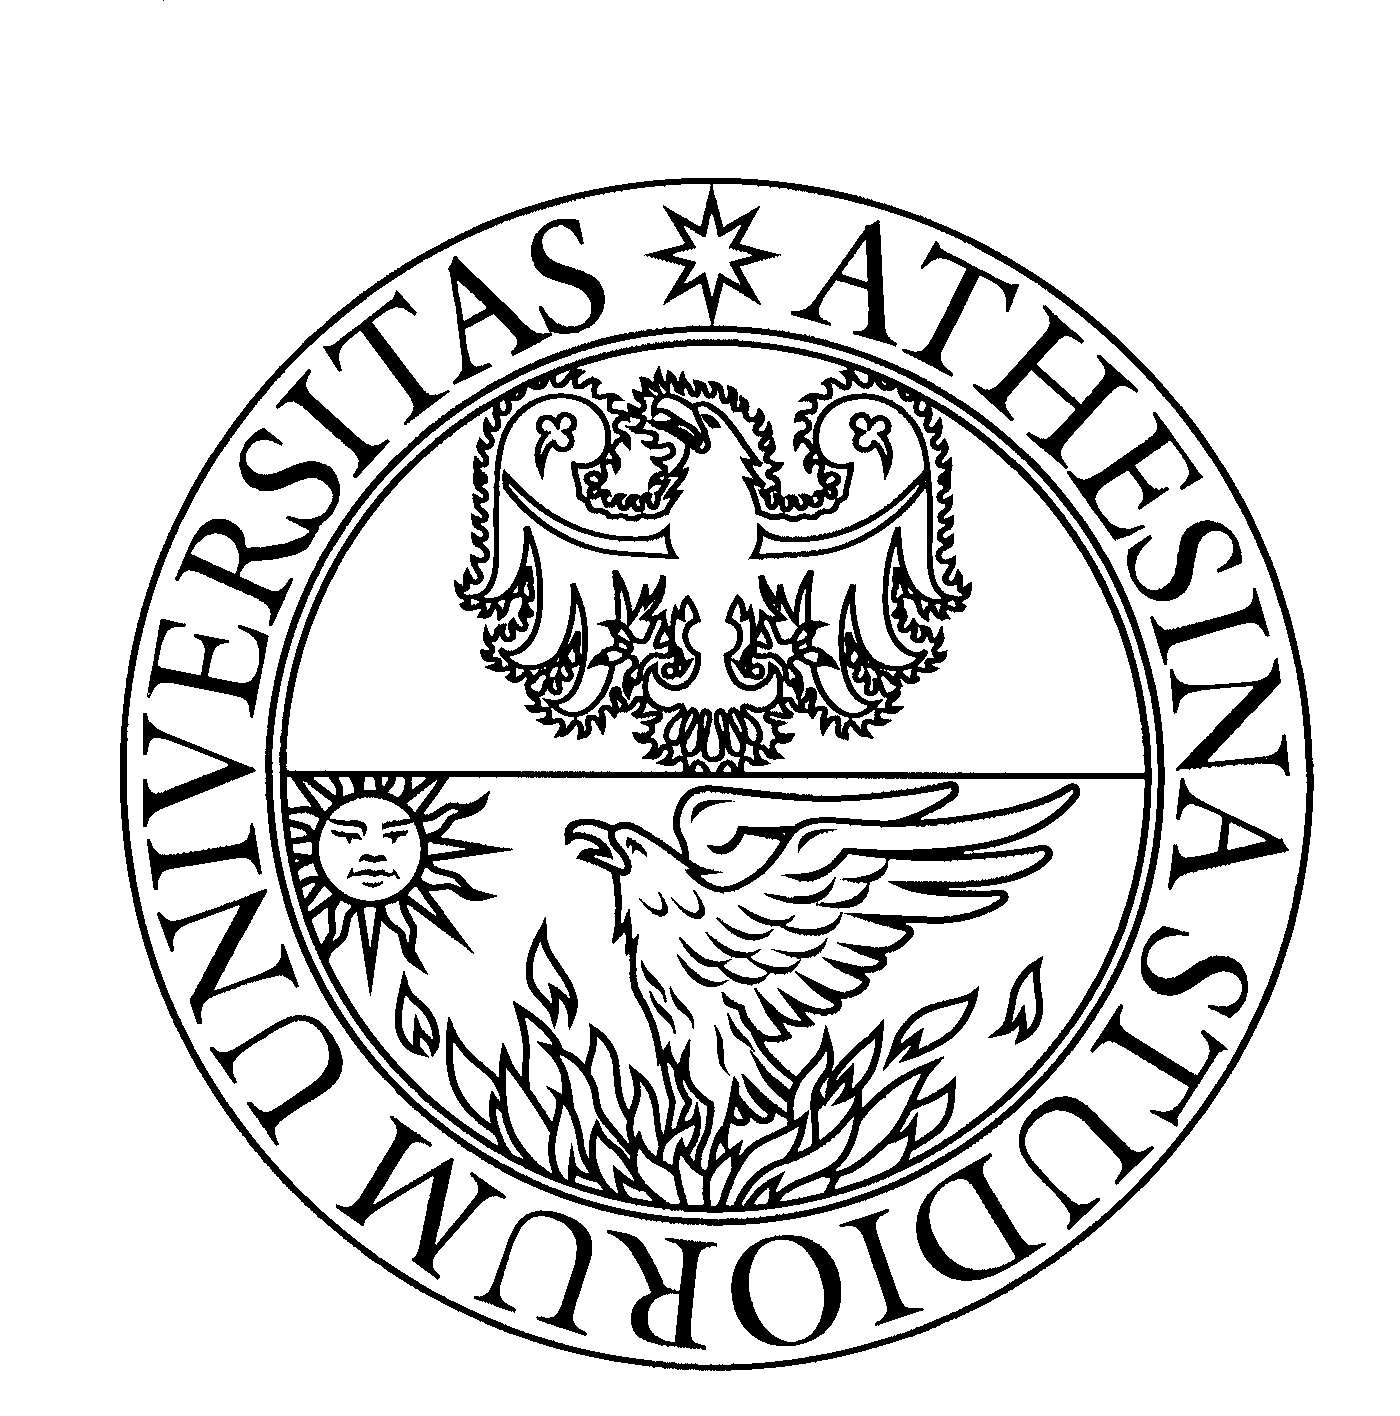
\includegraphics[width=0.3\linewidth]{logo_unitn.png}\\[1.25cm] % University/department logo - uncomment to place it
\textsc{\LARGE Master of Science in Economics}\\[2cm] % University programme
\textsc{\LARGE Master Thesis}\\[0.5cm] % Thesis type

\rule{\linewidth}{0.5mm}\\[0.75cm] % Horizontal line
{\Large \textbf{Using Machine Learning for Airbnb Price Prediction}}\\[0.5cm] % Thesis title
\rule{\linewidth}{0.5mm}\\[1cm] % Horizontal line

\begin{minipage}{0.4\textwidth}
\begin{flushleft} \large
Author:\\
\textsc{Duc Tuong Vu} % Author name - remove the \href bracket to remove the link
\end{flushleft}
\end{minipage}
\begin{minipage}{0.4\textwidth}
\begin{flushright} \large
Supervisor:\\
Prof. \textsc{Marco Bee} % Supervisor name - remove the \href bracket to remove the link
\end{flushright}
\end{minipage}\\[3cm]

\textsc{Academic Year 2020/2021}\\[0.25cm] % University requirement text

\vfill

\end{center}
\end{titlepage}

\clearpage
	\fancyhf{}
	\rhead{\thepage}
	\lhead{\textbf{Acknowledgments}}
\phantomsection
\addcontentsline{toc}{chapter}{Acknowledgments}
\pagenumbering{roman}
\chapter*{Acknowledgments}
\label{c:ack}
I would first like to pay special regards to my thesis advisor Professor. Marco
Bee of the Department of Economics and Management at the University of Trento.
The door to Professor Bee's office was always open whenever I ran into a
trouble spot or had a question about my research or writing. He consistently
allowed this paper to be my work but steered me in the right direction
whenever he thought I needed it.

Some special words of gratitude go to my friends who have always been a
significant source of support when things get a bit discouraging: Federico,
Nick, Ivan, Thai, Giang, Thuy, Hong. Thank you guys for always be there for me.

Nobody has more important to me in the pursuit of this project than the members
of my family. I would like to thank my parents for their great love and
understanding. To my brother Lieu, you are always in my heart, and  I hope you
get well soon. Most importantly, I wish to thank my brother Ly for providing me with
unfailing support and continuous encouragement throughout my years of study and
through the process of researching and writing this thesis.





\clearpage
	\fancyhf{}
	\rhead{\thepage}
	\lhead{\textbf{ \nouppercase{\leftmark}} }
\phantomsection
\addcontentsline{toc}{chapter}{Contents}
\tableofcontents

\clearpage
\phantomsection
\addcontentsline{toc}{chapter}{List of figures}
\listoffigures

\clearpage
\phantomsection
\addcontentsline{toc}{chapter}{List of tables}
\listoftables


\clearpage
	\fancyhf{}
	\rhead{\thepage}
	\lhead{\nouppercase{\leftmark}}
\pagenumbering{arabic}
\chapter{Introduction}
\label{c:intro}
\section{Motivation}
 \label{sec:motivation}

In recent years, the so-called sharing economy has spread all over the world.
People share access to resources such as their homes, cars, and even personal
time with other people in a peer-to-peer manner. One of the triumphant stories
of the sharing economy in the travel and hospitality industry is Airbnb. Airbnb
is a company that pioneers in deploying this business model to let individuals'
share' extra space in their homes with those who need temporary accommodation
via the online marketplace. In 2017, Airbnb generated approximately \$93 million
in profit out of \$2.6 billion in revenue \parencite{zaleski2018}.  As of 2020,
there are 2.9 million hosts on Airbnb, with over 7 million accommodations in
100,000 cities worldwide (Airbnb 2020).

An accurate prediction of the rental price helps maximize the Airbnb host's
profits and develop their business. So far, however, little attention has been
paid to empirical Airbnb rental price prediction. This indicates a need to have
an Airbnb rental price prediction model to address the research gap.

New York City (NYC) is one of Airbnb's most popular destinations with over
50,000 listings and ranked fourth in the most popular cities for booking
experiences \parencite{airbnbfacts}. With plenty of listing and booking
activities, New York City serves as an excellent example for the study of Airbnb
pricing.

\section{Objectives}
\label{sec:objectives}

This study systematically reviews the data for Airbnb in New York City, aiming:
\begin{enumerate}
  \item To employ machine learning techniques to build a model to predict Airbnb
    listing price in New York City.
  \item To identify which features of an Airbnb listing are most important  in
predicting the price
\end{enumerate}

\section{Research Methodologies}
This thesis contains four main research methodology:
\begin{enumerate}
\item Relative to collecting data method, we scrape the information about Airbnb
  listing from the InsideAirbnb website.
\item The data preprocessing step includes cleaning, data filtering,
  normalization, transformation, etc. The product of this step is the final
  training set ready for model fitting.
\item Exploratory analysis: we use visual methods to perform initial
  investigations on data to discover patterns and trends.
\item Model fitting:
  We applied several machine learning algorithms to make Airbnb rental price
  prediction.  The comparisons between the prediction performance of those
  models are presented in chapter \ref{c:data-analysis}.
\end{enumerate}

\section{Thesis Outline}
The overall structure of the study takes the form of four chapters. A short
description of the chapter is listed as follows:

\begin{itemize}

\item Chapter 2 begins by reviewing the past literature on the pricing in the
  sharing economy based accommodation rentals. Then, we will briefly introduce
  machine learning concepts and considerations when applying machine learning to
  predictive modeling. Furthermore,  we describe the machine learning algorithms
  used to solve the research question.

\item Chapter 3 - Data Analysis is concerned with the methodology used for this
study and the results we have obtained throughout our analysis.

\item Chapter 4 - Conclusions and Future Works: In this chapter, we will answer
  the research question based on the findings obtained in chapter
  \ref{c:data-analysis}.  Moreover, we will state some possible future
  adjustments to improve our results in this thesis.
\end{itemize}






\clearpage
\chapter{Background}
\label{c:background}

In this chapter, we start by presenting the concept of machine learning and
supervised regression learning. Then, we discuss the details of various
regression methods that have been explored during the course of this project.

\section{Machine Learning}

Machine learning refers to creating and using models that are learned from data.
Typically, our goal will be to use existing data to develop models that we can
use to predict various outcomes for new data. Examples of machine learning
applications can be found every where. Credit card companies use it to track
fraud.  The movie recommendation system is used by Netflix to suggest movies to
subscribers. Insurance companies use it to predict the risks of potential auto,
health, and life policyholder.

Most machine learning problems fall into one of two categories: supervised or
unsupervised. The details of machine learning outline are shown in
\ref{fig:ml-outline}.

\begin{figure}[H]\centering
    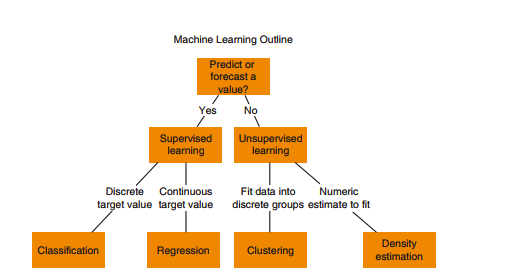
\includegraphics[width=\textwidth]{ml-outline.png}
    \caption{Machine Learning Outline}
    \label{fig:ml-outline}
    \source{\textcite{shah2020hands}}
\end{figure}

\subsection{Supervised Learning}

If our goal is to predict a specific outcome by learning how various predictors
and the response variables relate, we are dealing with \textbf{supervise
learning}. If the response variable is continuous, the problem becomes that of
\textit{regression}. If, on the other hand, the response variable is discrete,
this becomes a \textit{classification problem}. For instance, predicting the age
of a person, predicting house prices are regression problems, while predicting
the gender of a person, predicting whether a credit card transaction is
fraudulent are classification problems.

\subsection{Unsupervised Learning}
Unlike supervised learning, \textbf{Unsupervised learning} is a type of machine
learning that looks for hidden patterns in a data set with no output labels and
minimal human supervision. One of the most common unsupervised learning task is
clustering, where we group similar things together. For example, we can group
potential customers into different groups based on their characteristics, such
as income, age, gender, and shopping habits; we can group news articles into
different themes. if we are trying to explain the data by estimating underlying
processes that may be responsible for how the data is distributed, this becomes
a density estimation problem.

\section{Problem Formalization}

The problem of predicting the rental price can boil down to approximate a target
function \texttt{f} for the output variable rental price (Y) based on a set of
predictors such as \texttt{bathrooms}, \texttt{accomodates}...
We can describe the relationship between \texttt{price} (\texttt{Y}) and its
predictors $ X = (X_1, X_2, . . . , X_p) $ as followed:
\begin{eqnarray}
    Y = f(X) + \epsilon
    \label{eqn:relationship-eqn}
\end{eqnarray}

The  price of a listing can be predicted by:
\begin{eqnarray}
    \hat{Y} = \hat{f}(X)
    \label{eqn:predicted-value}
\end{eqnarray}

\section{Quantitative Measures of Performance}

Selecting the best method among many different statistical learning approaches
can be one of the practitioners' most daunting tasks.  One particular approach
may work best on a particular data set, but some other methods may perform
better on a similar but different data set.  Therefore, it is critical to select
which method produces the best results for any given data set.  To assess a
particular model's predictive performance on a given data set, we need some way
to measure how well its predictions match the observed data.
In this study, we use two standard criteria: mean squared error and coefficient
of determination.

\subsection{Mean Squared Error}
When an outcome is a number (regression problem), the most commonly used method
for characterizing a model's predictive capabilities is to use the mean squared
error (MSE), which is:

\begin{eqnarray}
    \label{eqn:mse}
    MSE = \frac{1}{n} \sum_{i=1}^{n}(y_i - \hat{f}(x_i))^2
\end{eqnarray}
where $\hat{f}(x_i)$ is the prediction that $\hat{f}$ gives for the $i^{th}$
observation. If the predicted responses are very close to the actual responses,
the MSE will be small and vice versa.

In general, we do not care how well the method works  on the training
data. Instead, we are interested in the accuracy of the test MSE predictions we
obtain when applying our method to previously unseen test data. Therefore, we
want to choose the approach that gives the lowest test MSE instead of the lowest
training MSE.

\subsection{Coefficient of Determination}
We also use the coefficient of determination ($R^2$) to measure the proportion
of the information in the data explained by the model.  For example, an $R^2$
value of 0.8 means that the model can explain  80 percent of the outcome's
variation. An $R^2$ of 1 indicates that the regression predictions perfectly fit
the data. It should be noted that $R^2$ is a measure of correlation, not
accuracy.
$R^2$ is calculated as the correlation coefficient between the
observed and predicted values and squares it:
\[ R^2 = 1 - \frac{SS_{res}}{SS_{tot}}\]
where $SS_{res}$ is the sum of squares of residuals and $SS_{tot}$ is the total
sum of squares (proportion to the variance of the data)

\section{Variance-Bias Tradeoff}

From \cite{james2013introduction}, the expected test MSE, for a given value $x_0$, can be broken down into three
parts as followed:
\begin{eqnarray}
E(y_0 - \hat{f}(x_{0}))^2 =  \textrm{Var}(\epsilon) +
[\textrm{Bias}(\hat{f}(x_{0})]^2 + \textrm{Var}(\hat{f}(x_{0}))
\label{eqn:variance-bias-tradeoff}
\end{eqnarray}

%irreducible term
The first term is the irreducible error, which cannot be reduced regardless of
what algorithm we use. It is a measure of the amount of noise in our data. No
matter how good we make our model, our data will have a certain amount of noise
or irreducible errors that can not be removed.

%bias term
The second term is the model's squared bias, reflecting how close the target
function (\texttt{f}) can get to the real relationship between the predictors
and the outcome.  A model with high bias pays very little attention to the
training data and oversimplifies the model. It always leads to increased errors
in training and test data.  An example of a high bias model is linear
algorithms. While having a high bias makes them fast to learn and more
interpretable, they are generally less flexible.  As a result, they usually have
a poor predictive performance on complex problems that fail to satisfy the
simplifying assumptions of the linear regression algorithm.

%Variance term

Variance is how much the value of target function (\texttt{f}) will vary if we
use different training data. In contrast to high bias algorithms, models with
high variance focus too much on the training data and do not generalize the data
it has not seen before. Consequently, such models may perform very well on
training data but have high test prediction errors.  It is generally true that
more complex models can have very high variance, which leads to
\textit{overfitting}, which essentially means they follow the errors or noise
too closely.  Choosing an overly simple model might lead to
\textit{underfitting}, which means it will not learn the data's underlying
structure, so its prediction is bound to be inaccurate, even on the training
data.

As can be seen in equation \ref{eqn:variance-bias-tradeoff}, minimizing the test
MSE means reducing the combination of bias and variance. Ideally, we want to
have a model that has low bias and low variance. Unfortunately, it is typically
impossible to do both simultaneously. If our model is too simple and has very
few parameters, it may have high bias and low variance. On the other hand, if
our model is too complicated, we start focusing too much on each data point in
our training set, it will have high variance and low bias.

There is no escaping the relationship between bias and variance in machine
learning. Therefore, this study's strategy is to try various machine learning algorithms
with different variance-bias tradeoff levels to decide which is the best
model to achieve a low bias and low variance model. In other words, we seek to
find a sweet spot in between the variance bias spectrum that will yield the best
generalization performance. These algorithms will be described in the next
section.

\section{Models and Algorithms}

\subsection{Linear Regression}
\label{linear-regression}

Linear regression is the simplest and earliest predictive method.
Multiple regression analysis is the foundation of Hedonic price
modelling which has been widely used in real estate, tourism, and hotels to
explore the relationship between a product's price and its characteristics
\parencite{rosen1974hedonic}.

Hedonic pricing theory states that a product's price can be regarded as a
function of the product's measurable, utility-affecting attributes or
characteristics.  Accordingly, We can decompose Airbnb accommodation into
features that impact the overall product's quality and provide consumers with
value and satisfaction.  These may include the number of bedrooms, the number of
capacities, number of reviews it receives, and amenities.
We can specify the hedonic price function of Airbnb listings as follows:
\begin{eqnarray}
    Y = \beta_0 + \beta_1 X_1 + \beta_2 X_2 + ... + \beta_p X_p + \epsilon
\end{eqnarray}

where $X_j$ represents the $j^{th}$ predictor and $\beta_j$ quantifies the
association between that variable and the response

Given estimates $\hat{\beta_0}$,$\hat{\beta_1}$,...,$\hat{\beta_p}$ , we can
make predictions using the formula:
\begin{eqnarray}
  \hat{y} = \hat{\beta_0} + \hat{\beta_1} X_1 + \hat{\beta_2} X_2 + ... + \hat{\beta_p} X_p
\end{eqnarray}

The parameters are estimated using the least-squares approach in multiple linear
regression. We choose $\beta_0$, $\beta_1$, . . . , $\beta_p$ to minimize the
sum of squared residuals.
\begin{equation}
\begin{split}
\textrm{RSS} & = \sum_{i=1}^{n}(y-\hat{y_i})^2 \\
   & =\sum_{i=1}^{n}(y_i - \hat{\beta_0} - \hat{\beta_1} x_{i1} - \hat{\beta_2} x_{i2} - ... - \hat{\beta_p} x_{ip})^2
\end{split}
\end{equation}

Given some minimal premises about the distribution of the residuals \footnote{
the error terms are independent, uncorrelated and normally distributed with a
mean of zero and constant variance  (a.k.a. homoskedasticity)}, the hedonic
regression parameter estimates that
minimize SSE are the ones that have the least bias of all possible parameter
estimates (\textcite{graybill1976theory} ). Therefore, these estimates minimize
the bias element of the bias-variance trade-off.

While having a distinct advantage of highly interpretable, the hedonic
regression model suffers from overfitting \parencite{harrell2015regression}.
In a situation in which  there is little or no theory available to guide on
selecting the predictors, we want to include in our model as many features as
possible.  However, we run the risk of including irrelevant features that
actually have no relation to the dependent variable being predicted, thus might
not improve the predictive power on future data.

\subsection{Penalized Regression Models}
\label{ssec:penalized_regression_models}

Overfitting frequently occurs in the regression setting
\parencite{harrell2015regression}.  While a model with many explanatory
variables that have no relation to the response might increase the model's
performance on the training data, it might not generalize well on the validation dataset.

To lessen the effect of overfitting, we use regularization techniques, which
essentially constrain or regularize the coefficient estimate towards zero.
Consider the case of the linear model with two parameters $\theta_0$ and
$\theta_1$. This gives the learning algorithm two degrees of freedom to
accommodate the model to the training data. If we forced $\theta_1$ = 0, the
algorithm would have only one degree of freedom and would find it more difficult
to fit the data properly. If we allow the algorithm to shrink the $\theta_1$  to
a small amount, the learning algorithm degrees of freedom will be between one
and two. It will produce a simpler model than one with two degrees of freedom,
but more complex than one with just one.  Either way, we can achieve a simpler
model that can generalize well to unseen data. Therefore, applying regularization can significantly reduce the model's variance.
In this section, we present the two best-known methods for regularization, ridge
regression, and the lasso.

\subsubsection*{Ridge Regression}

Ridge Regression (\textcite{hoerl1970ridge})  regularizes the parameter
estimates by adding a penalty to the MSE. The algorithm is very similar to least
squares, except that the coefficients ridge are estimated by minimizing a
slightly different quantity. In particular, the ridge regression coefficient
estimates  are the values that minimize:
\begin{eqnarray}
    \label{eqn:ridge-optimal}
    \sum_{i=1}^{n}(y_i -\beta_0 - \sum_{j=1}^{p}\beta_j x_{ij}) ^ 2 + \lambda
    \sum_{j=1}^{p}\beta_{j}^2 = RSS + \lambda \sum_{j=1}^{p}\beta_{j}^2
\end{eqnarray}
In  Equation  ~\ref{eqn:ridge-optimal} we made a trade-off between two different
criteria. As with least squares, ridge regression seeks coefficient estimates
that fit the data well, by making the RSS small. But, the second term, $\lambda
\sum_{j=1}^{p}\beta_{j}^2$ signifies that a second-order penalty (i.e., the
square) is being used on the parameter estimates.
This shrinkage penalty is small when $\beta_1$,...,$\beta_p$ are close to zero,
and so it has the effect of shrinking penalty the estimates of $\beta_j$ towards
zero.

When $\lambda = 0$, the penalty term has no effect, and ridge regression is the same
as least squares estimates. However, as $\lambda \to \infty$, the influence of
the shrinkage penalty increases, and the ridge regression will shrink the
estimates towards  zero.
In contrast to least squares, which produces only one set of coefficient
estimates, ridge regression will generate a different set of coefficient
estimates, $\hat{\beta}_{\lambda} ^ {R}$, for each value of $\lambda$.

\subsubsection*{Lasso Regression}

One drawback of ridge regression that it does not set any of the parameter
estimates equal to 0. Therefore, the model does not conduct feature selection.
Least Absolute Shrinkage and Selection Operator (Lasso)
\parencite{tibshirani1996regression} model is a modern
alternative to ridge regression that overcomes this disadvantage. The name comes
from its functionality that it does not only shrink coefficients towards zero,
but it also performs feature selection.


The lasso  coefficients, $\hat{\beta}^L$ , minimize the quantity:
\begin{eqnarray}
    \label{eqn:lasso-optimal}
    \sum_{i=1}^{n}(y_i -\beta_0 - \sum_{j=1}^{p}\beta_j x_{ij}) ^ 2 + \lambda
    \sum_{j=1}^{p} \mid \beta_{j} \mid= RSS + \lambda \sum_{j=1}^{p} \mid \beta_{j} \mid
\end{eqnarray}
Notice that the lasso and ridge regression have similar formulations. The only distinction is in the penalty term. In particular, the $\beta_j^2$ term in the ridge regression penalty (6.5) has been replaced by $\mid \beta_{j} \mid$ in the lasso penalty
The implication of this modification is that penalizing the absolute values has the effect of setting some of the coefficient estimates to be exactly equal to zero for some value of $\lambda$. Thus the lasso yields models that simultaneously use regularization to improve the model and to conduct feature selection.

We can formulate the lasso and ridge regression coefficient estimates in
\ref{eqn:lasso-optimal} and \ref{eqn:ridge-optimal} as solving following
problems:

\begin{equation}
    \label{eqn:ridge-optimal}
    \begin{aligned}
    \min_{\beta} \quad \sum_{i=1}^{n}(y_i -\beta_0 - \sum_{j=1}^{p}\beta_j
    x_{ij}) ^ 2  \quad \textrm{subject to} \quad \sum_{j=1}^{p}\mid\beta_j\mid
    \leq s
    \end{aligned}
\end{equation}
and
\begin{equation}
    \label{eqn:lass-optimal}
    \begin{aligned}
    \min_{\beta} \quad \sum_{i=1}^{n}(y_i -\beta_0 - \sum_{j=1}^{p}\beta_j
    x_{ij}) ^ 2  \quad \textrm{subject to} \quad \sum_{j=1}^{p}\beta_j^2\leq s
    \end{aligned}
\end{equation}

In the figure \ref{fig:feature-selection}, we illustrate why the lasso performs
feature selection, while ridge regression does not.To simplify the problem, we
consider only two parameters $\beta_1$ and $\beta_2$.
The elliptic centered around $\hat{\beta}$ are contours of the sum of squares
error with the OLS estimator in the center. All of the points on a given ellipse
has the same value of RSS. The diamond and circle represent the lasso and ridge
regression constraints in \ref{eqn:lasso-optimal} and \ref{eqn:ridge-optimal}.

The lasso and ridge regression coefficient estimates are the first point at
which an ellipse touches the constraint set.
Note that the ridge regression has a circular constraint with no sharp points.
This intersection will not generally occur on an axis. So the ridge regression
coefficient estimates will be exclusively non-zero. However, the lasso
constraint has corners at each of the axes, and so the ellipse will often
intersect the constraint region at an axis. When this occurs, one of the
coefficients will equal zero.In this way, the lasso performs \textit{feature
selection}.
\begin{figure}[H]\centering
    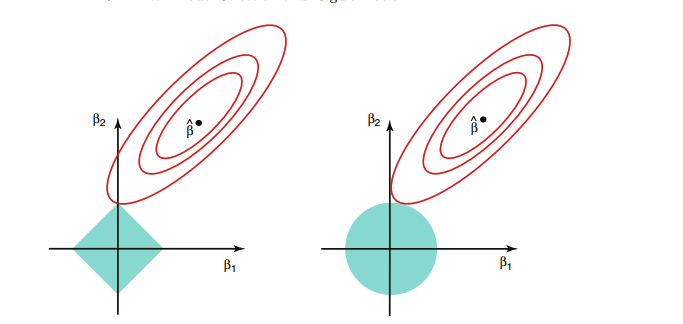
\includegraphics[width=\textwidth]{feature-selection1.png}
    \caption{Illustration of two dimensional case of estimation for the lasso
    (left) and the ridge regression (right)}
    \label{fig:feature-selection}
    \source{\textcite{james2013introduction}}
\end{figure}

\subsubsection*{Selecting the Tuning Parameter}

Choosing an optimized value of tuning parameter $\lambda$ is critical when
implementing the ridge and the lasso regression.
We do not want to choose $\lambda$ too small due to the low restriction. On the
other hand, when $\lambda$ is very large, the restriction is more substantial
than it is desired. We handle the problem of the optimal value of  by using a
cross-validation technique. \textcite{efron1994introduction} introduce the algorithm, which describes
the procedure of cross-validation.

\begin{algorithm}[H]
\setstretch{1.35}
\SetAlgoLined
\renewcommand{\labelenumi}{(\Roman{enumi})}
Split the data into K roughly equal-sized parts.

For the $k^{th}$ part, fit the model to the other K − 1 parts of the data, and
calculate the mean squared error of the fitted model when predicting the
$k^{th}$ part of the data.

Repeat step 2 for k = 1, 2, . . . , K and average the K estimates of mean
squared error $MSE_1$, $MSE_2$,..., $MSE_k$.

For each tuning parameter value $\lambda$, compute the average error over all
folds \[CV_{(k)} = \frac{1}{k} \sum_{i=1}^{k} MSE_i\]

 \caption{K-Fold Cross Validation}
\end{algorithm}


We choose a grid of $\lambda$ values and calculate the cross-validation error
for each value of $\lambda$. We then select the tuning parameter value for which
the cross-validation error is smallest.

\subsection{Boosting}

All the approaches reviewed so far suffer from the fact that they use a single
model for predicting the response variable. Hence the ability to choose a
suitable model is crucial to have any chance to obtain good results.
Machine Learning practitioners have to consider many factors such as
the quantity of data, the dimensionality of the space, and distribution
hypothesis to find a high predictive power model.

Boosting, on the other hand, is an an ensemble technique in which several weak
models such as decision trees  are combined to achieve a stronger one.The
general idea of most boosting methods is to train predictors sequentially, each
trying to correct its prede‐ cessor.

\subsubsection*{Regression Trees}

Regression Tree is a type of decision trees  used to predict continuous
numeric values (e.g. the price of a house, or a patient's length of stay in a
hospital). In a regression tree, each leaf represenet a numeric value.

A regression tree is recursively constructed through a binary partitioning
process. We first select the predictor  and the cut point s such that splitting
the predictor space into the two regions (S1 = {${X|X_j <s}$} and S2 = {${X|X_j
> s}$}) such that the overall sums of squares error are minimized:

\begin{eqnarray}
  \textrm{SSE} = \sum_{i\in S_1}^{n}(y-\bar{y_1})^2 + \sum_{i \in S_2}^{n}(y-\bar{y_2})^2
\end{eqnarray}


where $\hat{y_1}$ and  $\hat{y_1}$ are the mean response for  training set within groups
S1 and S2, respectively.

We repeat the process, looking for the best predictor and best cutpoint to split
the data further to minimize the sums of squares errors within each group. The
recursive partitioning of the data continues until a stopping criterion reached
for instance, we may continue until no region contains more than 20
observations.
We predict the response for a given test data point using the average value of
the training observations in the group to which that test observation belongs.



\subsubsection*{Gradient Boosting}

While having an advantage of being easily be visualized and understood, the main
downside of decision trees is that they tend to overfit and provide poor
generalization performance. Therefore, in most applications, the ensemble
methods such as boosting are usually used in place of a single decision tree.

The underlying idea behind ensemble learning is that by aggregating the
predictions of a group of predictors (such as classifier or regressors) we will
ofter get better predictons than the best individual predictor (\textit{wisdom of the
crowd}).
According to ensemble learning theory, weak learners are models that perform not
so well by themselves either because they have a high bias or because they have
too much variance. Then the idea of ensemble methods is to reduce bias and/or
variance of such weak learners by combining several of them together to create a
strong leader that achieves better predictive performance.

Boosting refers to any ensemble method for primarily reducing bias, and also
variance by combining several weak learners into  a strong learner.  Being
mainly focused at reducing bias, the base learners that are often considered for
boosting are models with low variance but high bias such as shallow decision
trees with only a few depths.
Another reason for using shallow trees in boosting is that it makes the model
smaller in terms of memory and makes prediction faster.

%While having an advantage of being easily be visualized and understood, the main
%downside of decision trees is that they tend to overfit and provide poor
%generalization performance.  Therefore, in most applications, the ensemble
%methods such as boosting are usually used in place of a single decision tree.
%Trees can make excellent base learners for boosting for the following reasons:
%\begin{enumerate}
    %\item By limiting their depth, they can be weak learners.
    %\item We can add together separate trees easily.
    %\item Trees can be created quickly.
%\end{enumerate}

While there are many boosting methods available, in this study, we focus on
Gradient boosting trees and its high-performance implementation, XGBoost. In
gradient boosting trees,  regression trees are chosen  as the base learners.
%We illustrate this approach in Figure ~\ref{fig:gradient-boosting-illustration}

%\begin{figure}[H]\centering
    %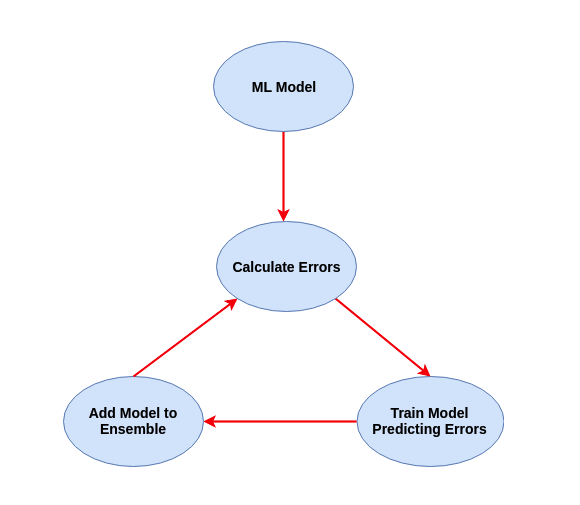
\includegraphics[width=0.75\textwidth]{gradient-boosting-illustration.png}
    %\caption{Gradient Boosting Approach}
    %\label{fig:gradient-boosting-illustration}
%\end{figure}

\textcite{kuhn2013applied} illustrate the Gradient Boosting for
Regression algorithm as followed:

\begin{algorithm}[H]
\setstretch{1.35}
\SetAlgoLined

\renewcommand{\labelenumi}{(\Roman{enumi})}
Select tree depth, D, and number of iterations, K

Compute the average response, $\bar{y}$, and use this as initial predicted value
for each observation in the training set.

\For{$k\gets0$ \KwTo $K$ }{
    Compute the residual, the difference between observed value and the
    \textit{current} predicted value, for each observation.

    Fit a regression tree of depth, D, using the residuals as the response.

    Predict each observation using regression fit in the previous step.

    Update the predicted value of each observation by adding the previous
    iteration's predicted value to the predicted value generated in the previous
    step.

    }
 \caption{Simple Gradient Boosting for Regression}
\end{algorithm}

We can find the the optimal value of tree depth (D) and the number of
iterations (K) by using cross-validation techniques.

\subsubsection*{XGBoost}

%XGBoost is an end-to-end tree boosting system developed by
%\textcite{chen2016xgboost} based on a
%gradient boosting framework. Since its introduction in 2014, this algorithm has
%been credited with winning numerous Kaggle competitions and driving under the
%hood for several cutting-edge industry applications. Furthermore, XGBoost has
%been shown to provide state-of-the-art results for diverse problems, including
%web text classification, customer behavior prediction, motion detection, and
%malware classification \textcite{chen2016xgboost}.
XGBoost is an end-to-end tree boosting system developed by
\textcite{chen2016xgboost} based on a
gradient boosting framework.  XGBoost has been shown to provide state-of-the-art
results for diverse problems, including web text classification, customer
behavior prediction, motion detection, and malware classification
\parencite{chen2016xgboost}.

\textcite{nielsen2016tree} shows some features of XGBoost that make it stand out
of from the rest of other gradient boosting algorithms. That is:
\begin{itemize}
    \item Clever penalization of trees
    \item A proportional shrinking of leaf nodes
    \item Newton Boosting
    \item Extra randomization parameter
    \item Implementation on single, distributed systems and out-of-core computation
\end{itemize}
%Several reasons explain why XGBoost is popular in the machine learning
%community, which includes:
Besides these superior features, there are other reasons why XGBoost is getting
popular in the machine learning community:
\begin{itemize}
    \item Can solve a wide range of applications such as regression,
        classification, ranking, and user-defined prediction problems.
    \item Portability: Runs smoothly on Windows, Linux, and OS X.
    \item Languages: Supports all major programming languages, including C++,
        Python, R, Java, Scala, and Julia.
    \item Cloud Integration: Supports AWS, Azure, and Yarn clusters and works
        well with Flink, Spark, and other ecosystems.
\end{itemize}

%Since its introduction in 2014, this algorithm has
%been credited with winning numerous Kaggle competitions and being the driving
%force under the hood for several cutting-edge industry applications. Futhermore,
%XGBoost has been shown to provide state-of-the-art results for diverse problems,
%including web text classification, customer behavior prediction, motion
%detection, and malware classification \textcite{chen2016xgboost}
%\textcite{nielsen2016tree}.

While XGBoost is suitable for predicting, it does so at the expense of its
interpretability.  As shown in Figure
\ref{fig:flexibility-interpretability-tradeoff}, compared to restrictive models
such as Lasso or Least Squares, Boosting is a highly flexible (complex) approach
that is harder to interpret.

\begin{figure}[H]\centering
    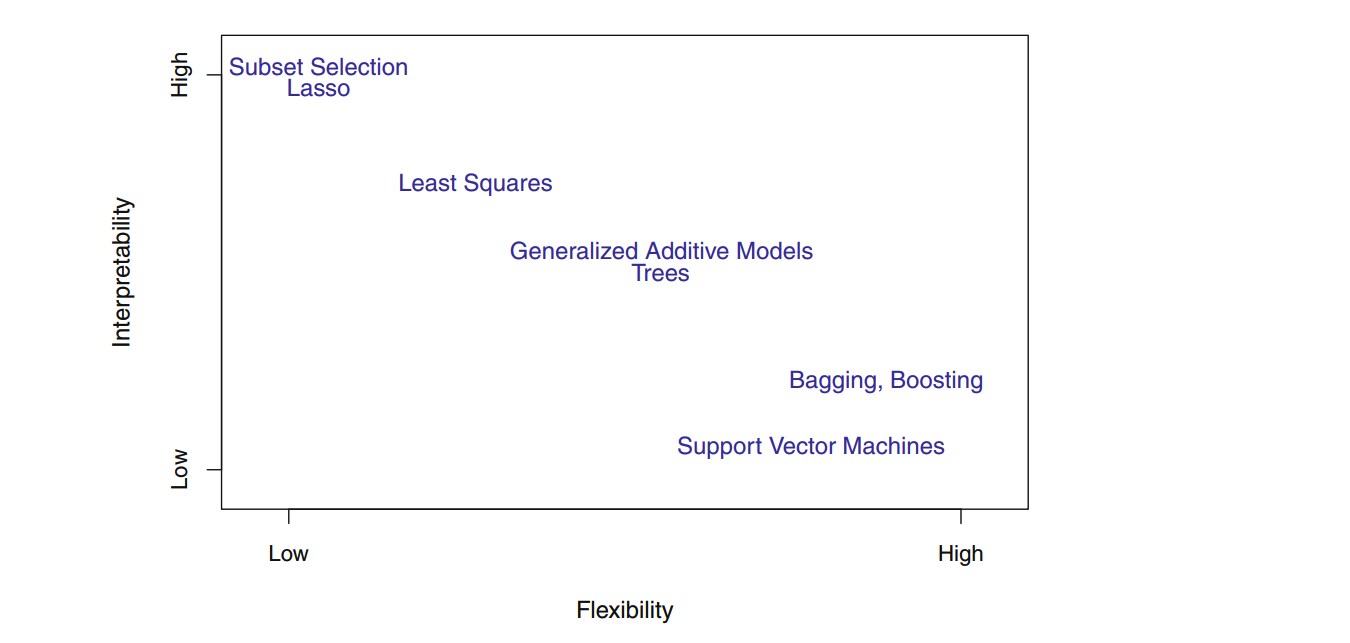
\includegraphics[width=\textwidth]{flexibility-interpretability-tradeoff.png}
    \caption{Interpretability and Flexibility Tradeoff}
    \label{fig:flexibility-interpretability-tradeoff}
    \source{\textcite{james2013introduction}}
\end{figure}




\clearpage
\chapter{Data Analysis}
\label{c:data-analysis}
\section{Data Acquisition}
\label{sec:data_acquisition}

The dataset used for this study comes from the Inside Airbnb website
\textcite{Airbnb}. This independent initiative collects Airbnb data for more than 30
major cities around the world that scrapes Airbnb listings, reviews, and
calendar data from multiple cities worldwide. The dataset  was scraped on
December 4, 2019, contains information about the location (latitude and
longitude coordinates) of all Airbnb listings in New York City and data about
the hostname and ID, room type, price, minimum nights, number of reviews
listings per host, and availability...

The raw data is quite untidy and has some weaknesses. The major one is that it
only includes the advertised price (sometimes called the ‘sticker’ price). The
sticker price is the overall nightly price advertised to potential renters,
rather than the actual average amount paid per night by previous guests. A host
can set the advertised prices to any arbitrary amount, and those that do not
have much experience with Airbnb will often set these to unreasonable prices,
such as too low (e.g., \$0) or very high (e.g., \$10,000) amounts.

These variables are listed and defined in Table ~\ref{tab:variable-list}.

\section{Data Preprocessing }
\label{sec:data_cleaning}

Real-world data is often dirty; that is, it is in need of being cleaned up
before it can be used for the desired purpose such as visualization, model
building. This is often called data pre-processing.
Since there are several reasons why data could be “dirty,” there are just as
various techniques to “clean” it.  For this analysis, we will take a look at
three key methods that illustrate ways in which data may be “cleaned,” or better
organized, or scrubbed of potentially incorrect, incomplete, or duplicated data.

\subsection{Data Filtering}

Following \textcite{wang2017price}, this study filtered the listings with at
least one online customer review to guarantee that our sample listings were
"active." This view is supported by \textcite{ye2009impact}  which confirms that online
review ratings are associated with hotel-room sales, indicating that reviews
suggest real transactions.

\subsection{Removing Predictors}

There are three reasons why we should consider removing predictors before
modeling. First, fitting a model with fewer predictors reduces computational
time and complexity. Second, removing highly correlated features makes the model
more parsimonious and interpretable model.  Lastly, some models can be crippled
by predictors with degenerate distributions.  Therefore, eliminating the
problematic predictors prior to fitting a model can significantly improve model
performance and stability.
\begin{itemize}

    \item We remove  predictors with a single unique value as they are  zero
        variance predictors. These predictors are \texttt{has\_availability},
        \texttt{host\_has\_profile\_pic},\texttt{requires\_license},
        \texttt{is\_business\_travel\_ready},
        \texttt{require\_guest\_phone\_verification},\newline
        \texttt{require\_guest\_profile\_picture} (See
        \ref{fig:histogram-feature-distribution}) .
    \item It is beyond the scope of this study to explore the natural language
        processing for predictive modeling.  Therefore,  we will drop free-text
        columns for now, as will other columns that are not useful for
        predicting price (e.g., \texttt{url}, \texttt{hostname}, and other host-related features
        unrelated to the property).

    \item We drop feature which  adds relatively little information, or are
        relative unhelpful in differentiating between different listings.

\end{itemize}

\subsection{Dealing with Missing Values}

Missing data is a common issue in many data analysis applications.  Data may be
missing due to problems with the process of collecting data or equipment
malfunction. Some data may get lost due to system or human error while storing
or transferring the data.

There are two approaches we take to handle missing
data:
\begin{enumerate}
    \item Filling out missing value :  we drop the predictors
        that contain a majority of null entries as in Table
        ~\ref{tab:missing-value}.
    \item Filling in missing value:we perform data imputation, which means
        filling the missing data with some estimated ones. In particular,

        \begin{itemize}

            \item Missing values in numeric features such as the number of
                bathrooms (\texttt{bathrooms}) bathrooms, the number of bedrooms
                (\texttt{bedrooms}), the number of beds (\texttt{beds}) will be
                replaced with the median.

            \item For monetary features such as the amount required as a
                security deposit (\texttt{security\_deposit}), the amount of the cleaning
                fee (\texttt{cleaning\_fee}), the price per additional guest
                (extra\_people), having a missing value for them is the same as
                having the value of \$0, so the missing values will be replaced
                with 0. Similarly, an amenity that has a missing value will be replaced with 0.

        \end{itemize}
\end{enumerate}

\begin{table}[htp]
    \centering
    \caption{Columns with majority of null values}
    \label{tab:missing-value}
{\small
\begin{tabular}{lrr}
\toprule
{} &  count &  percentage \\
\midrule
host\_acceptance\_rate &  50599 &      100.00 \\
jurisdiction\_names   &  50583 &       99.97 \\
license              &  50577 &       99.96 \\
square\_feet          &  50213 &       99.24 \\
monthly\_price        &  45683 &       90.28 \\
weekly\_price         &  44945 &       88.83 \\
\bottomrule
\end{tabular}
}
\end{table}

\subsection{Feature Construction}

\begin{itemize}

    \item We convert DateTime columns such as the date that the host first joined Airbnb
        (\texttt{host\_since}) to measure the number of days a host has been on
        the platform, measured from the date that the data was collected
        (\texttt{host\_days\_active}).

    \item We create a new feature that measures the number of days between the first
        review and  the date we collect the data
        (\texttt{time\_since\_first\_review}) from
        the feature the date of the first review (\texttt{first\_review}).

    \item We can compute the number of days between the most recent review and
        the date the data was scraped (\texttt{time\_since\_last\_review}) using the date of the
        most recent review (\texttt{last\_review}).
\end{itemize}

\subsection{Binning Predictors}

We want to discretize continuous data into "bins" for analysis in many situations, especially when that data has a wide range.
Binning, also known as quantization, is a useful technique for converting continuous numeric features into discrete ones (categories).
In our dataset, we peform the following binning:
\begin{itemize}

    \item The feature that measures proportion of messages that the host replies
(host\_response\_rate) will be bin into four categories '0-49\%', '50-89\%',
'90-99\%', '100\%',

    \item The number of days between the first review and the date we collect the data
        (\texttt{time\_since\_first\_review}) will be bin into '0-6 months', '6-12 months', '1-2
    years', '2-3 years', '4+ years'

    \item The number of days between the most recent review and the date the data was
        scraped (\texttt{time\_since\_last\_review}) will be bin into '0-2 weeks','2-8 weeks',
    '2-6 months', '6-12 months', '1+ year'

    \item Review scores rating (\texttt{review\_scores\_rating}) will be bin into following
        categories '0-79/100', '80-94/100', '95-100/100'
\end{itemize}



\subsection{Data Transformation}

\subsubsection*{Feature Scaling}

Feature scaling is an essential step in the preprocessing process, as some
machine learning algorithms do not perform well when the numerical input
attributes have very different scales.

Feature scaling through standardization (or Z-score normalization) is straightforward and
common-used in the machine learning community.
Standardization means that we rescale the predictors so that they have a zero
mean and standard deviation 1.  We first compute the mean and standard deviation
for the feature and scale it based on:
\[x^{'} = \frac{x - \bar{x}}{\sigma}\]
where $x$ is the original feature vector, $\bar{x} = \textrm{average(x)}$ is the mean of
that feature vector, and $\sigma$ is its standard deviation.

\noindent In our dataset we use  a transformer called StandardScaler from Scikit-Learn for
standardization.

\subsubsection*{Transformation to Resolve Skewness}

Many models assume a normal distribution, which means data are symmetric about
the mean.
Unfortunately, our real-life datasets do not always follow the normal
distribution.  Instead, they are usually skewed, which makes the results of our
statistical analyses invalid.

Figure \ref{fig:histogram-before-transform}
shows the distribution of numerical features. We notice
that most of the predictors have a heavy-tailed distribution. Therefore we
transform them by replacing them with their logarithm. Figure
\ref{fig:histogram-after-transform} shows the result;
some of the distributions become normal. More importantly, the outcome variable
price appears much more normally distributed.

\subsection{Handling Categorical Attributes}

One of the significant problems with machine learning is that many algorithms
cannot work directly with categorical data (non-numerical values).  Hence, we
need a way to convert categorical data into a numerical form, and our machine
learning algorithm can take in that as input. In this study, we use  One-Hot
Encoding, one of the most widely used encoding techniques.  One-hot encoding is
processed in 2 steps:
\begin{enumerate}
    \item First, we split categories into different columns.
    \item We then put 0 for others and 1 as an indicator for the appropriate column.
\end{enumerate}

There is a very simple way to encode the data in python pandas library, using
the \texttt{get\_dummies()} function.

\section{Exploratory Data Analysis}

Before embarking on developing statistical models and generating predictions, it
is essential to understand your data. This is typically done using conventional
numerical and graphical methods. \textcite{tukey1977exploratory} advocated the practice
of exploratory data analysis (EDA) as a critical part of the scientific process.

We present the descriptive statistics of variables in Table
\ref{tab:descriptive-statistic}

\subsection{Numerical Features}
\label{sec:numerical_features}

\subsubsection*{Price}

The nightly advertised prices range from \$0 to \$10,000. The range is so broad
because hosts do not understand how to set Airbnb advertised prices.  Figure
~\ref{fig:price-distribution-1000} and Figure ~\ref{fig:price-distribution-200}
 show the distributions of price up to \$1,000 and \$200 respectively. While the
price's range is extensive, most of its values concentrate on the range \$10 to
\$1000.  Hence, for minimal values under \$10, we will increase them to \$10,
and values above \$1,000 will be reduced to \$1,000.

\begin{figure}[!htbp] \centering
    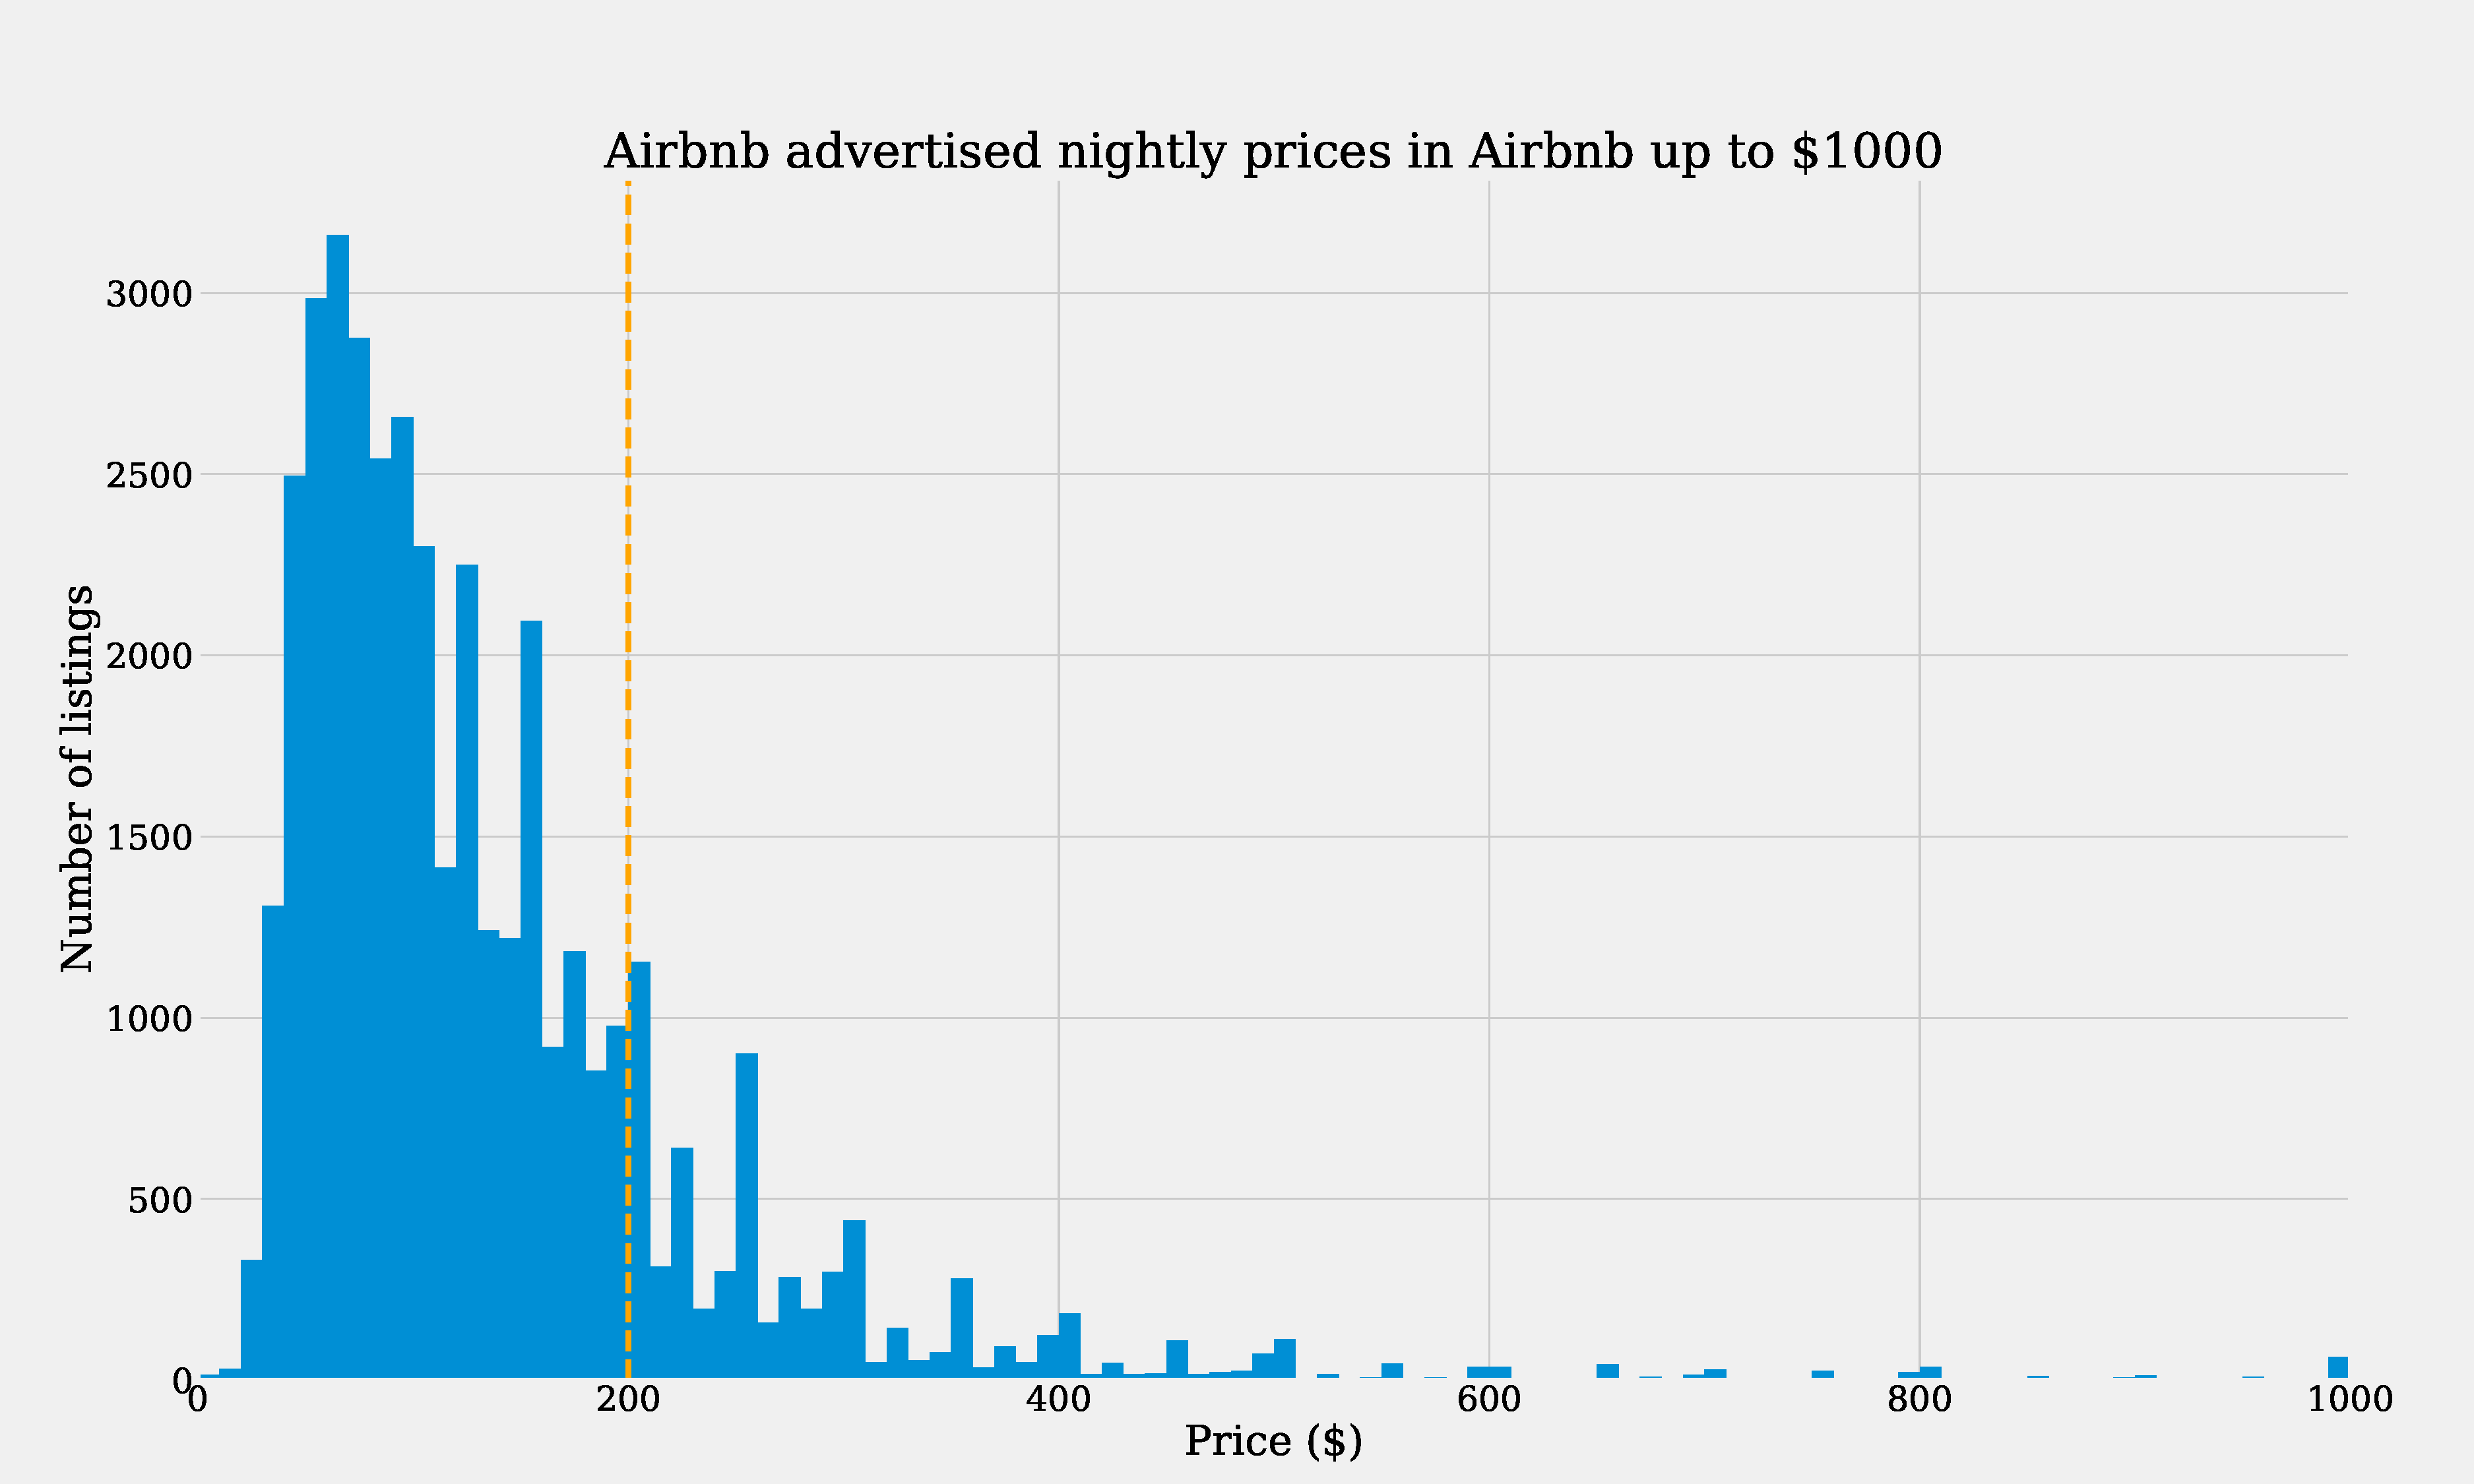
\includegraphics[width=\textwidth]{price-distribution-up-to-1000.pdf}
        \caption{Airbnb advertised price up to \$1000}
        \label{fig:price-distribution-1000}
\end{figure}

\begin{figure}[!htbp] \centering
    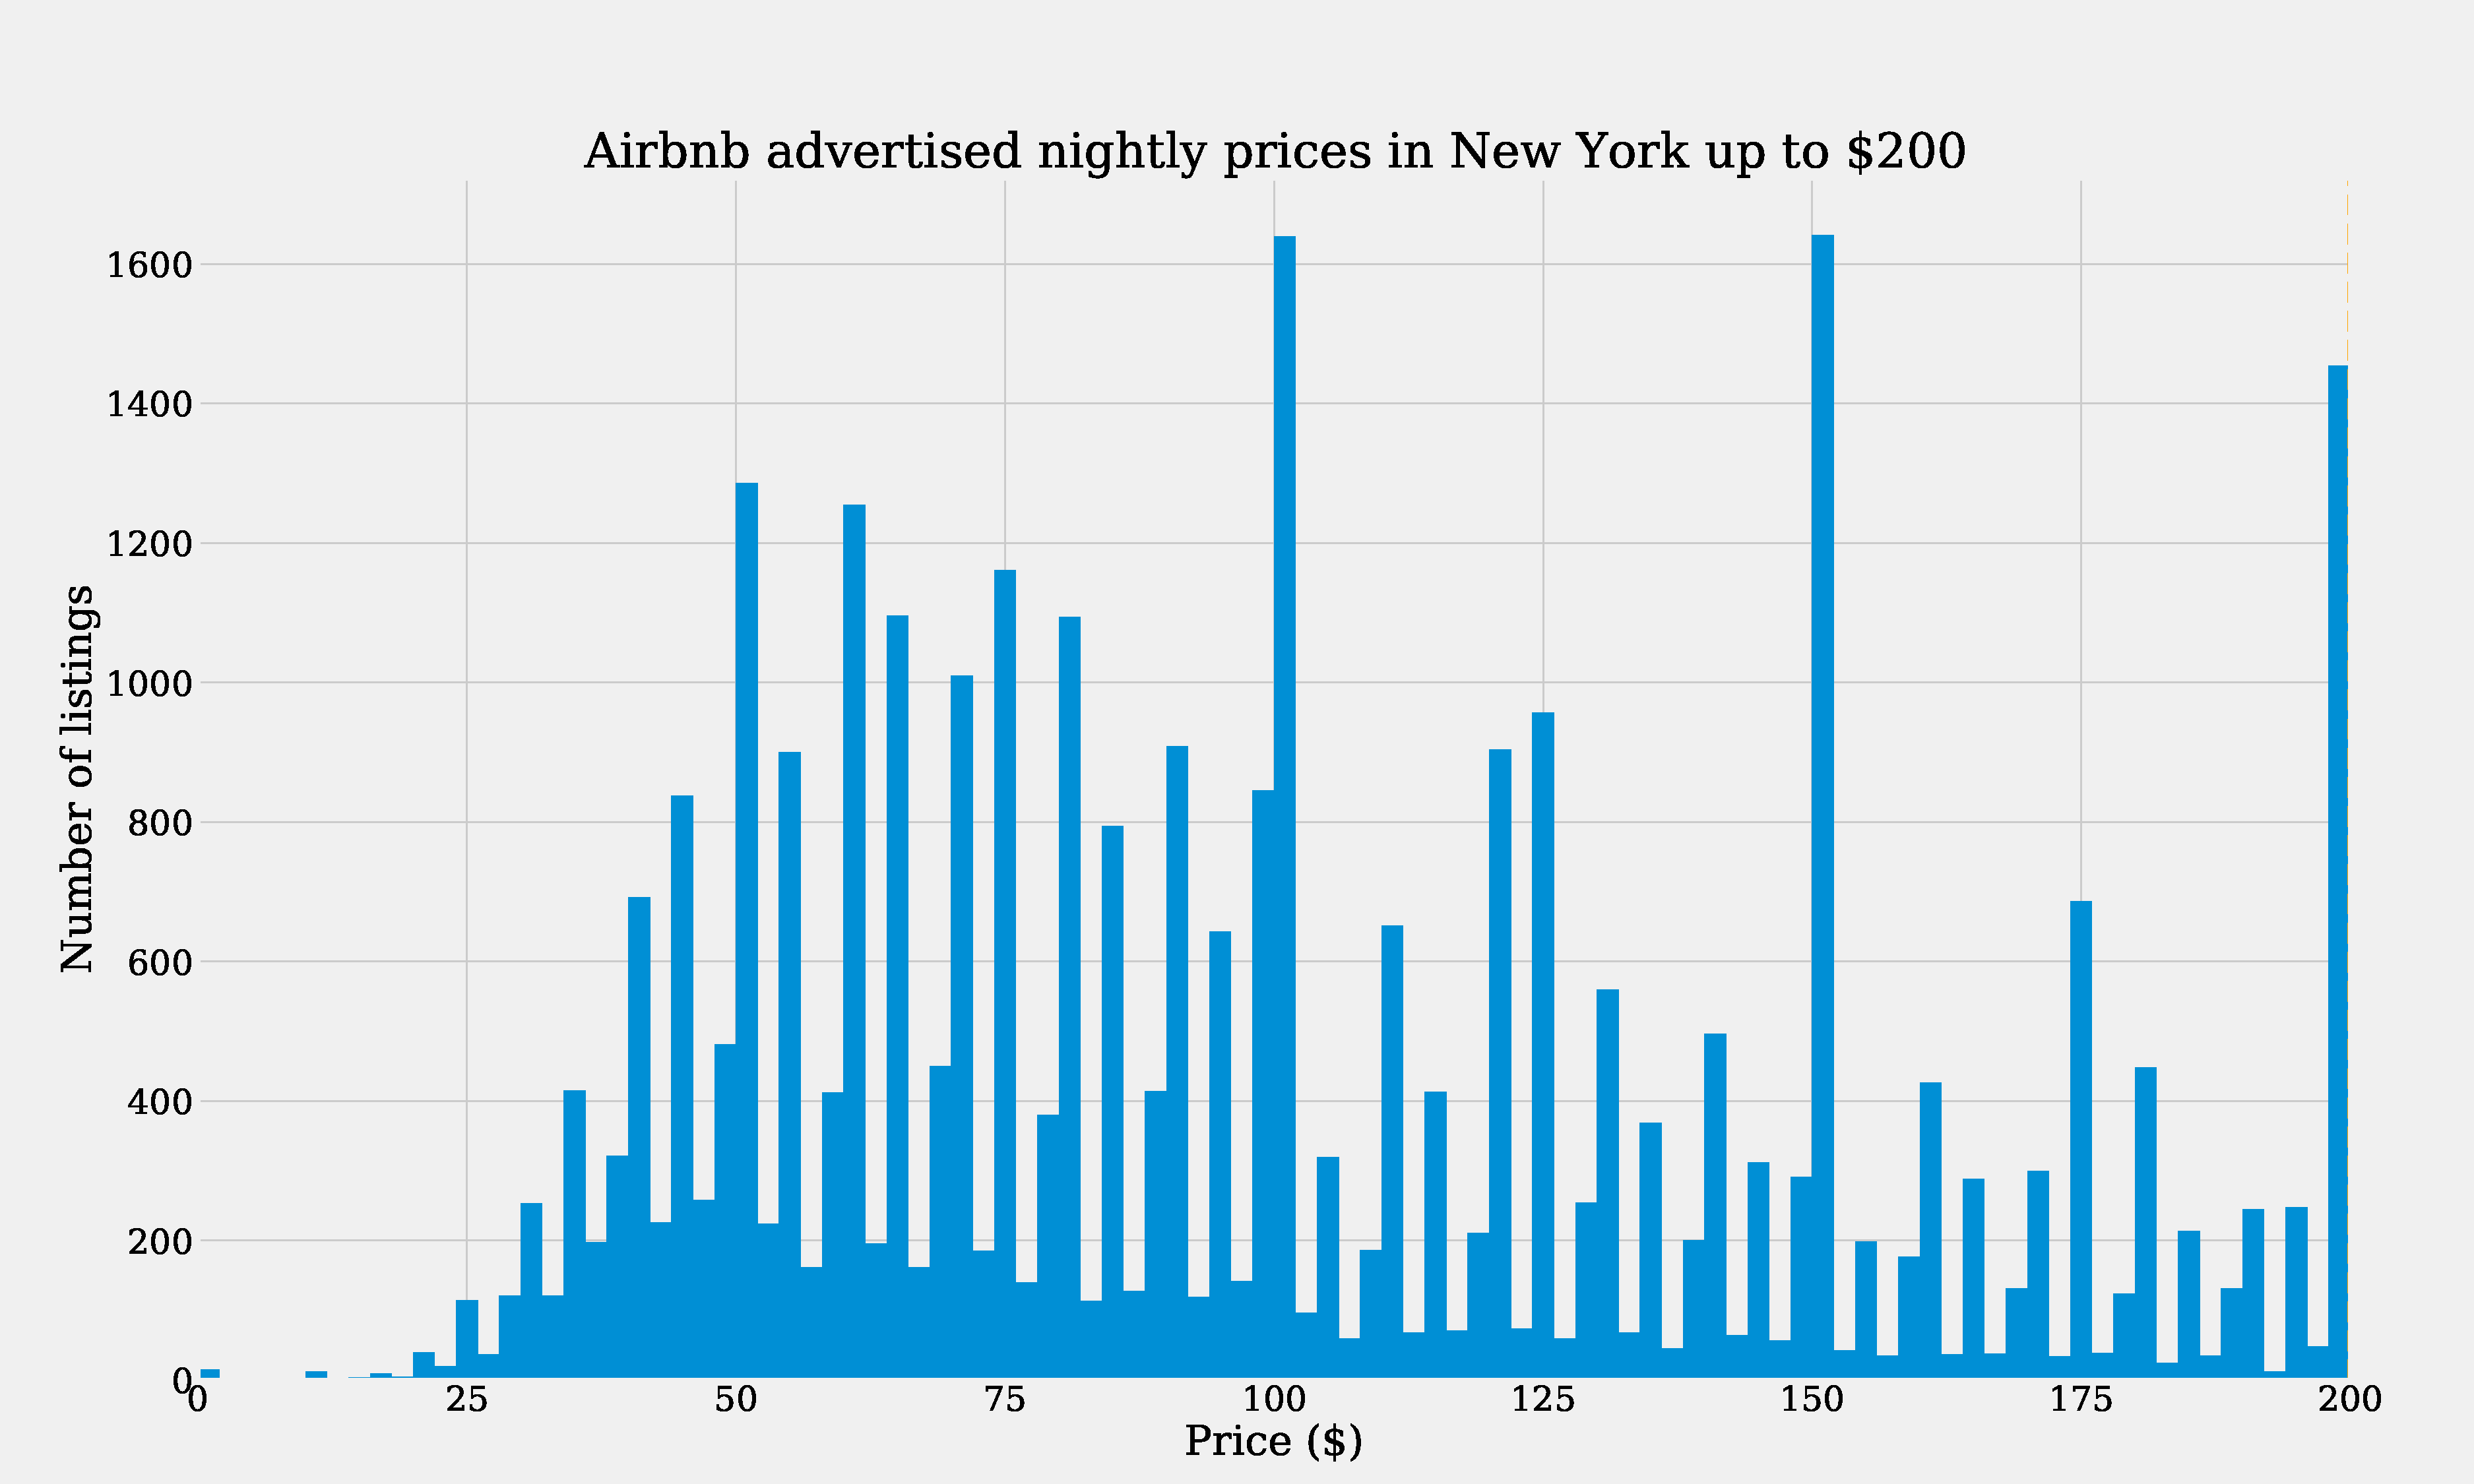
\includegraphics[width=\textwidth]{price-distribution-up-to-200.pdf}
        \caption{Airbnb advertised price up to \$200}
        \label{fig:price-distribution-200}
\end{figure}

\subsubsection*{Host Listings Count}

The median number of listings that the host of each listing has is 1. The mean
is higher (8 in total) due to some hosts running many listings. About 55\% of
listings are from hosts with one listing, and 45\% are from multi-listing hosts.
This feature has been shown to have a positive effect on the price of Airbnb
listings(\cite{chen2017consumer}, \cite{ert2016trust}, \cite{wang2017price})

\subsubsection*{Number of people accommodated, bathrooms, bedrooms and beds}

~\Cref{fig:accommodates-countplot,fig:bathrooms-countplot,fig:bedrooms-countplot,fig:beds-countplot}
  reveal that the most common listing type accommodates two people in one bed
  in one
bedroom with one bathroom.

The number of bedrooms, number of bathrooms, and number of accommodations appear
to have a positive impact on Airbnb rental price (\cite{ert2016trust};
\cite{chen2017consumer}; \cite{wang2017price}; \cite{gibbs2018use}). Figures
\ref{fig:median-price-by-accommodates} - ~\ref{fig:median-price-by-beds} show that the more people a listing
accommodates, the more number of bedrooms it has, the more bathrooms it has, the
higher the price they can charge their customers. However, we can see that those
figures' general trends are similar, which implies that those features may be
highly correlated.

\subsection{Categorical features}
\label{sec:categorical_features}

Our main EDA objective for categorical data is to know the unique values and
their corresponding count.

\subsubsection*{Neighbourhood}
\label{eda:neighbourhood}

Several numbers of published studies recognize the importance of locational
factors in the pricing strategy of Airbnb.  A listing close to the city center
(\cite{gibbs2018use};\cite{li2016pros}; \cite{wang2017price};
\cite{zhang2017key};\cite{gibbs2018use}) and coastline (\cite{perez2018and}) has
a higher room rate.  \cite{perez2018and} also found that a listing located
within sightseeing, eating, or shopping area gains a price premium.

As shown in Figure \ref{fig:borough-number-of-listing} and Figure
\ref{fig:borough-price-distribution}, Manhattan and Brookly have most Airbnb
properties are the most expensive boroughs, which is not surprising because they
are the famous tourist attractions.  In those two boroughs, tourists can find
neighborhoods for almost any interest. For example:

\begin{itemize}
  \item Sightseeing: Midtown is the heart of New York shopping and theater and
    home to some of its most iconic buildings.
  \item Nightlife:  More clubs are found in “Hell’s Kitchen,”
  \item Food: In Soho, tourists can experience a host of the highest-rated
    dining places.
  \item Theather: There is no more convenient home base than
    the Theater District,  located in 42nd Street to 50th Street west of Sixth
    Avenue.
  \item For families: Upper West Side is bordered with parks and playgrounds and
  boasting both a children’s museum and the famed dinosaurs at the American Museum
  of Natural. This neighborhood is also considered one of the safest areas of New
  York City
\end{itemize}


\begin{figure}[!htbp] \centering
  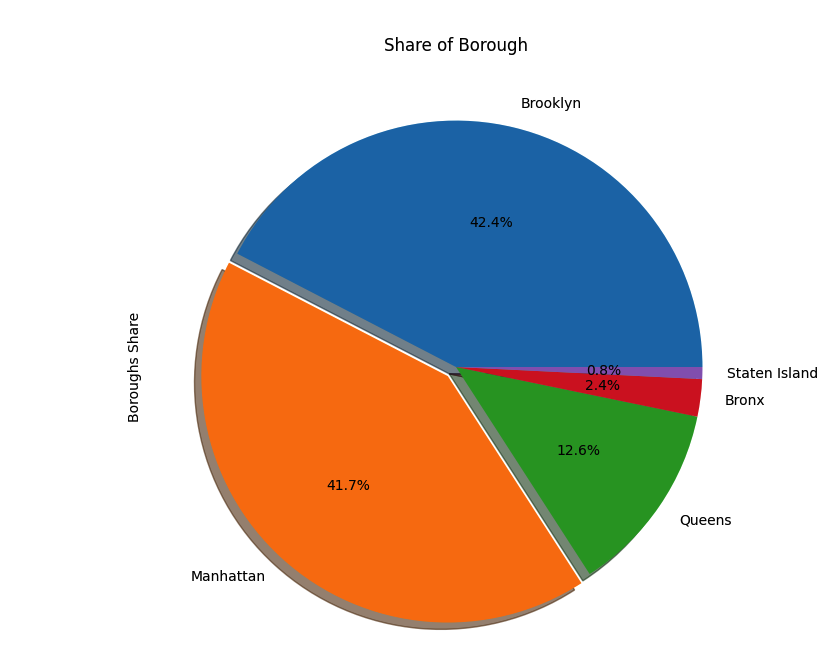
\includegraphics[width=0.9\textwidth]{share-of-borough.png}
    \caption{Borough Listings}
    \label{fig:borough-number-of-listing}
\end{figure}


\begin{figure}[!htbp]\centering
    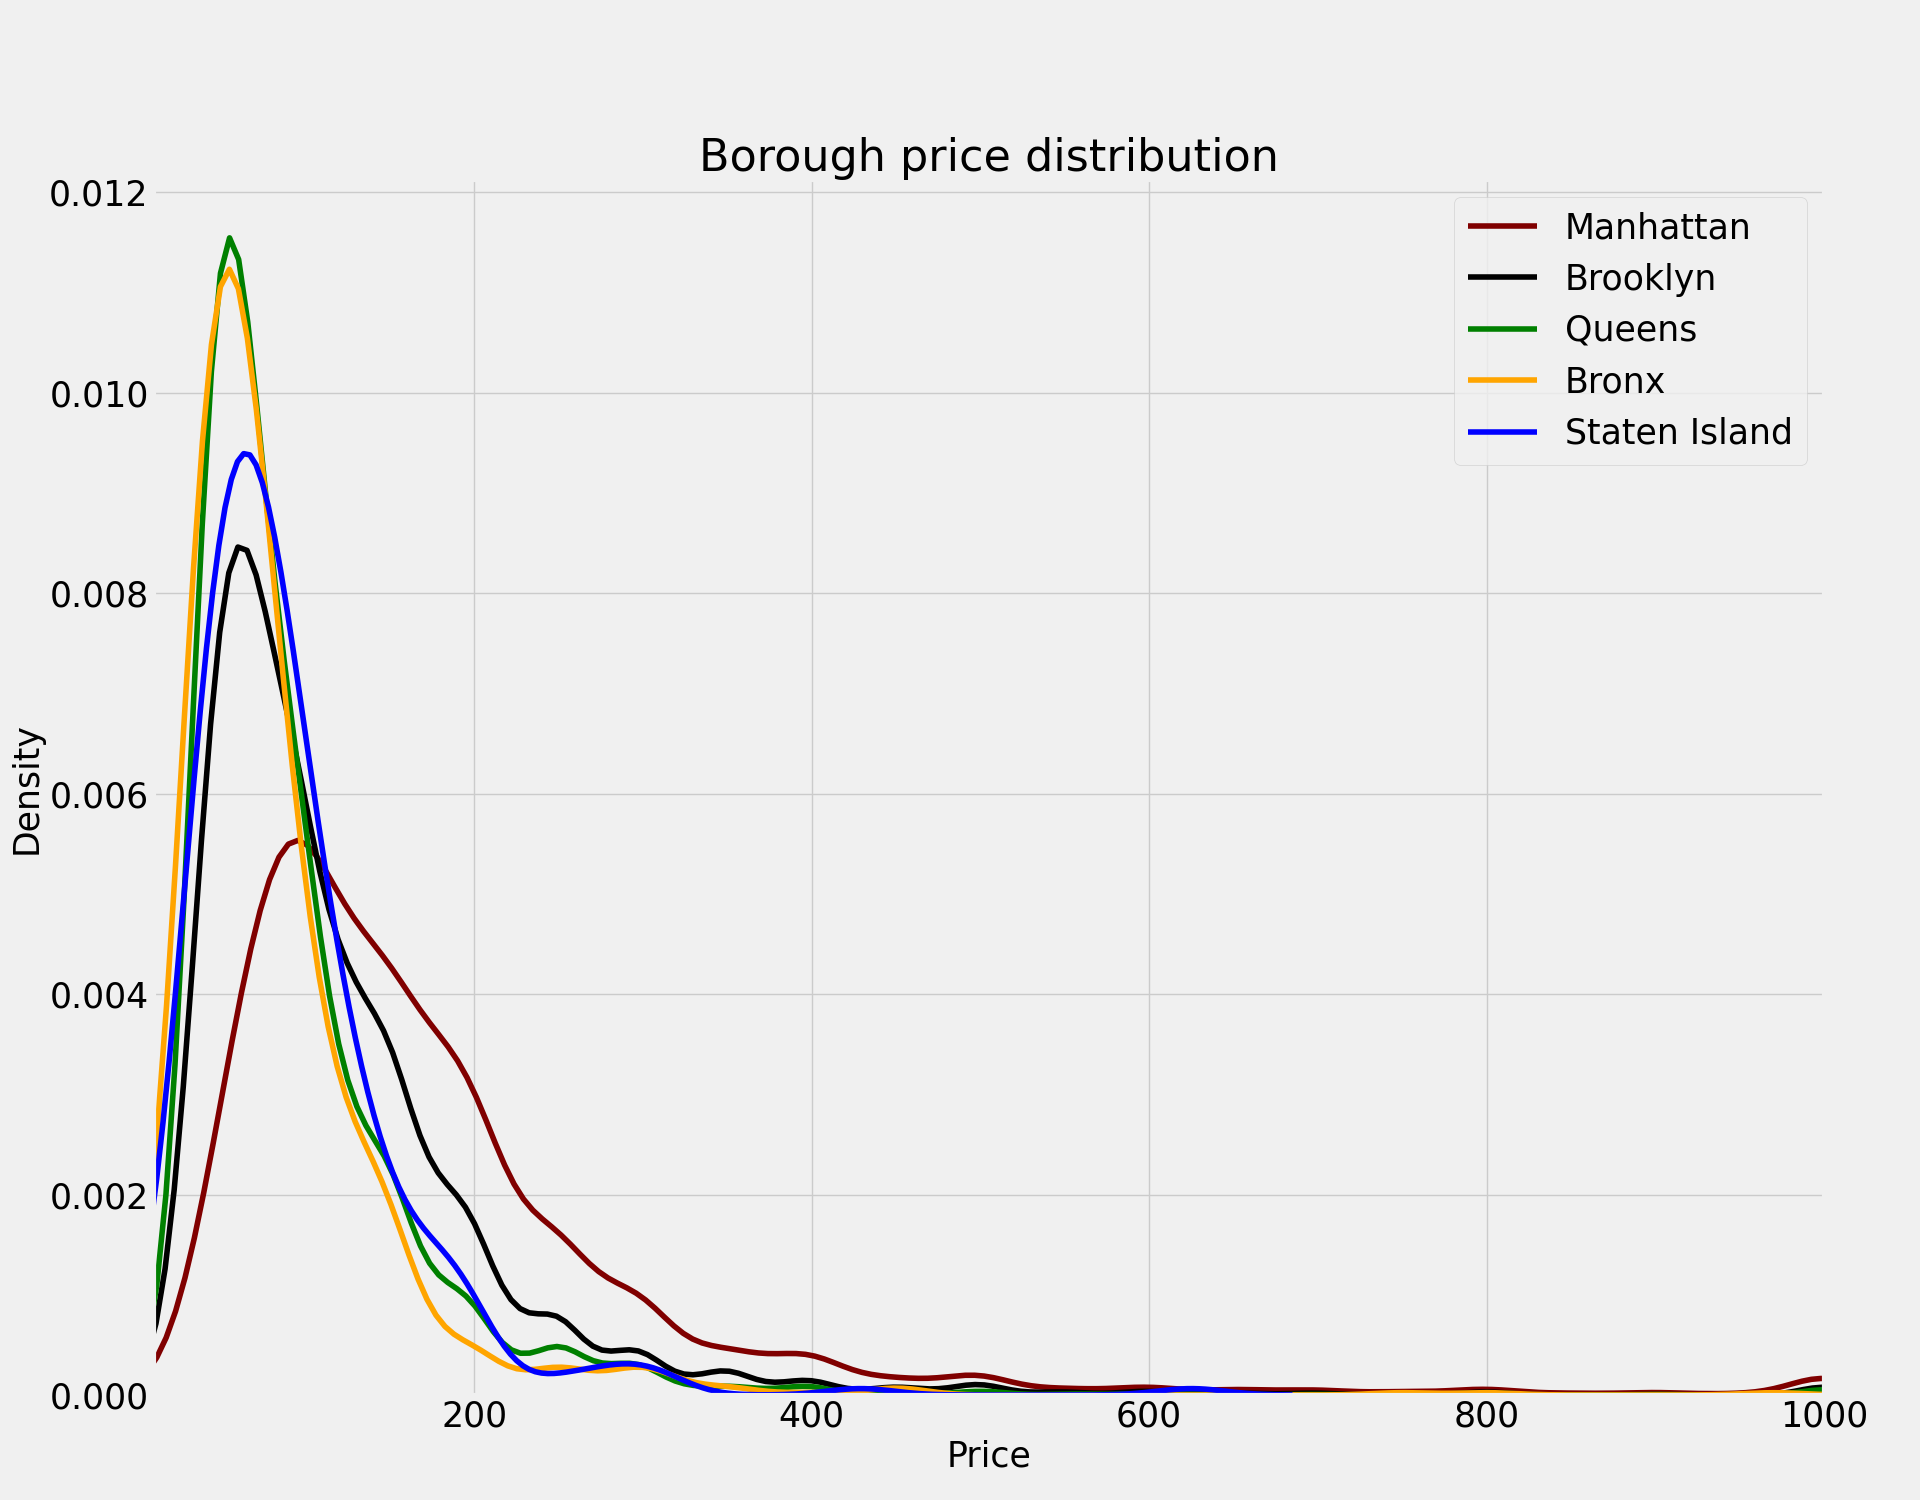
\includegraphics[width=0.9\textwidth]{borough-price-distribution.png}
    \caption{Borough Price Distribution}
    \label{fig:borough-price-distribution}
\end{figure}

\subsubsection*{Property and room types}

As shown in Figure \ref{fig:property_type},
about 80\% properties are apartments. The remainder are houses or more uncommon
property types (e.g. 'bed and breakfast' or 'yurt'). The median price of
apartment type listing is higher than that of house type listing but lower than
uncommon property types (\ref{fig:property_type_price}).

\begin{figure}[!htbp]
    \centering
        \centering
        \caption{Property Type Pie Chart}
        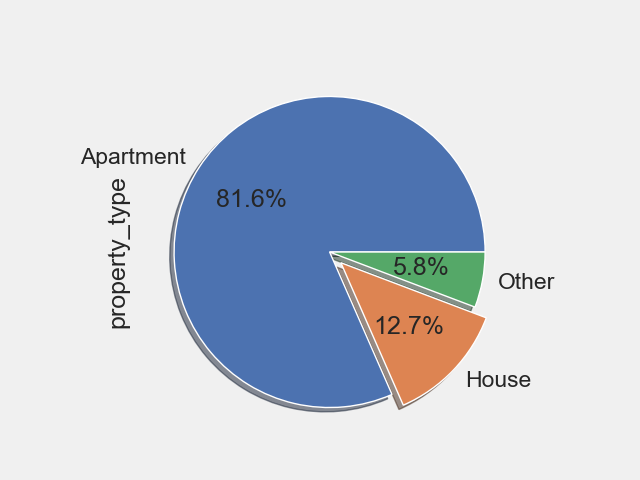
\includegraphics[width=0.7\textwidth]{Figure_12_property_type_pie.png}
      \label{fig:property_type}
\end{figure}

\begin{figure}[!htbp]
        \centering
        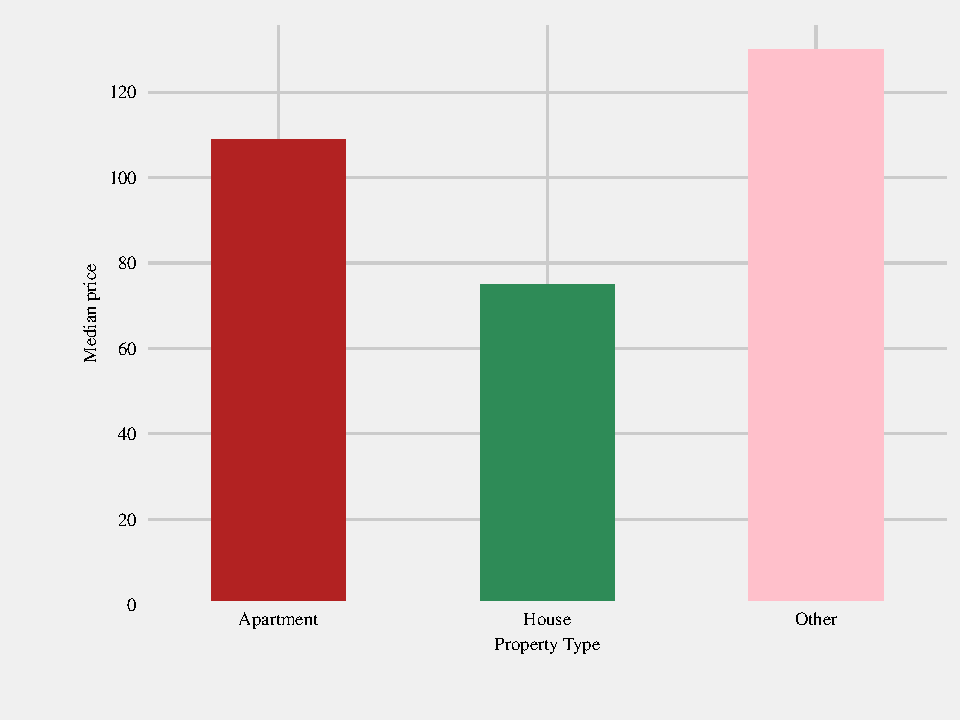
\includegraphics[width=0.85\textwidth]{median-price-by-property-type.pdf}
        \caption{Median Price By Property Type}
        \label{fig:property_type_price}
\end{figure}

Figure ~\ref{fig:room_type_pie} shows that about 52\% of listings are entire homes
(i.e. you are renting the entire property on your own). Most of the remainder
are private rooms (i.e. you are renting a bedroom and possibly also a bathroom,
but there will be other people in the property). Fewer than 3\% are shared rooms
(i.e. you are sharing a room with either the property owner or other guests).

On the question of whether there's a price difference between different types of
rooms, Figure \ref{fig:room_type_price} reveals that the rental price of the
entire home and a private room, and a hotel room is higher than the shared room.
This finding is consistent with many recent studies (\cite{cai2019price} ;
\cite{benitez2018flexible}; \cite{chen2017consumer}; \cite{gibbs2018use})

\begin{figure}[!htbp]
    \centering
        \centering
        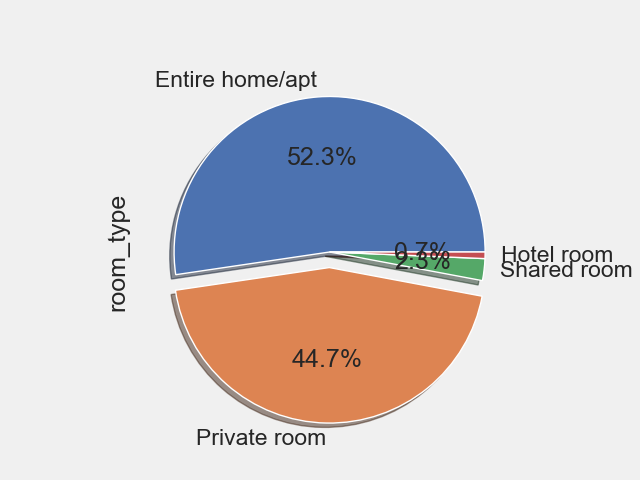
\includegraphics[width=0.7\textwidth]{Figure_12_room_type_pie.png}
        \caption{Room Type Pie Chart}
        \label{fig:room_type_pie}
\end{figure}

\begin{figure}[!htbp]
        \centering
        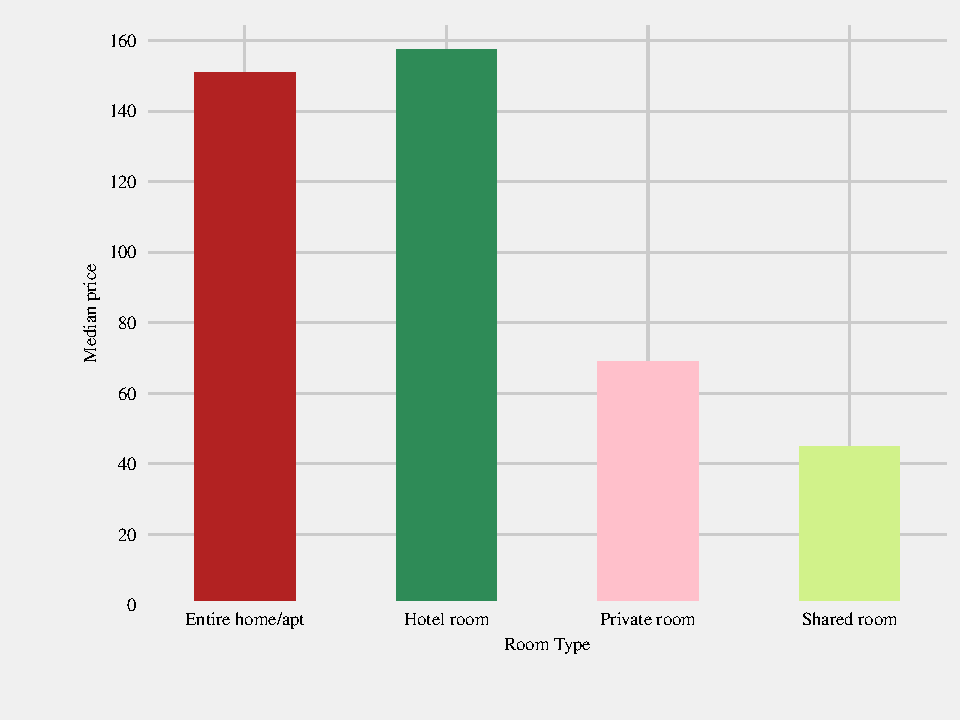
\includegraphics[width=0.85\textwidth]{median-price-by-room-type.pdf}
        \caption{Median Price By Room Type}
        \label{fig:room_type_price}
\end{figure}

\subsubsection*{Reviews}

From Figure   \ref{fig:overall-listing}, we see that, while few listings receive
review ratings of 80 or below, most listings with a review have received a
95-100/100 overall,  indicating that the customers adore their Airbnbs.


As shown in Figure \ref{fig:price_by_review_score_rating}, the review score
rating has a positive effect on the median rental price. It all makes intuitive
sense customers are willing to pay a premium price for a listing with a good
reputation.  However, the evidence for the relationship between is inconclusive.
Many studies (\cite{chen2017consumer}; \cite{gibbs2018use};
\cite{wang2017price}) have shown that the overall rating score has a positive
impact on rental price, while others (\cite{li2016pros}; \cite{zhang2017key})
suggests the otherwise.

\begin{figure}[!htbp]\centering
    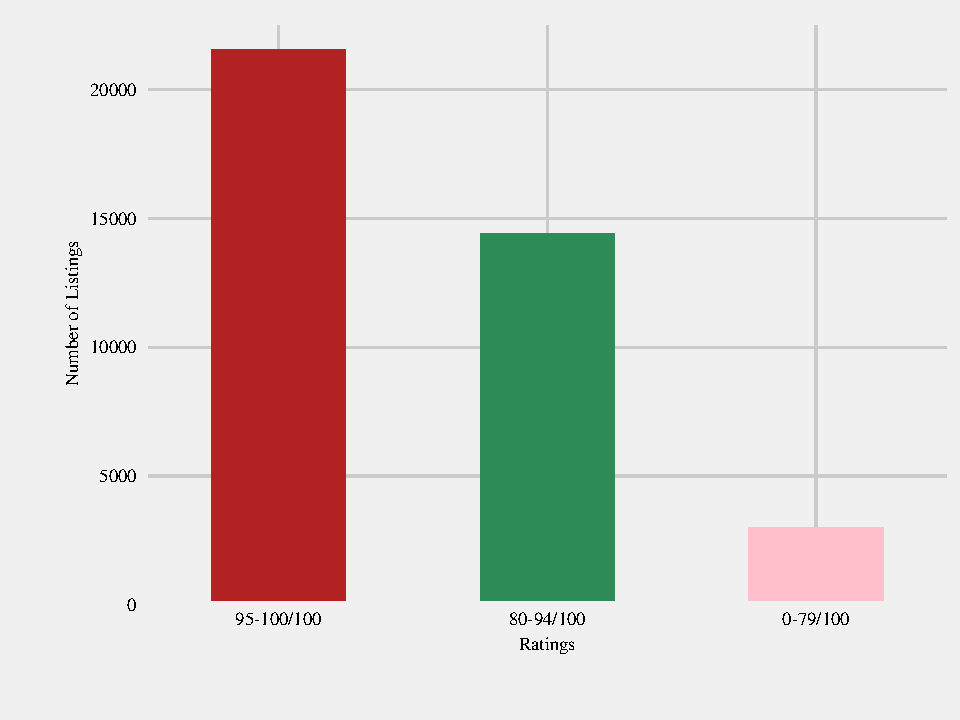
\includegraphics[width=0.85\textwidth]{review-rating-distribution.pdf}
    \caption{Overall Listing Rating Distribution}
    \label{fig:overall-listing}
\end{figure}

\begin{figure}[!htbp]\centering
    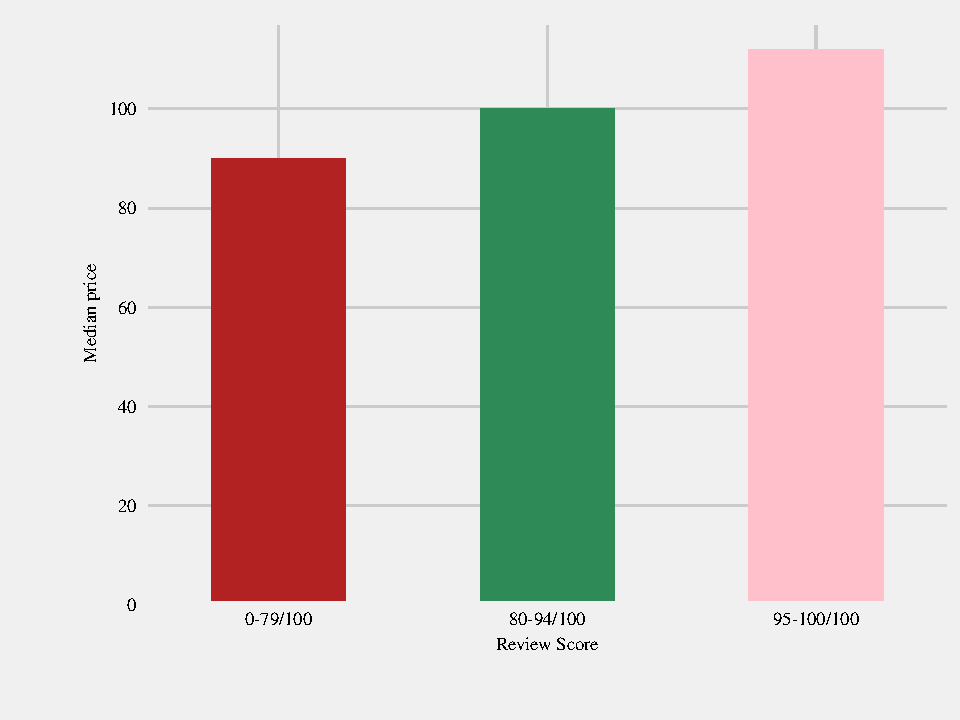
\includegraphics[width=0.85\textwidth]{median-price-by-reviews-rating.pdf}
    \caption{Median Price By Review Score Rating}
    \label{fig:price_by_review_score_rating}
\end{figure}

\subsubsection*{First and Last Review}

As can be seen from the Figure ~\ref{fig:time_since_first_review}, the most
common period in which  Airbnb listings had their first review is 2-3 years,
which means that many listings on the site have been active for at least a
couple of years. However,  fewer listings have been on Airbnb for more than four
years.

\begin{figure}[!htbp]\centering
    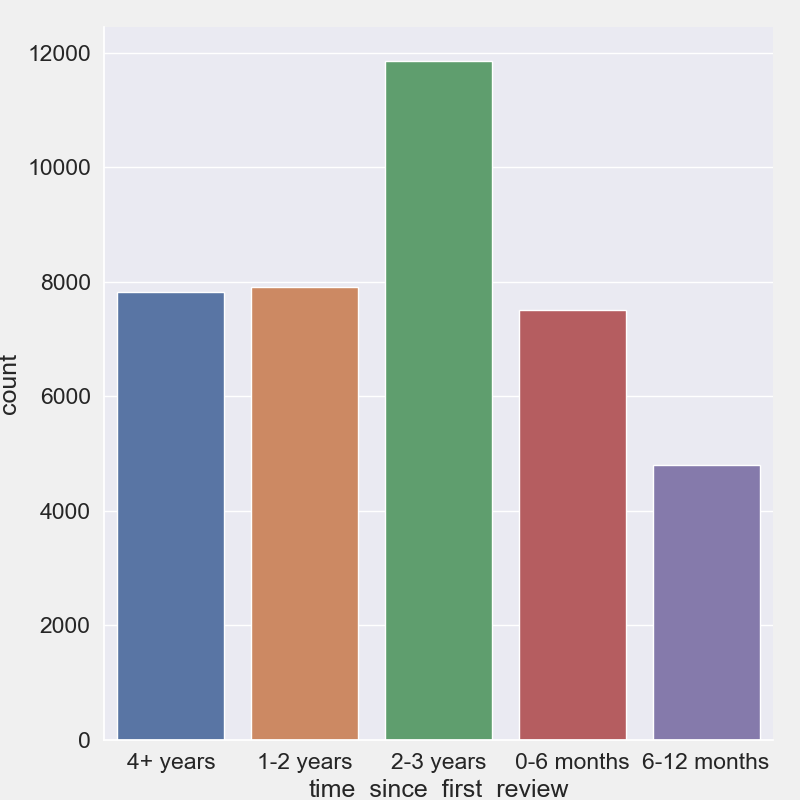
\includegraphics[width=0.7\textwidth]{Figure_15_time_since_first_review.png}
    \caption{Time Since First Review}
    \label{fig:time_since_first_review}
\end{figure}

We expect that people would pay a higher price for listing lives in Airbnb for a
long time than listings with a recent history with Airbnb.
While the rental price is higher for listings had their reviews for four years
or more, there's no difference in median price for other categories
(Figure \ref{fig:time_since_first_review_price})

\begin{figure}[!htbp]\centering
    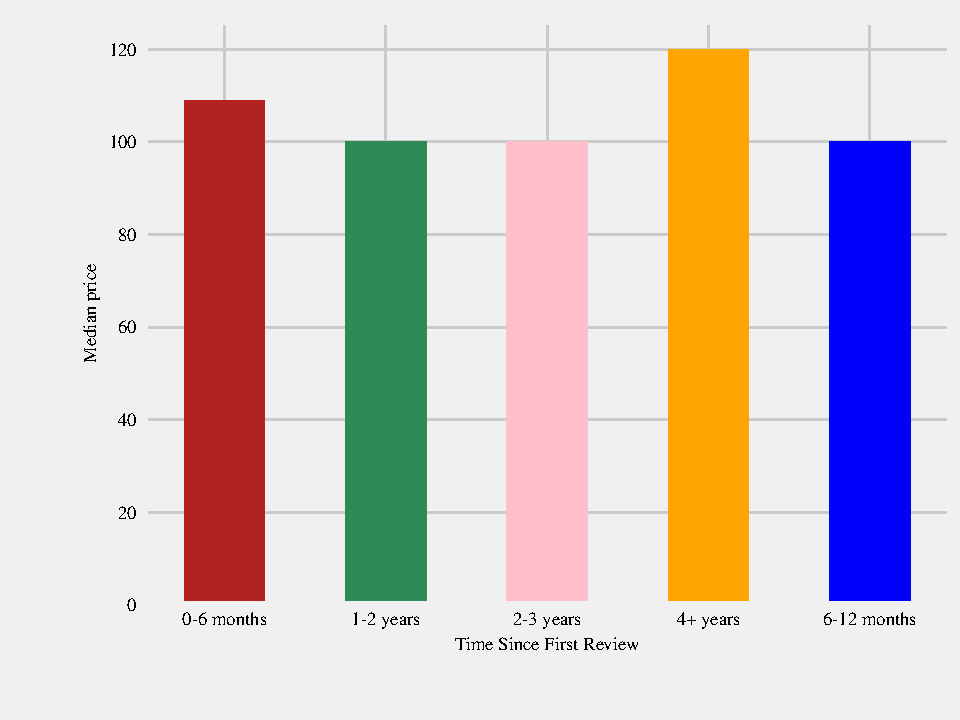
\includegraphics[width=0.9\textwidth]{median-price-by-time-since-first-review.pdf}
    \caption{Median Price By Time Since First Review}
    \label{fig:time_since_first_review_price}
\end{figure}

The bar plot ~\ref{fig:time_since_last_review} reveals that the most
common period since a listing received its last review is 2-8 weeks, which means
that many listings have been reviewed relatively recently.  What stands out in
the figure is that over 10,000 listings have not had a review for more than a
year, which means they exist on the site, but they do not have their calendars
open and are not available to reserve.

\begin{figure}[!htbp]\centering
    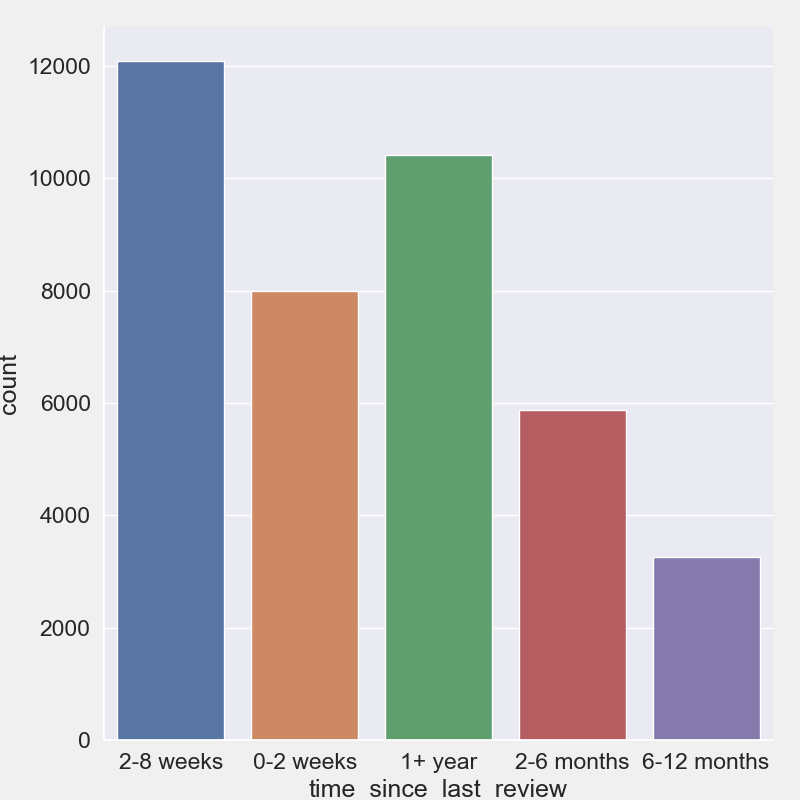
\includegraphics[width=0.7\textwidth]{Figure_15_time_since_last_review.png}
    \caption{Time Since Last Review}
    \label{fig:time_since_last_review}
\end{figure}

Time since the last review may have been an essential factor in how people
decide to rent an Airbnb listing. People may avoid booking accommodation that
has not been reviewed for a long time. Therefore, we expect the time since the
last review has a negative effect on the rental price. Contrary to our
expectation, Figure \ref{fig:time_since_last_review_price} showed no significant
difference between different categories of the number of days since the last
review.

\begin{figure}[!htbp]\centering
    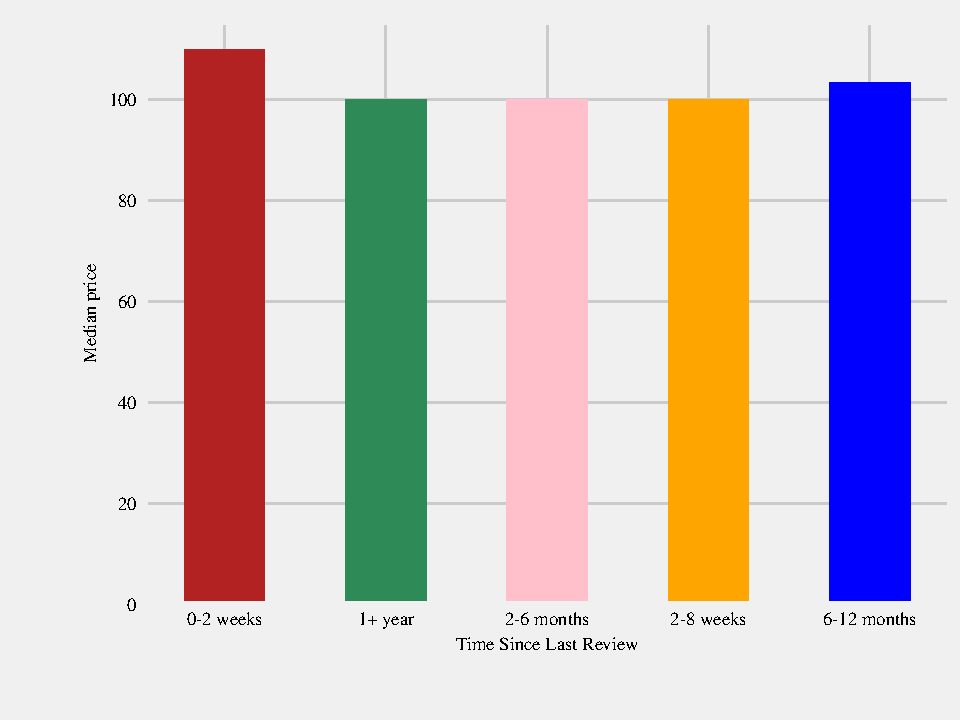
\includegraphics[width=0.9\textwidth]{median-price-by-time-since-last-review.pdf}
        \caption{Median Price By Time Since Last Review}
        \label{fig:time_since_last_review_price}
\end{figure}

\subsection{Boolean features}
\label{sec:boolean_features}

Many features (e.g. for amenities) can be true or false. This section compares
the proportions of these features that are true or false (to explore the data
and also to ascertain whether the feature is worth retaining), and the median
price of each category (to explore the relationship between the category and
price).

\subsubsection*{Superhosts}

Figure ~\ref{fig:host_is_superhost} shows that about 23\% of hosts have a
superhost badge. Hosts with superhost status usually charge higher prices. A
possible explanation for this might be that people are willing to pay a premium
price because they consider superhost status a mark of quality.  This also
accords with earlier studies(\cite{gibbs2018use},
\cite{kakar2016effects};\cite{wang2017price},\cite{cai2019price}).

\begin{figure}[!htbp]\centering
    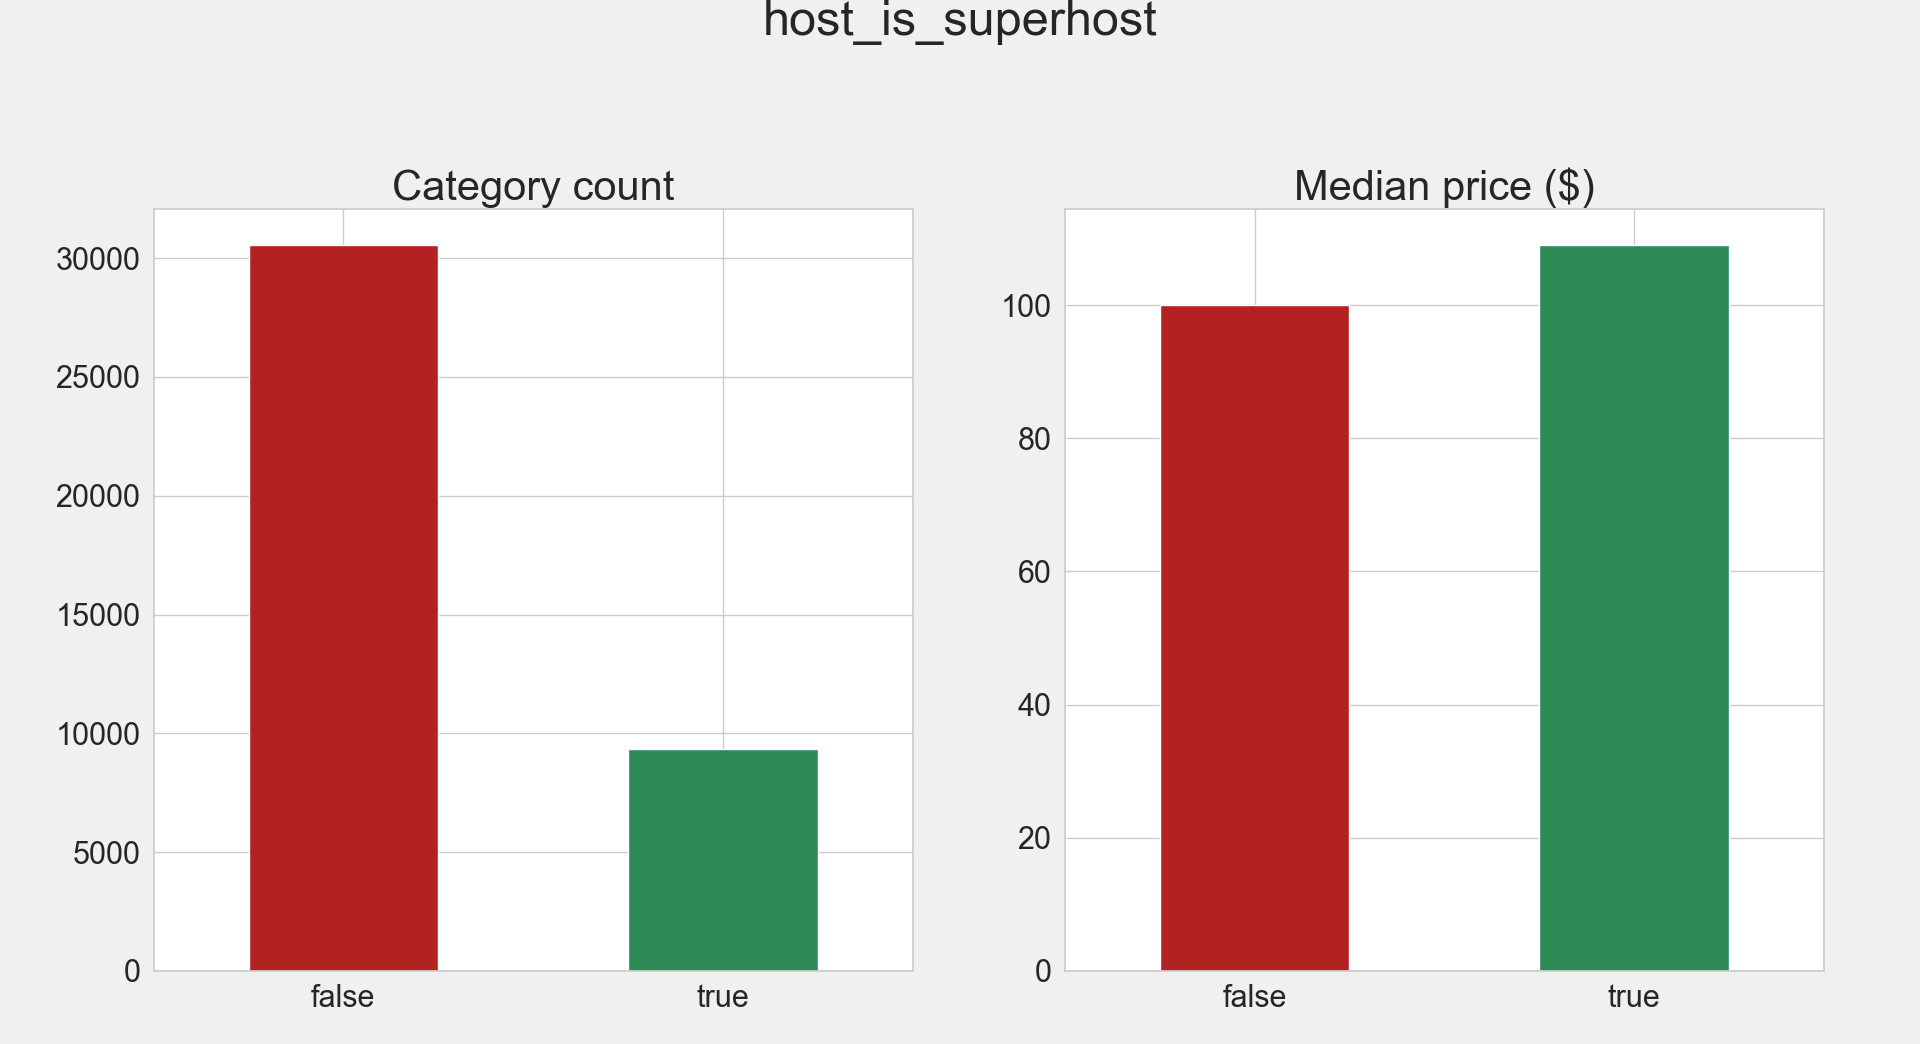
\includegraphics[width=\textwidth]{host-is-superhost.png}
    \caption{Count Plot and Median Price By Whether A Host Is a Superhost}
    \label{fig:host_is_superhost}
\end{figure}

\subsubsection*{Host verification}
In Figure ~\ref{fig:host_identity_verified}, about 49\% of hosts are verified.
Consistent with the literature (\cite{chen2017consumer}; \cite{wang2017price}),
the figure showed that hosts with verified profiles gain a price premium. The
relationship may be explained by the fact that verified profiles (e.g., by
providing ID and verifying your phone number and email address)  can increase
their trustworthiness and, therefore, can charge a higher rental price.

\begin{figure}[!htbp]\centering
    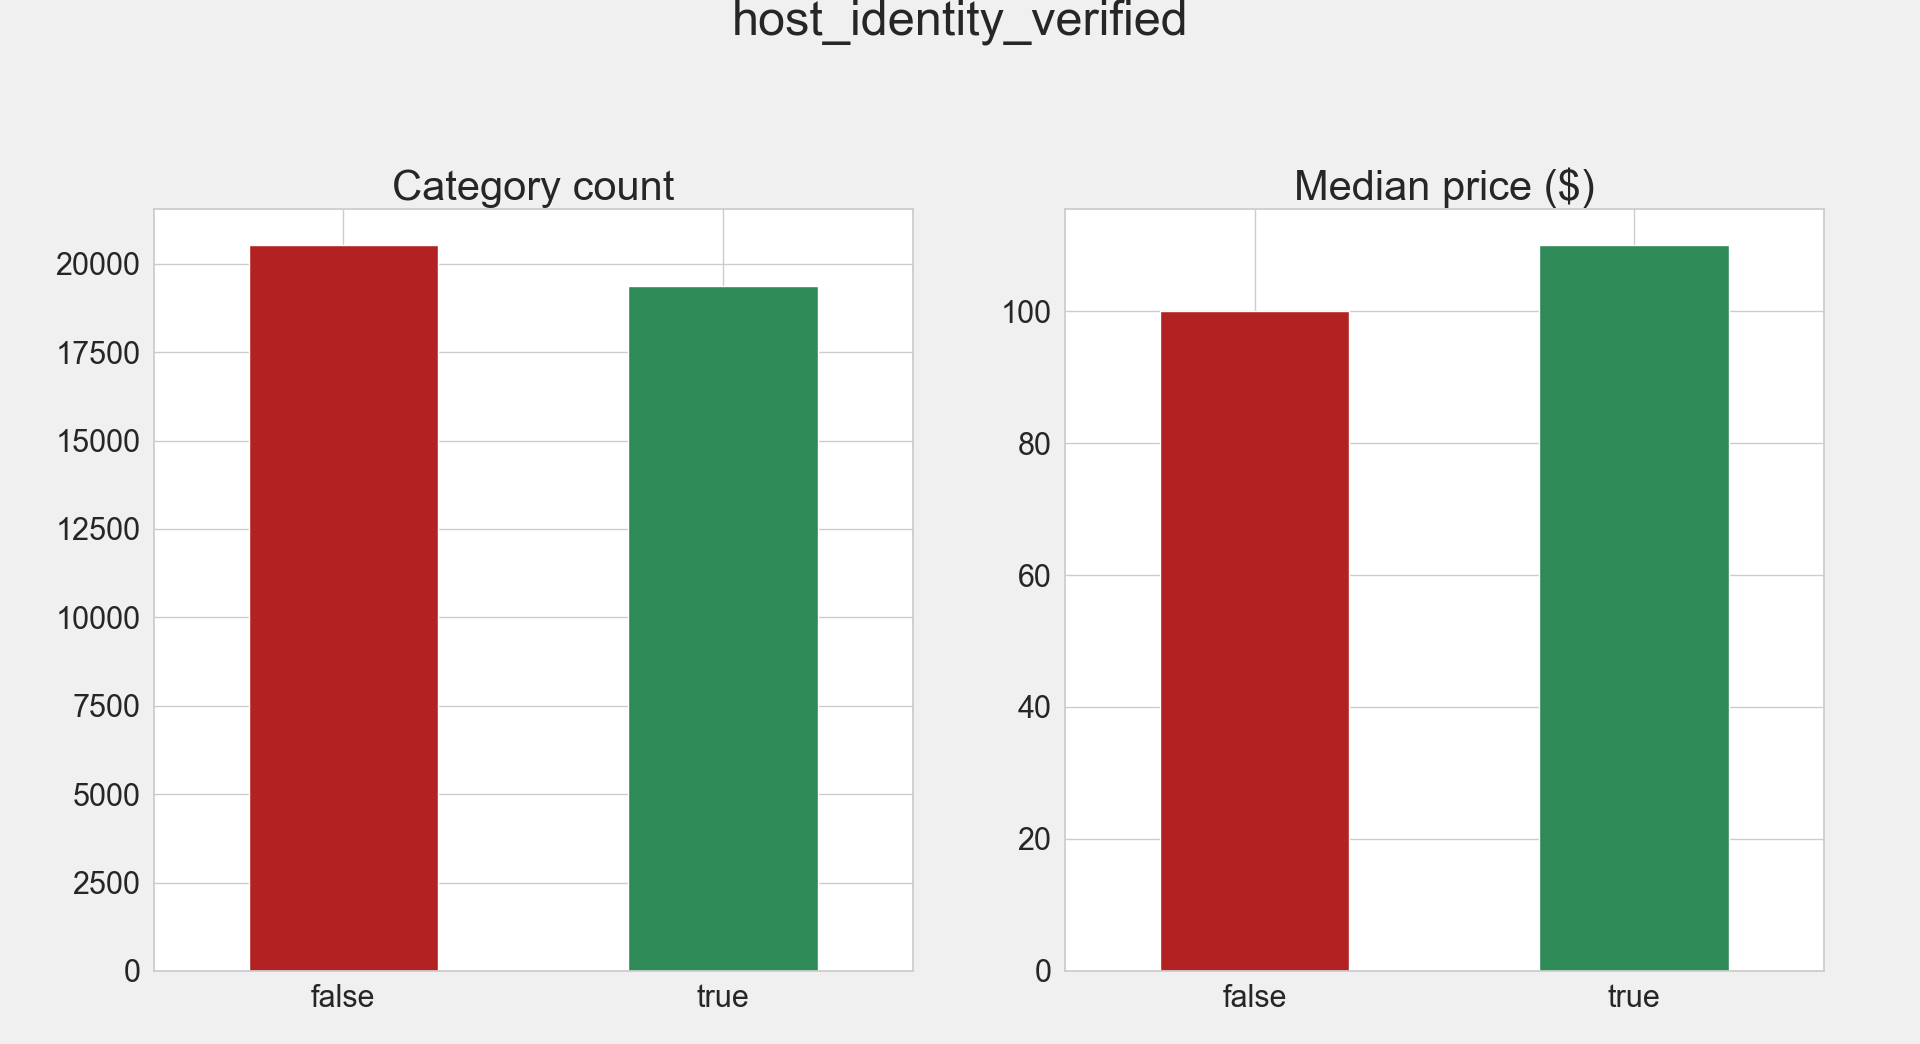
\includegraphics[width=\textwidth]{host-identity-verified.png}
    \caption{Count Plot and Median Price By Whether A Host Is Verified}
    \label{fig:host_identity_verified}
\end{figure}

\subsubsection*{Instant booking}

As shown in figure below, about 40\% of properties are instant bookable and
hosts that allow for immediate booking without confirmation  have lower prices
than those who do not. This finding seems counterintuitive, as we would expect
higher willingness-to-pay from potential guests for the added convinience of
intant booking.  This negative link can be explained by both emotional
(\textcite{wang2017price}) and economic (\textcite{benitez2018flexible}).

\begin{figure}[!htbp]
    \centering
    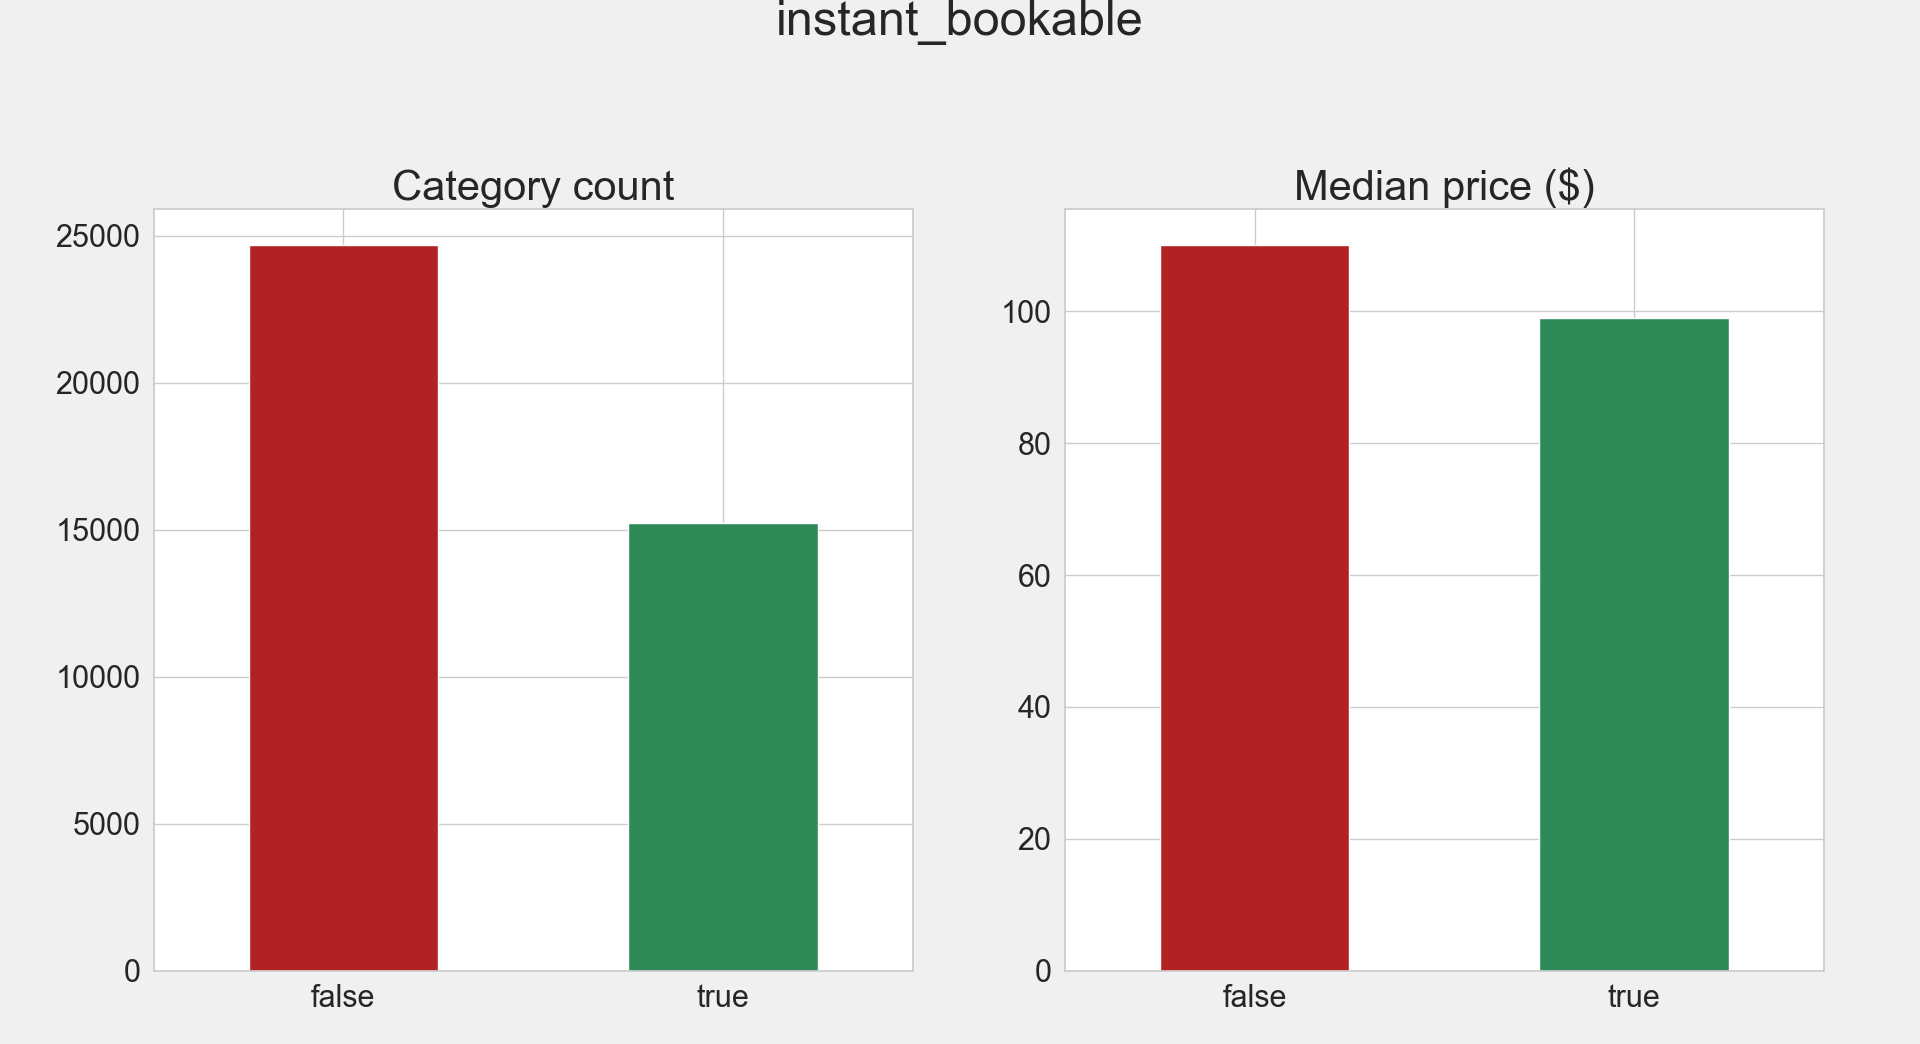
\includegraphics[width=\textwidth]{instant-bookable.png}
    \caption{instant\_bookable}
    \label{fig:instant_bookable}
\end{figure}

\subsubsection*{Amenities}

Our goal is to identify which amenities are common and which increase the price
of an Airbnb listing. We plot the count plot and each amenity's
median price to explore the relationship between the amenity and price.
Amenities then can be split into three groups:

\begin{enumerate}

  \item The first group contains uncommon amenity, but listings with it have a
    higher median price: Bed linen, Coffee machine, Basic cooking equipment,
    Elevator, Child friendly, Long term stays allowed, Private entrance, Self
    check-in, Pets allowed, Washer,dryer and/or dishwasher (white goods)
    (See
    ~\Cref{fig:elevator-and-bed-linen,fig:white-goods-and-pets-allowed,fig:self-checkin-and-coffee-machine,fig:long-term-stays-and-child-friendly,fig:private-entrance-and-cooking-basics})

  \item The second group includes common amenities and listings with it have a
      higher median price: TV, Internet, Air conditioner (See
      ~\Cref{fig:tv-and-internet,fig:air-conditioner}).

  \item The third group comprises uncommon amenities, and listings with it have
      a lower median price:  free car parking (presumably because these are less
      likely to be central properties), greeted by host. (See
      ~\Cref{fig:parking-and-host-greeting})

\end{enumerate}

It is somewhat surprising that free car parking does not have a significant
influence on the rental price. This may be because the more comfortable way and
quickest way to travel around New York City is by the subway, so people would
not consider car parking a critical factor when deciding to rent an Airbnb
listing. The reason why the host greeting does not associate with a higher price
is not apparent.

\subsection{Multivariate Exploration}
\label{sec:multivariate-exploration}

The goal of this section is to investigate the relationships between pairs of
our features. A primary concern when analyzing the relationship between various
variables is multicollinearity, a phenomenon in which two or more independent
variables substantially correlate(\textcite{cohen2013applied}).

While multicollinearity does not hurt the model's predictive
power(\textcite{kutner2005applied}), collinearity can pose problems in the
regression context. In particular,  it can be challenging to separate the
individual effects of collinear independent variables on the outcome variable.

A straightforward way to detect collinearity is to construct a correlation
matrix among predictors.  An element of this matrix that is large in absolute
value indicates a pair of highly correlated variables and are indicative of
collinearity issues.


As shown in Figure ~\ref{fig:correlation-matrix} shows the correlation matrix,
areas of multicollinearity are:
\begin{itemize}
    \item Beds, bedrooms, guests included, and the number of people that
      property accommodates are highly correlated.
    \item There are strong negative correlations between houses and apartments
        and between private rooms and entire homes.
\end{itemize}

Providing a full remedy for the multicollinearity issue is beyond the scope of
this thesis. However, we employ two  simple approaches as followed:

\begin{enumerate}
    \item The first approach is to drop problematic variables from the regression.
    \item The second method is to employ regularization techniques, which combat
        collinearity by using biased models (as demonstrated in section \ref{ssec:penalized_regression_models}),
        which reduce the error variance of estimators.
\end{enumerate}

\subsection{Time Series Analysis}
\label{sec:time_series}

We now also plotted time series charts to check for trends and seasonality.
First, we examine how long hosts have been listing properties on Airbnb in New
York.Of the Airbnb hosts that are active on the site, the first joined on 22
August 2008, and the most recent joined on 03 December 2019.
From 2011 onwards, the number of listings started growing considerably. However,
growth in the number of new hosts (of those currently listed on the site) has
decreased since mid-2014 (The trend curve in Figure
~\ref{fig:number_of_hosts_joining}).

Strong evidence of seasonality was found in  seasonal curve (Figure
~\ref{fig:number_of_hosts_joining}). The number of hosts joining Airbnb peaked in
the summer because people put properties online to utilize the increased number
of tourists in the summer holidays.


\begin{figure}[!htbp] \centering
    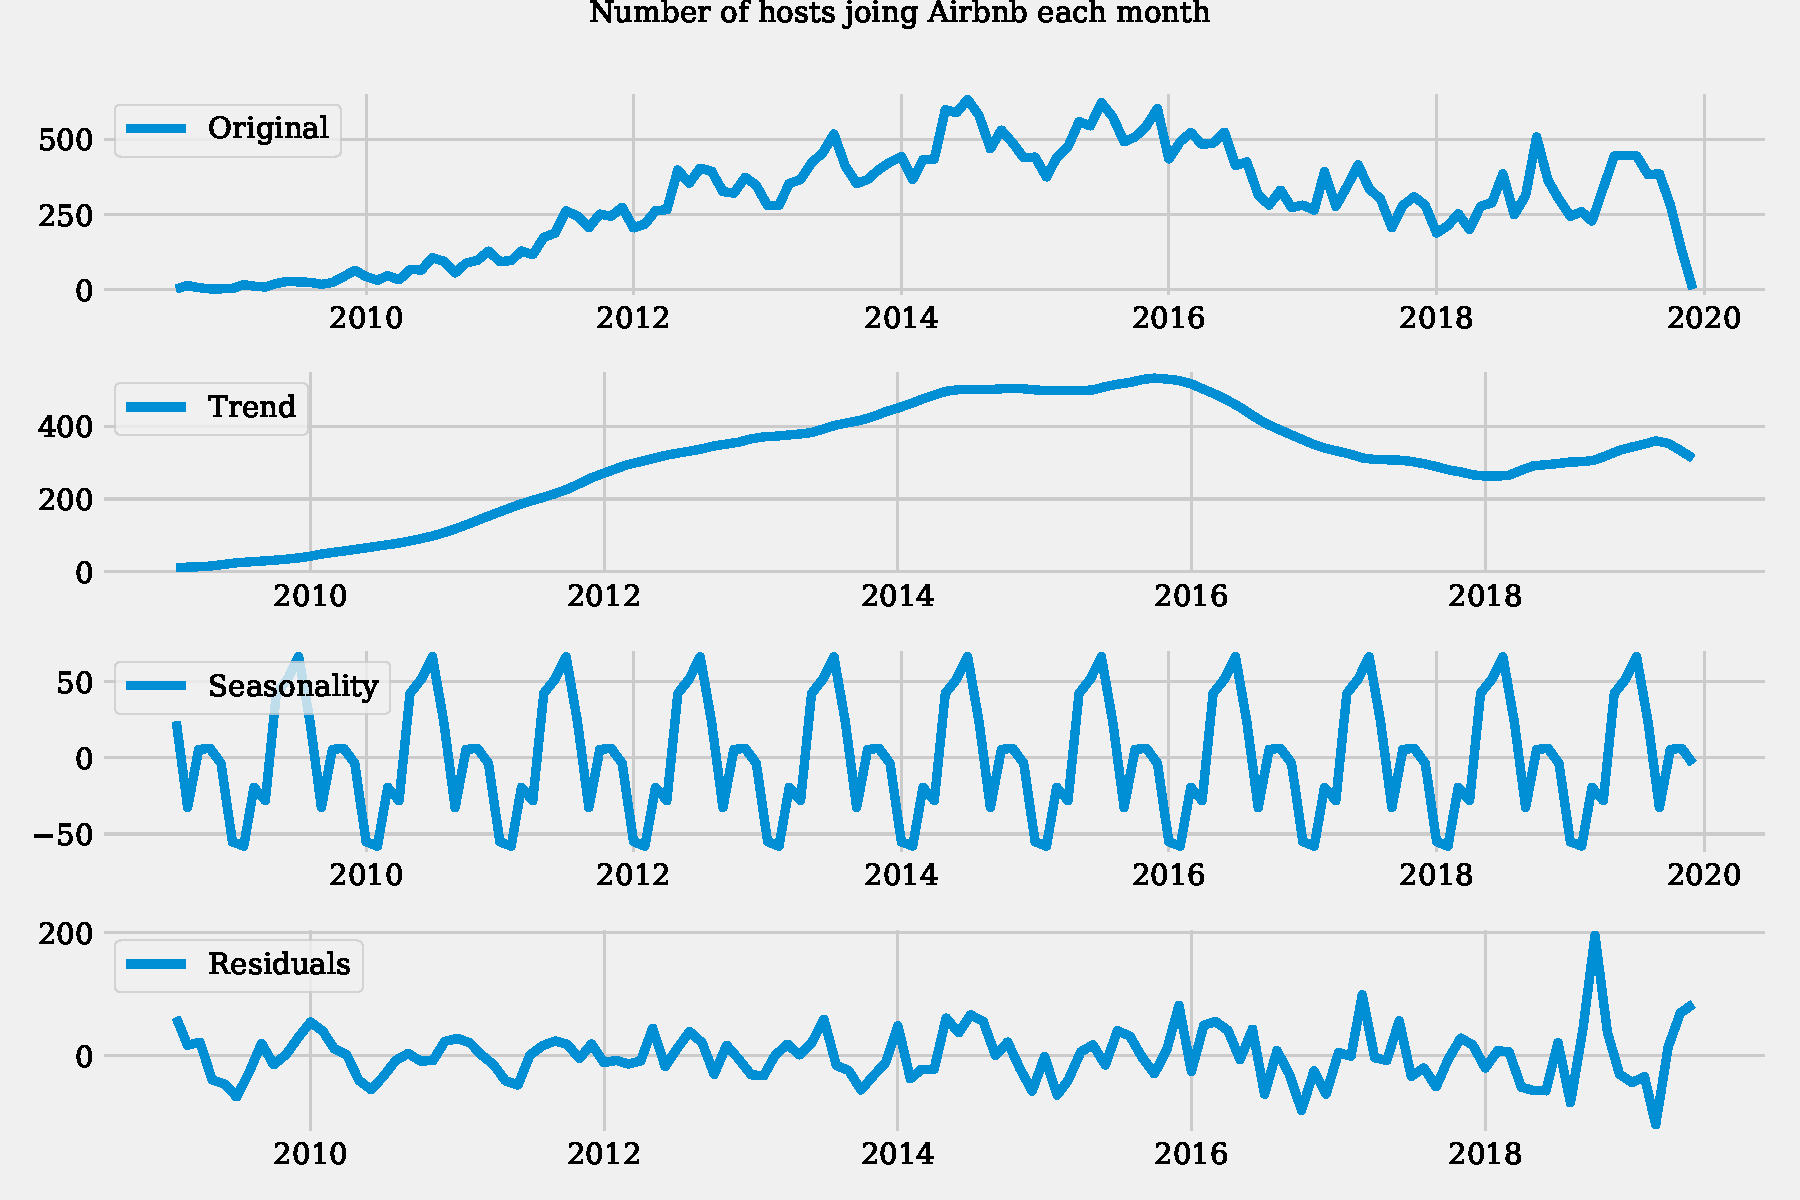
\includegraphics[width=\textwidth]{number-of-host-joining-each-month.pdf}
    \caption{Number of hosts joining Airbnb each month}
    \label{fig:number_of_hosts_joining}
\end{figure}

In terms of how prices changed over time, Figure
~\ref{fig:prices-change-by-years} shows that the average price per night for
Airbnb listings in New York has increased slightly over the
last ten years. Particularly, the top-tier property prices have increased,
resulting in a more substantial increase in the mean price than the median.


\begin{figure}[!htbp] \centering
    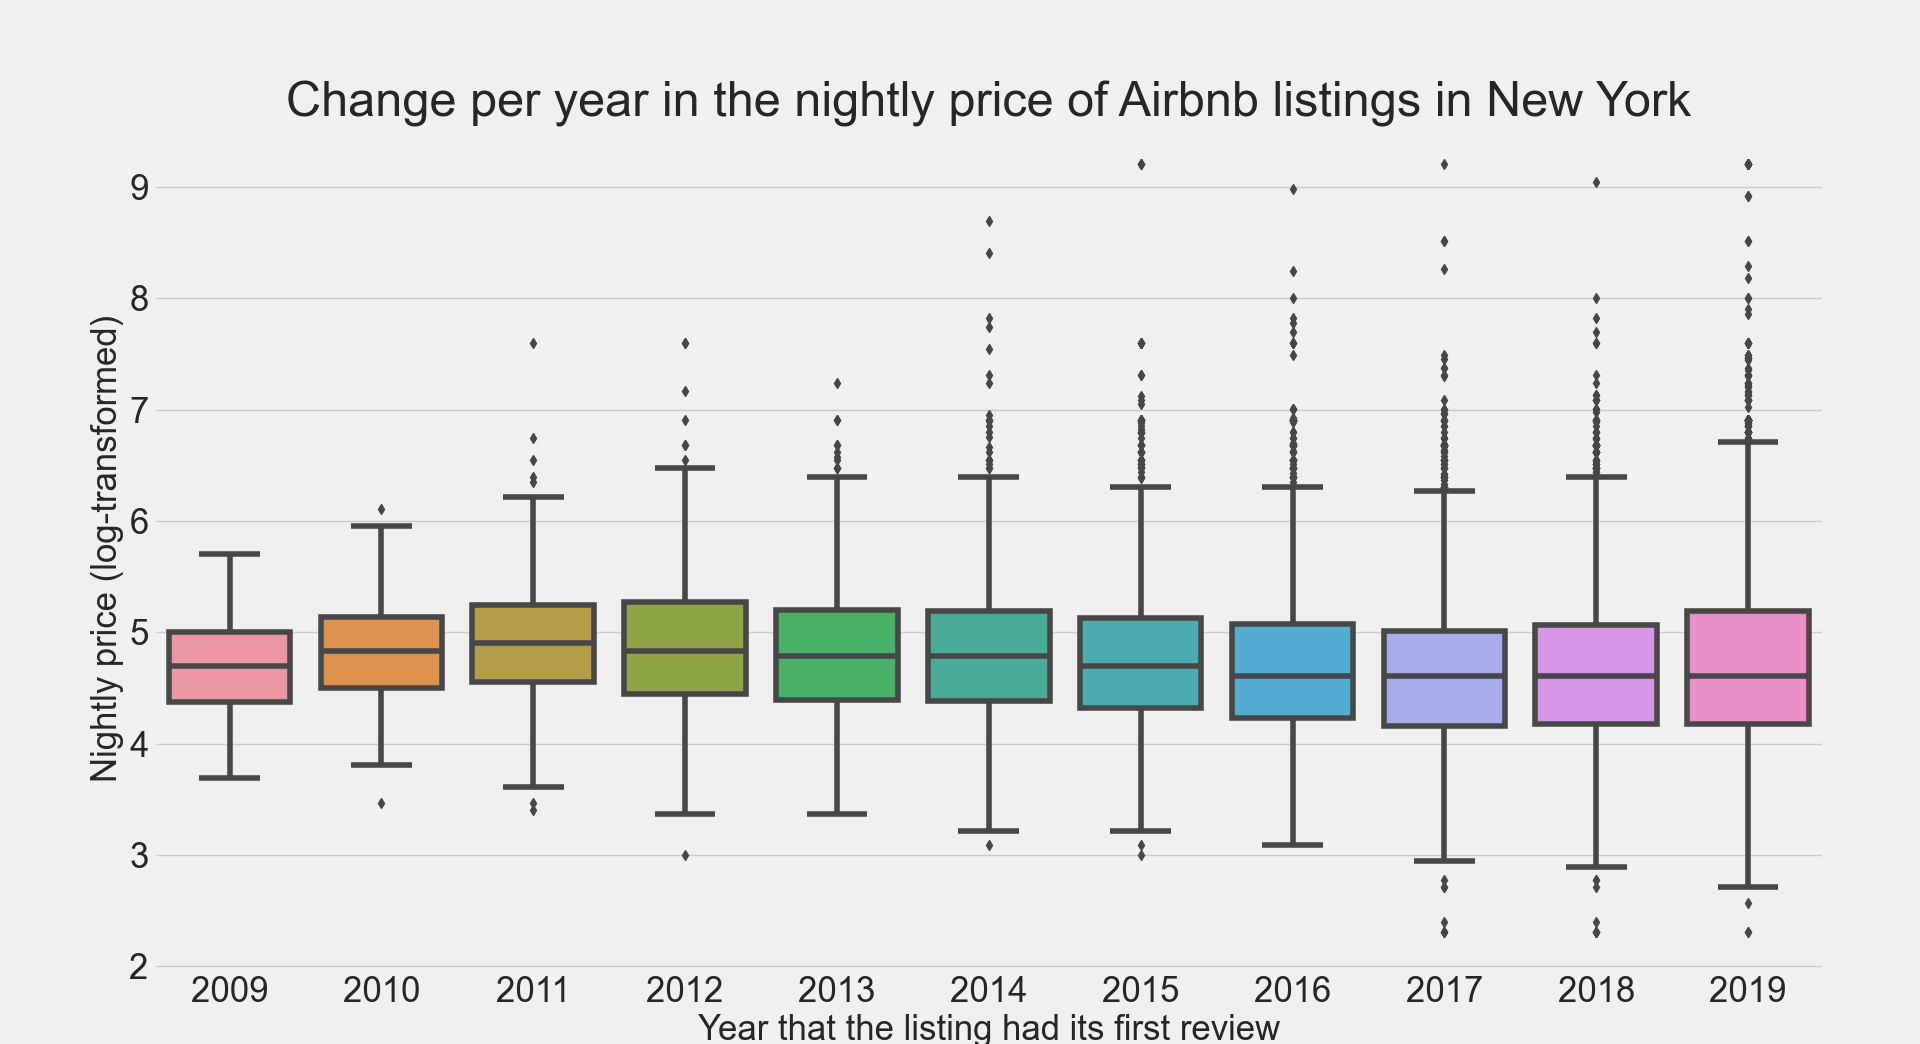
\includegraphics[width=\textwidth]{price-trend.png}
    \caption{Change per year in the nightly price of Airbnb listings in New York}
    \label{fig:prices-change-by-years}
\end{figure}


\section{Modelling}

\subsection{Training and Test Sets}
\label{sec:train_test_split}

The train-test split procedure is used to estimate machine learning algorithms'
performance when making predictions on data not used to train the model.  We
randomly split the dataset into 80\% and 20\% of listings for training and test
sets, respectively. The training set is used to fit the model, and the test
set is used to evaluate the fit machine learning model. The objective is to
estimate the machine learning model's performance on new data: data not used to
train the model.

The scikit-learn library provides an implementation of the train-test-split
procedure via the \texttt{train\_test\_split()} function.

\subsection{Findings}
\label{sec:findings}

A summary of of results is reported in Table ~\ref{tab:results}

\begin{table}[!htbp]
  \centering
  \caption{Results}
  \label{tab:results}
  \begin{tabular}{lllll}
    \hline
    ML Algorithm & Training MSE & Test MSE & Training $R^2$ & Test $R^2$ \\
    \hline
    Linear Regresion & 0.1291 &  8.5E21 &  0.7019 & -1.9E22 \\
    Ridge Regression  & 0.1291 & 0.138 & 0.7019 &  0.6857 \\
    Lasso Regression & 0.1351 & 0.1441 & 0.688 & 0.6718 \\
    XGboost &  0.0798 & 0.1173 & 0.8157 &  0.7328 \\
  \end{tabular}
\end{table}


As expected in ~\ref{linear-regression} incorporating such a large number
of features (309) makes the linear regression model overfit the data. As
shown in Table ~\ref{tab:results}, while training MSE of the linear regression
model is quite good, the model performs poorly on the test set both in terms of
in terms of $MSE$ and $R^2$.

By performing k-fold cross-validation with ten folds, we can find the tuning
parameter's value that results in the smallest cross-validation error is 115.
The test's MSE is associated with this value of  is 0.138.  The result
represents a considerable improvement of ridge regression over the test MSE we
got using least square regression.


Using cross-validation , we find the optimized penalty value $\lambda$ for lasso
is 0.005.  The associated test MSE is 0.1441, which is slightly higher than the
test set MSE of the ridge regression.  Recall from that the advantage of using
lasso regression over ridge regression is that lasso performs feature selection.
Lasso picked 153 variables while eliminated the other 125 features.


As shown by the Table ~\ref{tab:results}, XGboost consistently outperforms these
competing approaches in both mean squared error and R-squared.  With this model,
the features explain approximately 73\% of the target variable's variance and
have smaller MSE than the other regression model.

\begin{table}[!htbp]
  \centering
  \caption{XGBoost Top 20 Feature Weights}
  \label{tab:xgb-weights}
  \begin{tabular}{lr}
    \toprule
    {} &    weight \\
    \midrule
    room\_type\_Entire home/apt        &  0.336396 \\
    bathrooms                        &  0.032001 \\
    neighbourhood\_Midtown            &  0.025008 \\
    neighbourhood\_Hell's Kitchen     &  0.018545 \\
    neighbourhood\_East Village       &  0.015763 \\
    property\_type\_Other              &  0.015168 \\
    neighbourhood\_Bedford-Stuyvesant &  0.014314 \\
    neighbourhood\_West Village       &  0.014031 \\
    neighbourhood\_Chelsea            &  0.013612 \\
    neighbourhood\_Lower East Side    &  0.011874 \\
    neighbourhood\_Bushwick           &  0.011854 \\
    neighbourhood\_Upper West Side    &  0.011682 \\
    neighbourhood\_Washington Heights &  0.011659 \\
    neighbourhood\_SoHo               &  0.011582 \\
    room\_type\_Shared room            &  0.011304 \\
    neighbourhood\_Greenwich Village  &  0.010347 \\
    room\_type\_Hotel room             &  0.009697 \\
    neighbourhood\_Theater District   &  0.008575 \\
    neighbourhood\_Williamsburg       &  0.008490 \\
    neighbourhood\_Crown Heights      &  0.007979 \\
  \bottomrule
  \end{tabular}
\end{table}

Another important finding from \ref{tab:xgb-weights} was the role of location
features play in predicting price. In particular, location features located in
Manhattan and Brooklyn borough are in the top 20 important variables to predict
the price. This is consistent with what we observed in \ref{eda:neighbourhood}.




\clearpage
\chapter{Conclusion and Future Works}
\label{c:conclusion}
This study's primary purpose was to evaluate the predictive performance of
various machine learning models to real data on Airbnb listings in the city of
New York.  The methods used in this study consisted of simple and multiple
linear regression, ridge regression, lasso regression, and XGBoost. The models
were compared and assessed using mean square error and coefficient of
determination criteria.

The research has shown that gradient boosting with all features (XGBoost) performs
the best among all models. Ridge regression has the second-best performance.
While Lasso's performance is not as good as Ridge Regression and XGBoost, Lasso
performs feature selection. With Lasso, we were able to find a sparse model,
which includes only relevant variables.
Linear Regression performs the worst proved that the abundance of features leads
to high variance and weak performance (overfitting).

The second aim of this study was to identify which characteristics of an Airbnb
listing were most important in predicting the price. We found that the most
critical feature is whether the type of listing is an entire home or not. The
second most important feature is the number of bathrooms. Also, location
features play an essential role in predicting price. These findings help
develop a reliable price prediction model to aid the Airbnb hosts in maximizing
their earnings.

In future work, we would like to:
\begin{enumerate}
  \item Experiment with the data with Neural Network.
  \item Find a way to include listing's photo quality as a predictor.
  \item Incorporate customer reviews feature through sentiment analysis.
\end{enumerate}




\clearpage
	\setcounter{chapter}{1}
	\fancyhf{}
	\rhead{\thepage}
	\lhead{\textbf{Appendices}}
\phantomsection
\addcontentsline{toc}{chapter}{Appendices}
\renewcommand{\thechapter}{\Alph{chapter}}
\pagenumbering{roman}

\appendix
\section*{Appendices}
\label{chap_appendices}
\section{Tables}
\begin{table}[H]
    \centering
    \caption{Summary Statistics}
    \label{tab:descriptive-statistic}
{\small

\begin{tabular}{lrr}
\toprule
{} &      mean &          std \\
\midrule
host\_is\_superhost      &     0.234 &        0.424 \\
host\_listings\_count    &     7.775 &       54.391 \\
host\_identity\_verified &     0.486 &        0.500 \\
accommodates           &     2.906 &        1.911 \\
bathrooms              &     1.140 &        0.421 \\
bedrooms               &     1.183 &        0.750 \\
beds                   &     1.570 &        1.156 \\
price                  &   138.085 &      118.185 \\
security\_deposit       &   172.822 &      406.817 \\
cleaning\_fee           &    54.161 &       54.671 \\
guests\_included        &     1.584 &        1.210 \\
extra\_people           &    15.986 &       25.143 \\
minimum\_nights         &     6.151 &       19.285 \\
maximum\_nights         & 55397.541 & 10750846.675 \\
availability\_90        &    32.857 &       33.807 \\
number\_of\_reviews      &    31.090 &       51.014 \\
instant\_bookable       &     0.382 &        0.486 \\
host\_days\_active       &  1654.499 &      885.855 \\
air\_conditioning       &     0.867 &        0.339 \\
bed\_linen              &     0.349 &        0.477 \\
tv                     &     0.685 &        0.465 \\
coffee\_machine         &     0.339 &        0.473 \\
cooking\_basics         &     0.370 &        0.483 \\
white\_goods            &     0.447 &        0.497 \\
elevator               &     0.250 &        0.433 \\
child\_friendly         &     0.280 &        0.449 \\
parking                &     0.469 &        0.499 \\
host\_greeting          &     0.171 &        0.377 \\
internet               &     0.984 &        0.126 \\
long\_term\_stays        &     0.218 &        0.413 \\
pets\_allowed           &     0.165 &        0.371 \\
private\_entrance       &     0.210 &        0.407 \\
self\_check\_in          &     0.260 &        0.438 \\
\bottomrule
\end{tabular}
}
\end{table}

\begin{flushleft}
\begin{table}[H]
    \small
    \caption{The variable list}
    \label{tab:variable-list}
    \begin{tabular}{ll}
    \hline
    Variables & Definition \\
    \hline
    experience\_offerd & recommended category of travel type, e.g. business \\
    host\_since & date that the host first joined Airbnb \\
    host\_response\_time & average amount of time the host takes to reply to messages \\
    host\_response\_rate & proportion of messages that the host replies to \\
    host\_is\_superhost &
    \begin{tabular}{@{}l@{}l@{}} whether or not the host is a superhost, which is a
        mark of \\ mark of quality for the top-rated and most experienced hosts,
        \\ and can increase your search ranking on Airbnb \end{tabular} \\
    host\_listings\_count & how many listings the host has in total \\
    host\_identity\_verified & whether or not the host has been verified with id \\
    neighbourhood\_cleansed & NewYork  borough the property is in \\
    property\_type & type of property, e.g. house or flat \\
    room\_type & type of listing, e.g. entire home, private room or shared room \\
    accommodates & how many people the property accommodates \\
    bathrooms & number of bathrooms \\
    bedrooms & number of bedrooms \\
    beds & number of beds \\
    bed\_type & type of bed, e.g. real bed or sofa-bed \\
    amenities & list of amenities \\
    price & nightly advertised price (the target variable) \\
    security\_deposit & the amount required as a security deposit \\
    cleaning\_fee & the amount of the cleaning fee (a fixed amount paid per booking)
    \\
    guests\_included & the number of guests included in the booking fee \\
    extra\_people & the price per additional guest above the guests\_included price
    \\
    minimum\_nights & the minimum length of stay \\
    maximum\_nights & the maximum length of stay \\
    calendar\_updated & when the host last updated the calendar \\
    availability\_30 & how many nights are available to be booked in the next 30
    days \\
    availability\_60 & how many nights are available to be booked in the next 60
    days \\
    availability\_90 & how many nights are available to be booked in the next 90
    days \\
    availability\_365 & how many nights are available to be booked in the next
    365 days \\
    number\_of\_reviews & the number of reviews left for the property \\
    number\_of\_reviews\_ltm & the number of reviews left for the property in the
    last twelve months \\
    first\_review & the date of the first review \\
    last\_review & the date of the most recent review \\
    review\_scores\_rating & guests can score properties overall from 1 to 5 stars
    \\
    review\_scores\_accuracy &  accuracy score of a property's description from 1 to 5 stars \\
    review\_scores\_cleanliness & guests can score a property's cleanliness from 1
    to 5 stars \\
    review\_scores\_checkin & guests can score their check-in from 1 to 5 stars \\
    review\_scores\_communication & guests can score a host's communication from 1
    to 5 stars \\
    review\_scores\_location & guests can score a property's location from 1 to 5
    stars \\
    review\_scores\_value & guests can score a booking's value for money from 1 to 5
    stars \\
    instant\_bookable &
    \begin{tabular}{@{}l@{}l@{}}
            whether or not the property can be instant booked (i.e.
            booked \\ straight away, without having to message the host first
            and wait to \\ be accepted)
        \end{tabular} \\
    cancellation\_policy & the type of cancellation policy, e.g. strict or moderate \\
    reviews\_per\_month & average number of reviews left by guest each month \\
\end{tabular}
\end{table}
\end{flushleft}


\section{Figures}

\begin{figure}[H] \centering
    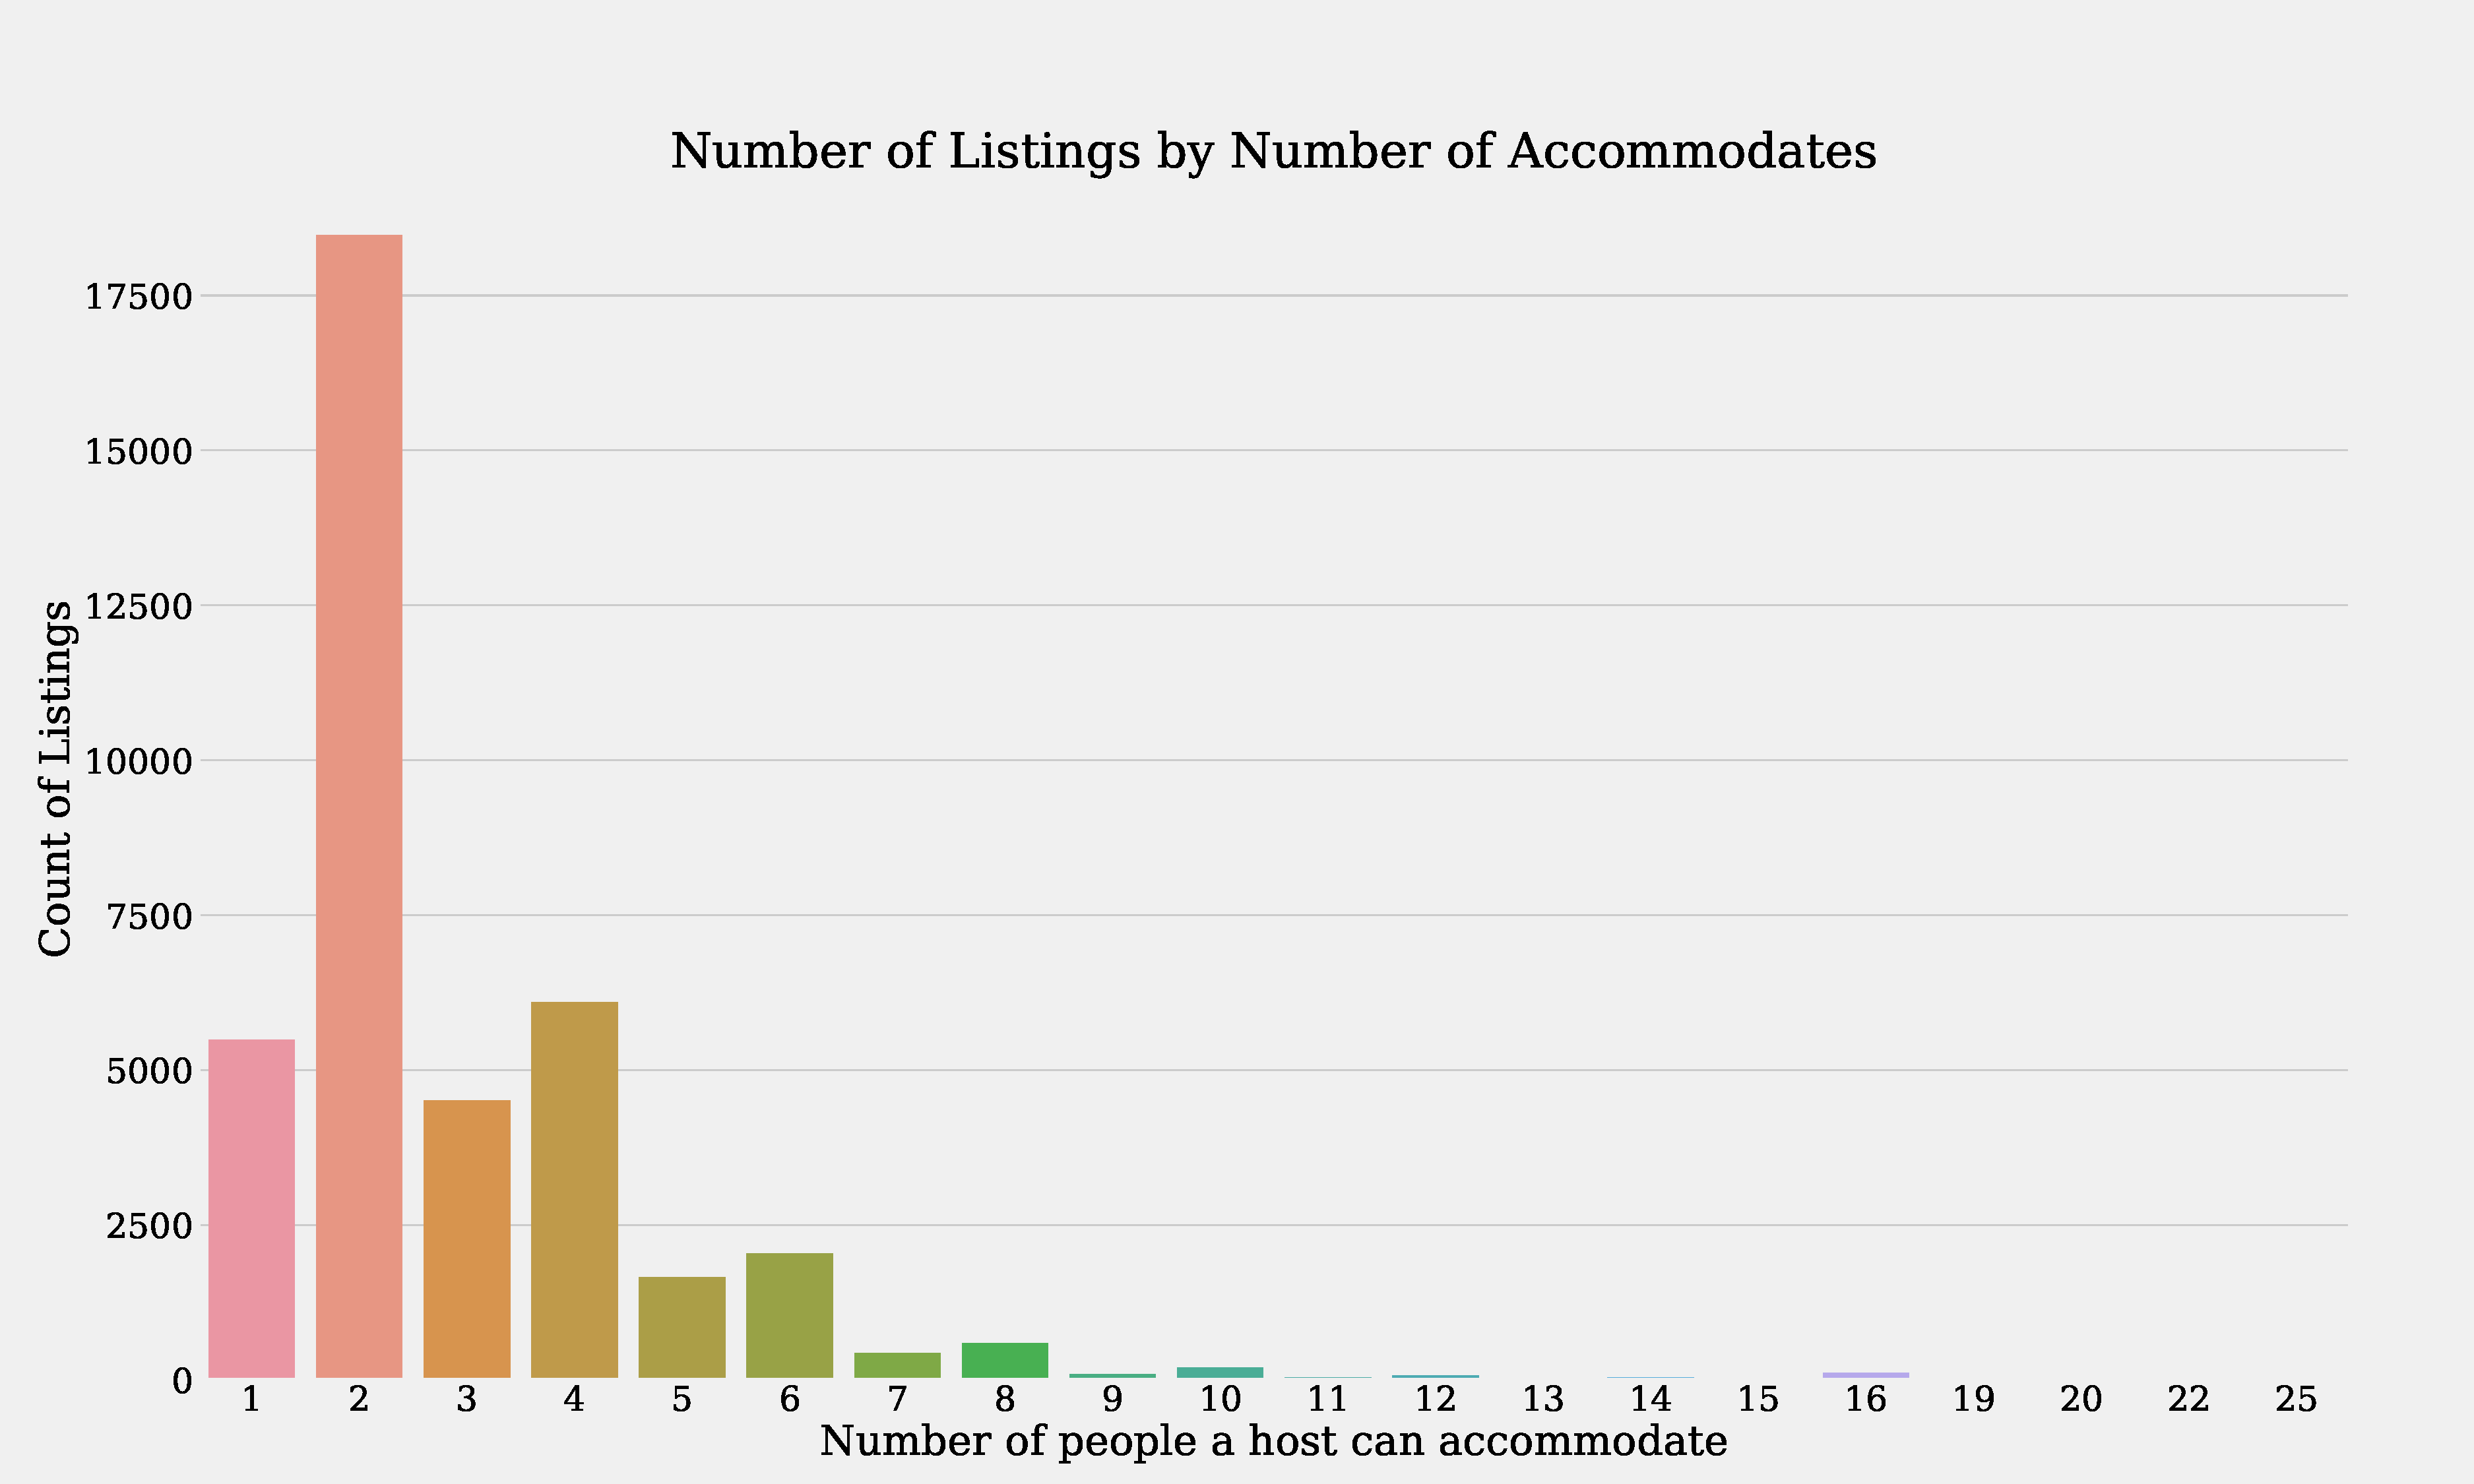
\includegraphics[width=\textwidth]{accommodates-countplot.pdf}
    \caption{Number of Listings by Accomodates}
    \label{fig:accommodates-countplot}
\end{figure}

\begin{figure}[H] \centering
    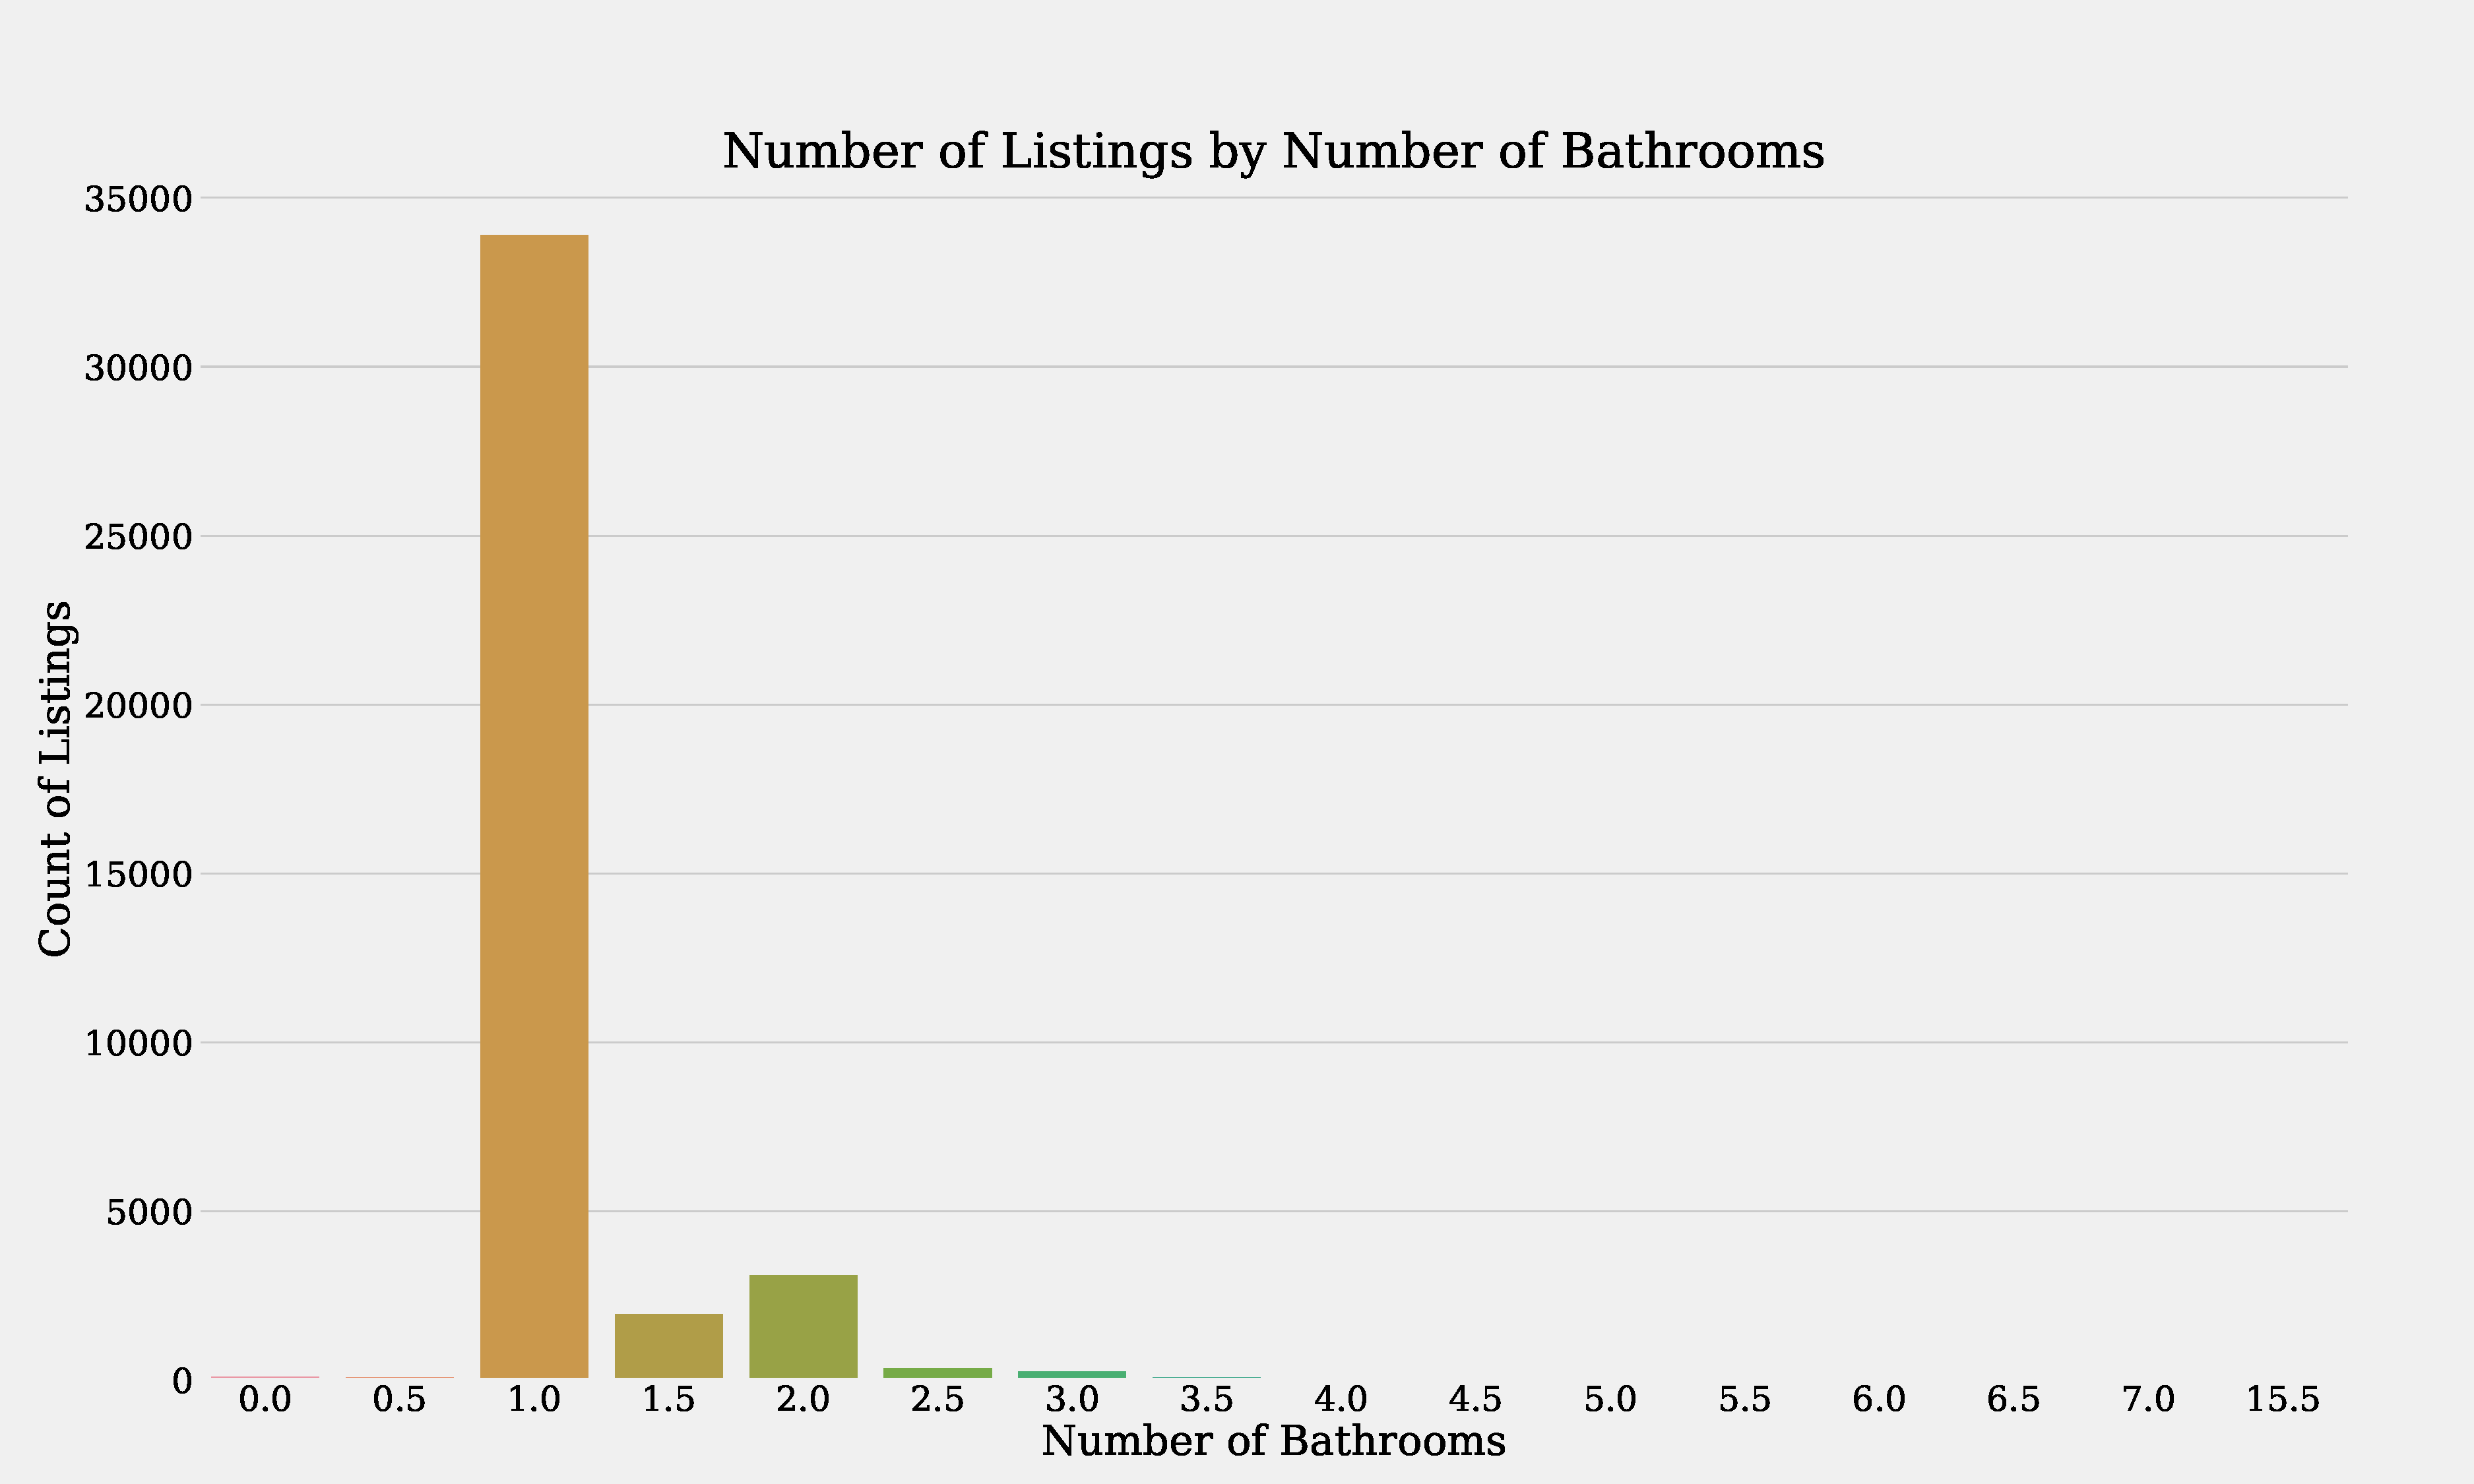
\includegraphics[width=\textwidth]{bathrooms-countplot.pdf}
    \caption{Number of Listings by Number of Bathrooms }
    \label{fig:bathrooms-countplot}
\end{figure}

\begin{figure}[H] \centering
    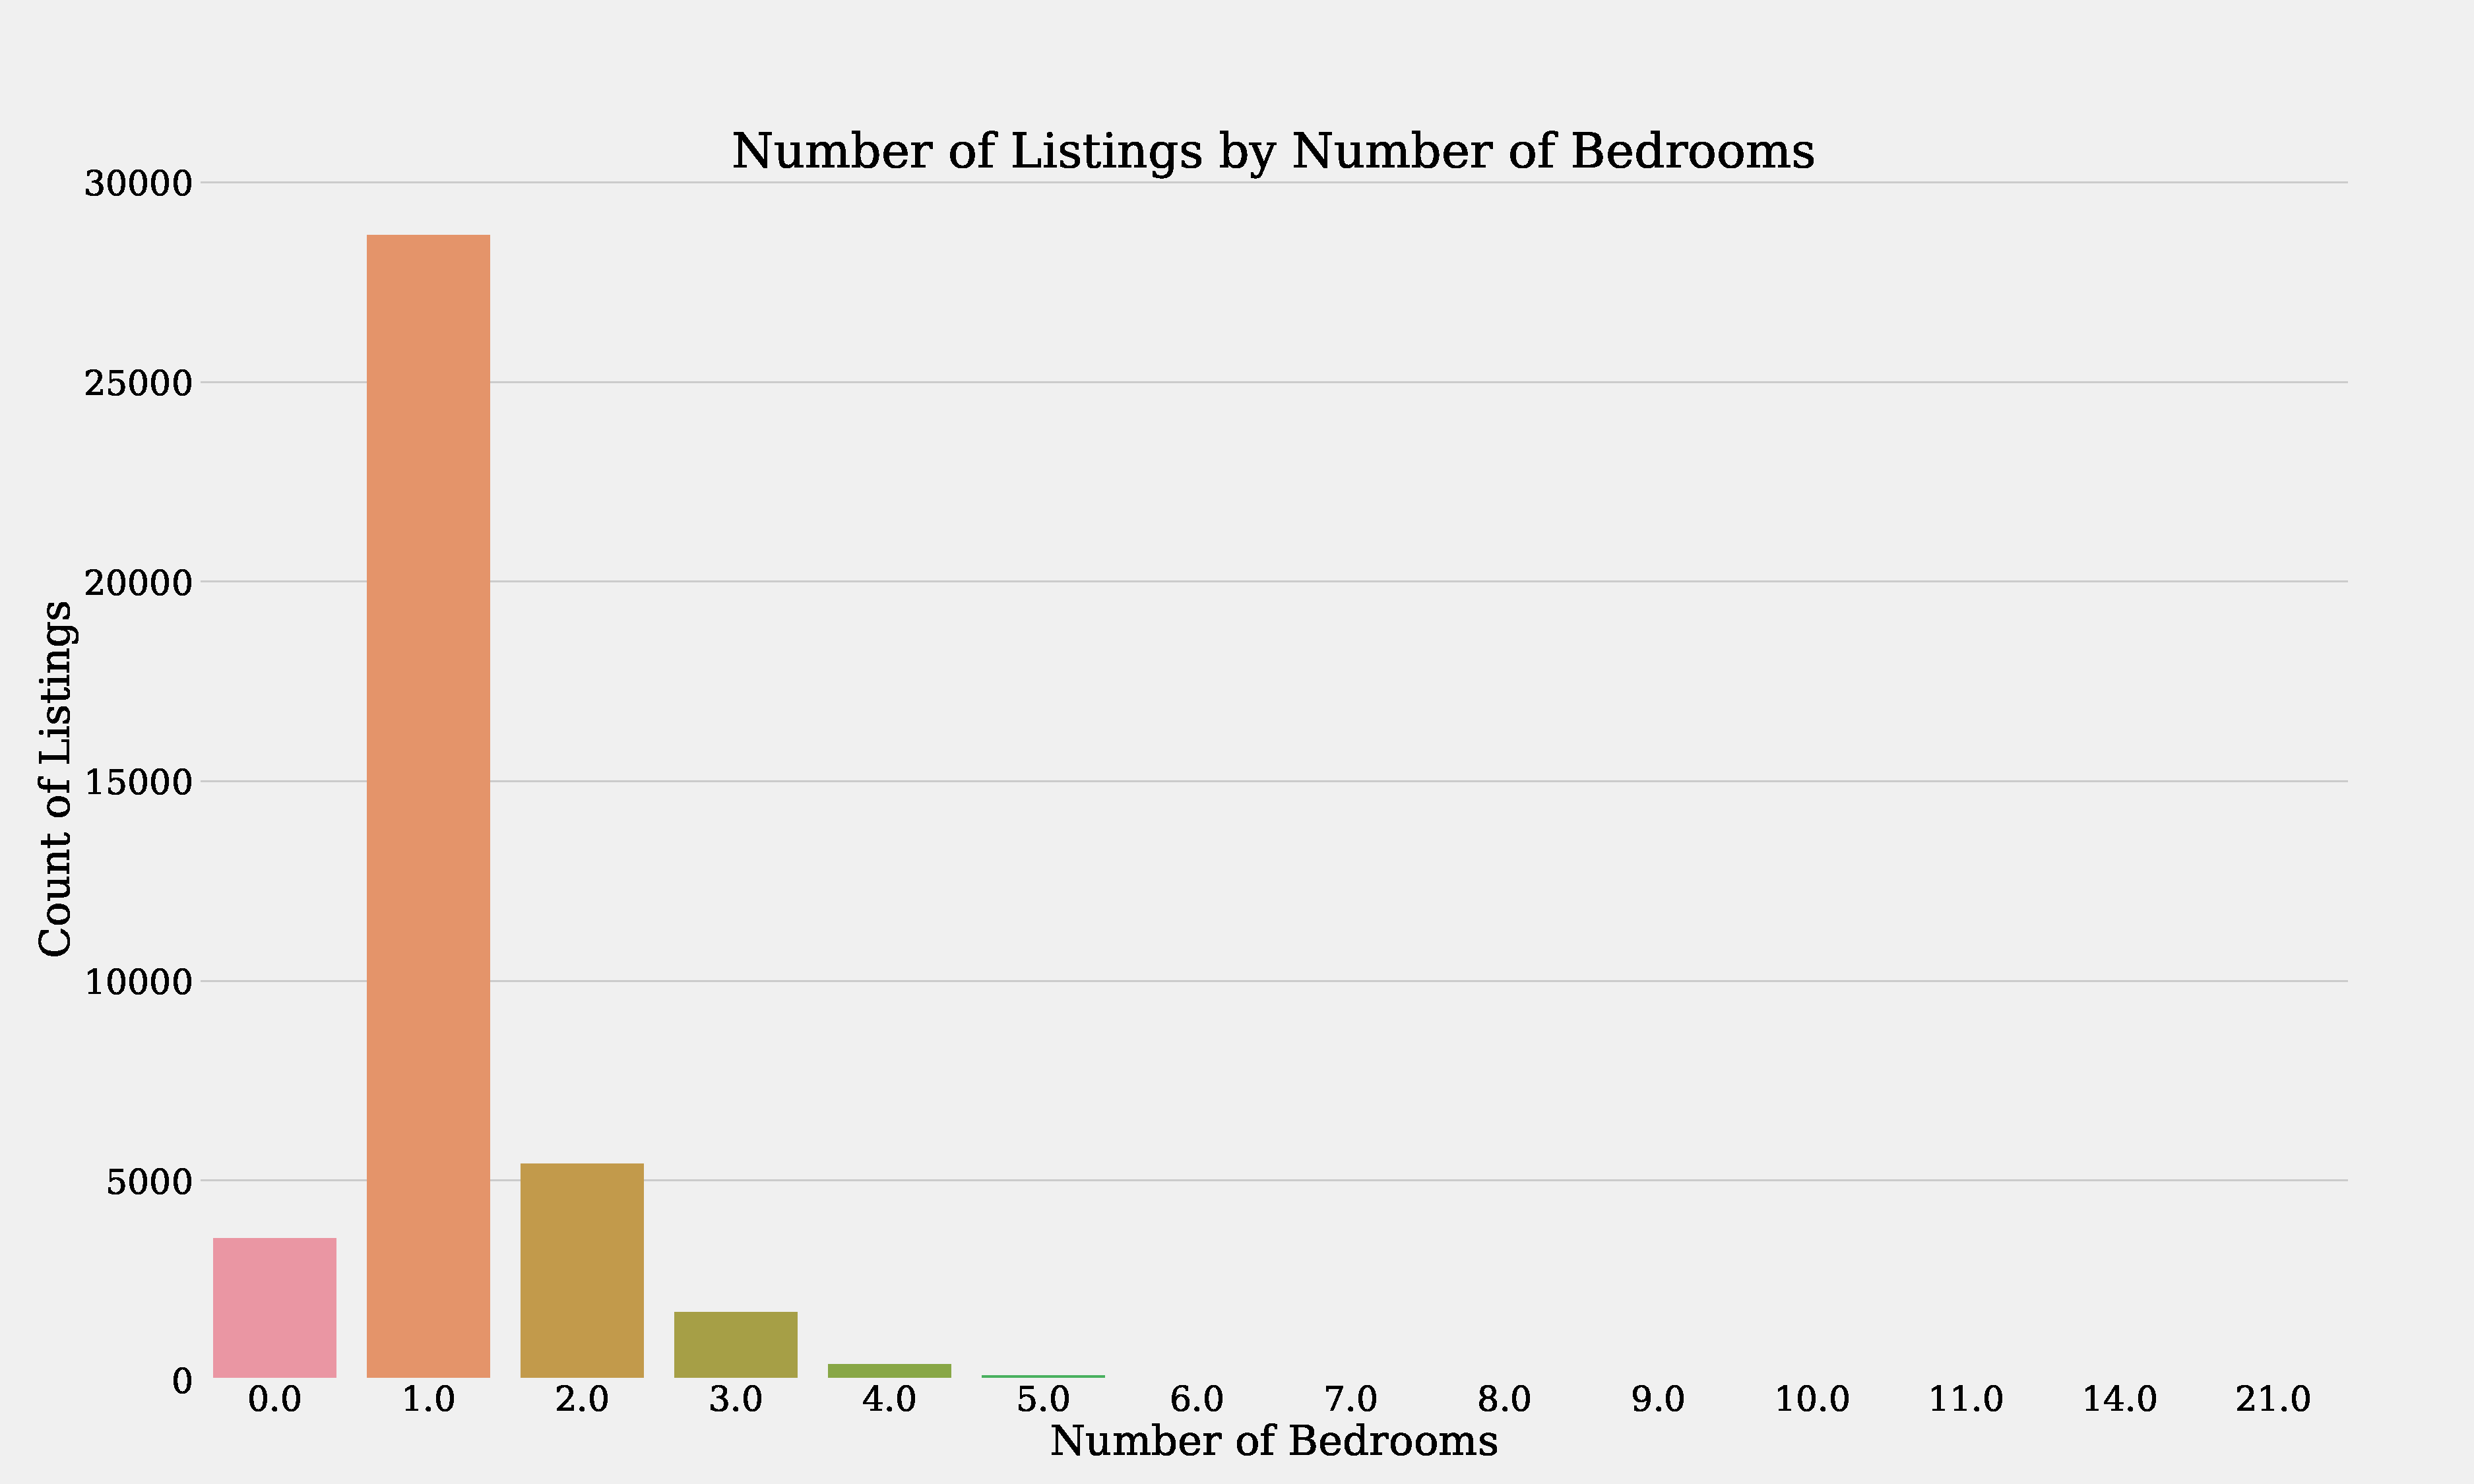
\includegraphics[width=\textwidth]{bedrooms-countplot.pdf}
    \caption{Number of Listings by Number of Bedrooms }
    \label{fig:bedrooms-countplot}
\end{figure}

\begin{figure}[H] \centering
    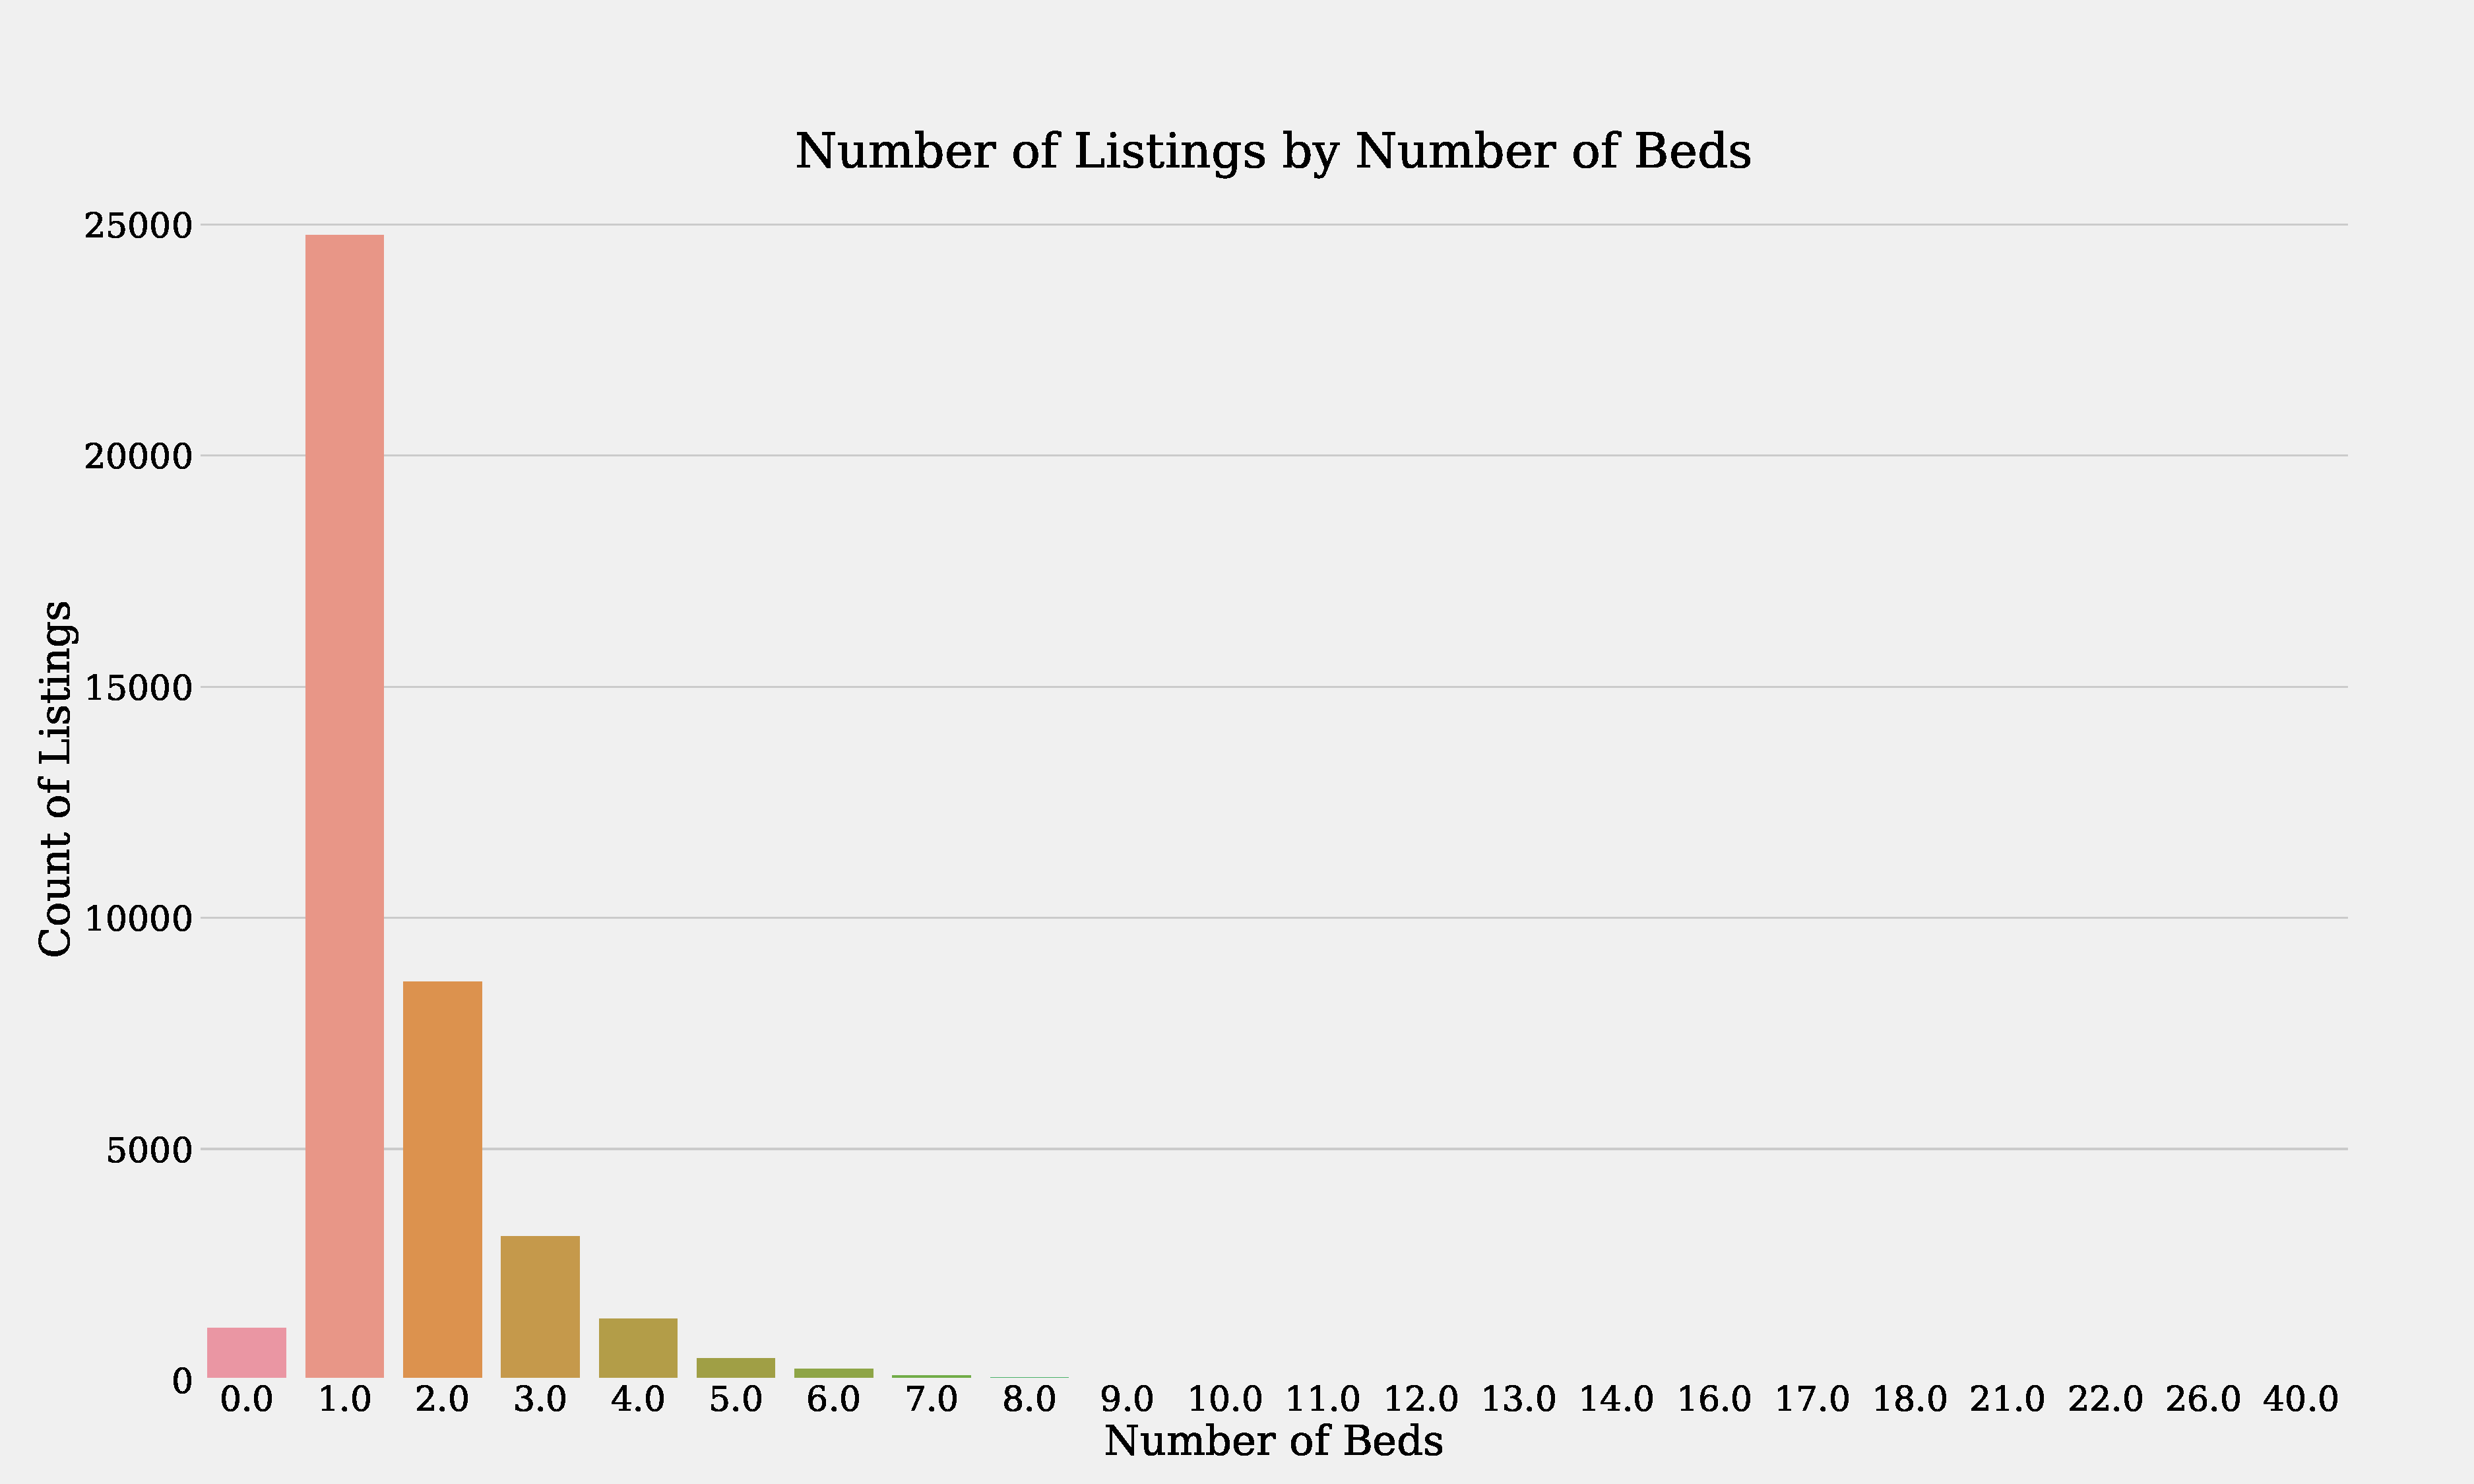
\includegraphics[width=\textwidth]{beds-countplot.pdf}
    \caption{Number of Listings by Number of Beds }
    \label{fig:beds-countplot}
\end{figure}

% ------------------------------
% median price by accommodates, bathrooms, bedrooms, beds
\begin{figure}[H] \centering
    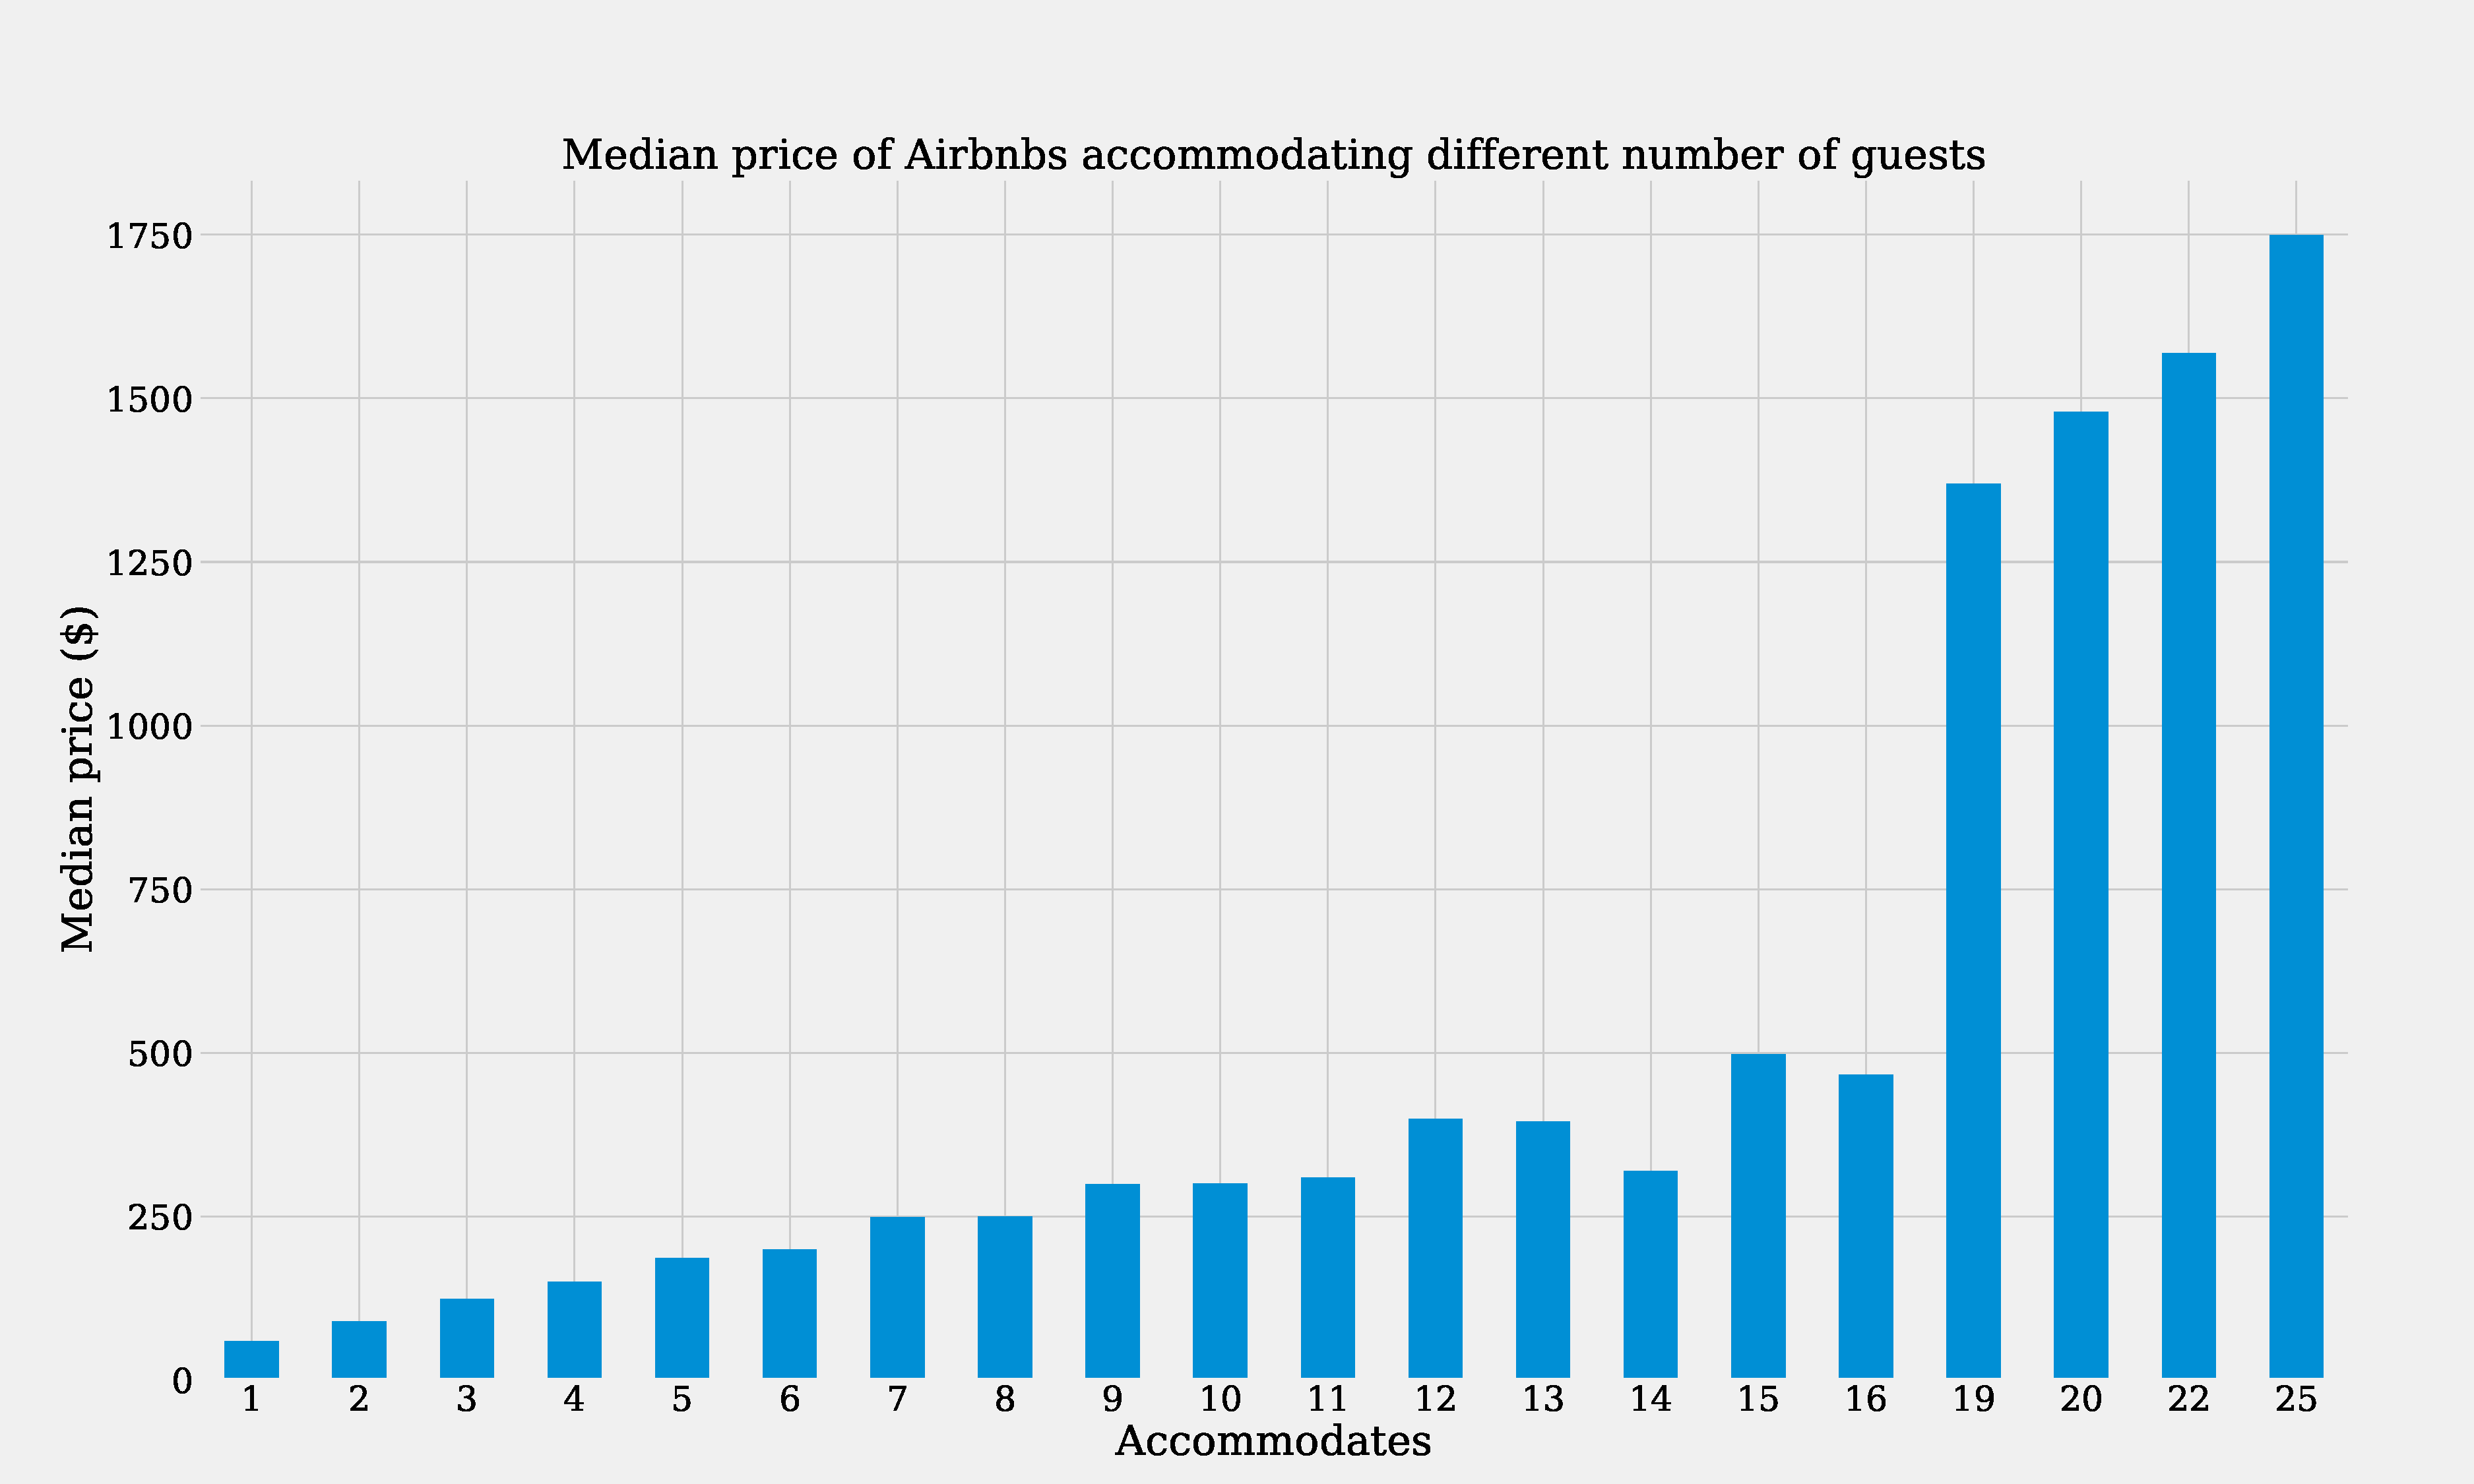
\includegraphics[width=\textwidth]{median-price-by-accommodates.pdf}
    \caption{Median Price By Accommodates}
    \label{fig:median-price-by-accommodates}
\end{figure}

\begin{figure}[H] \centering
    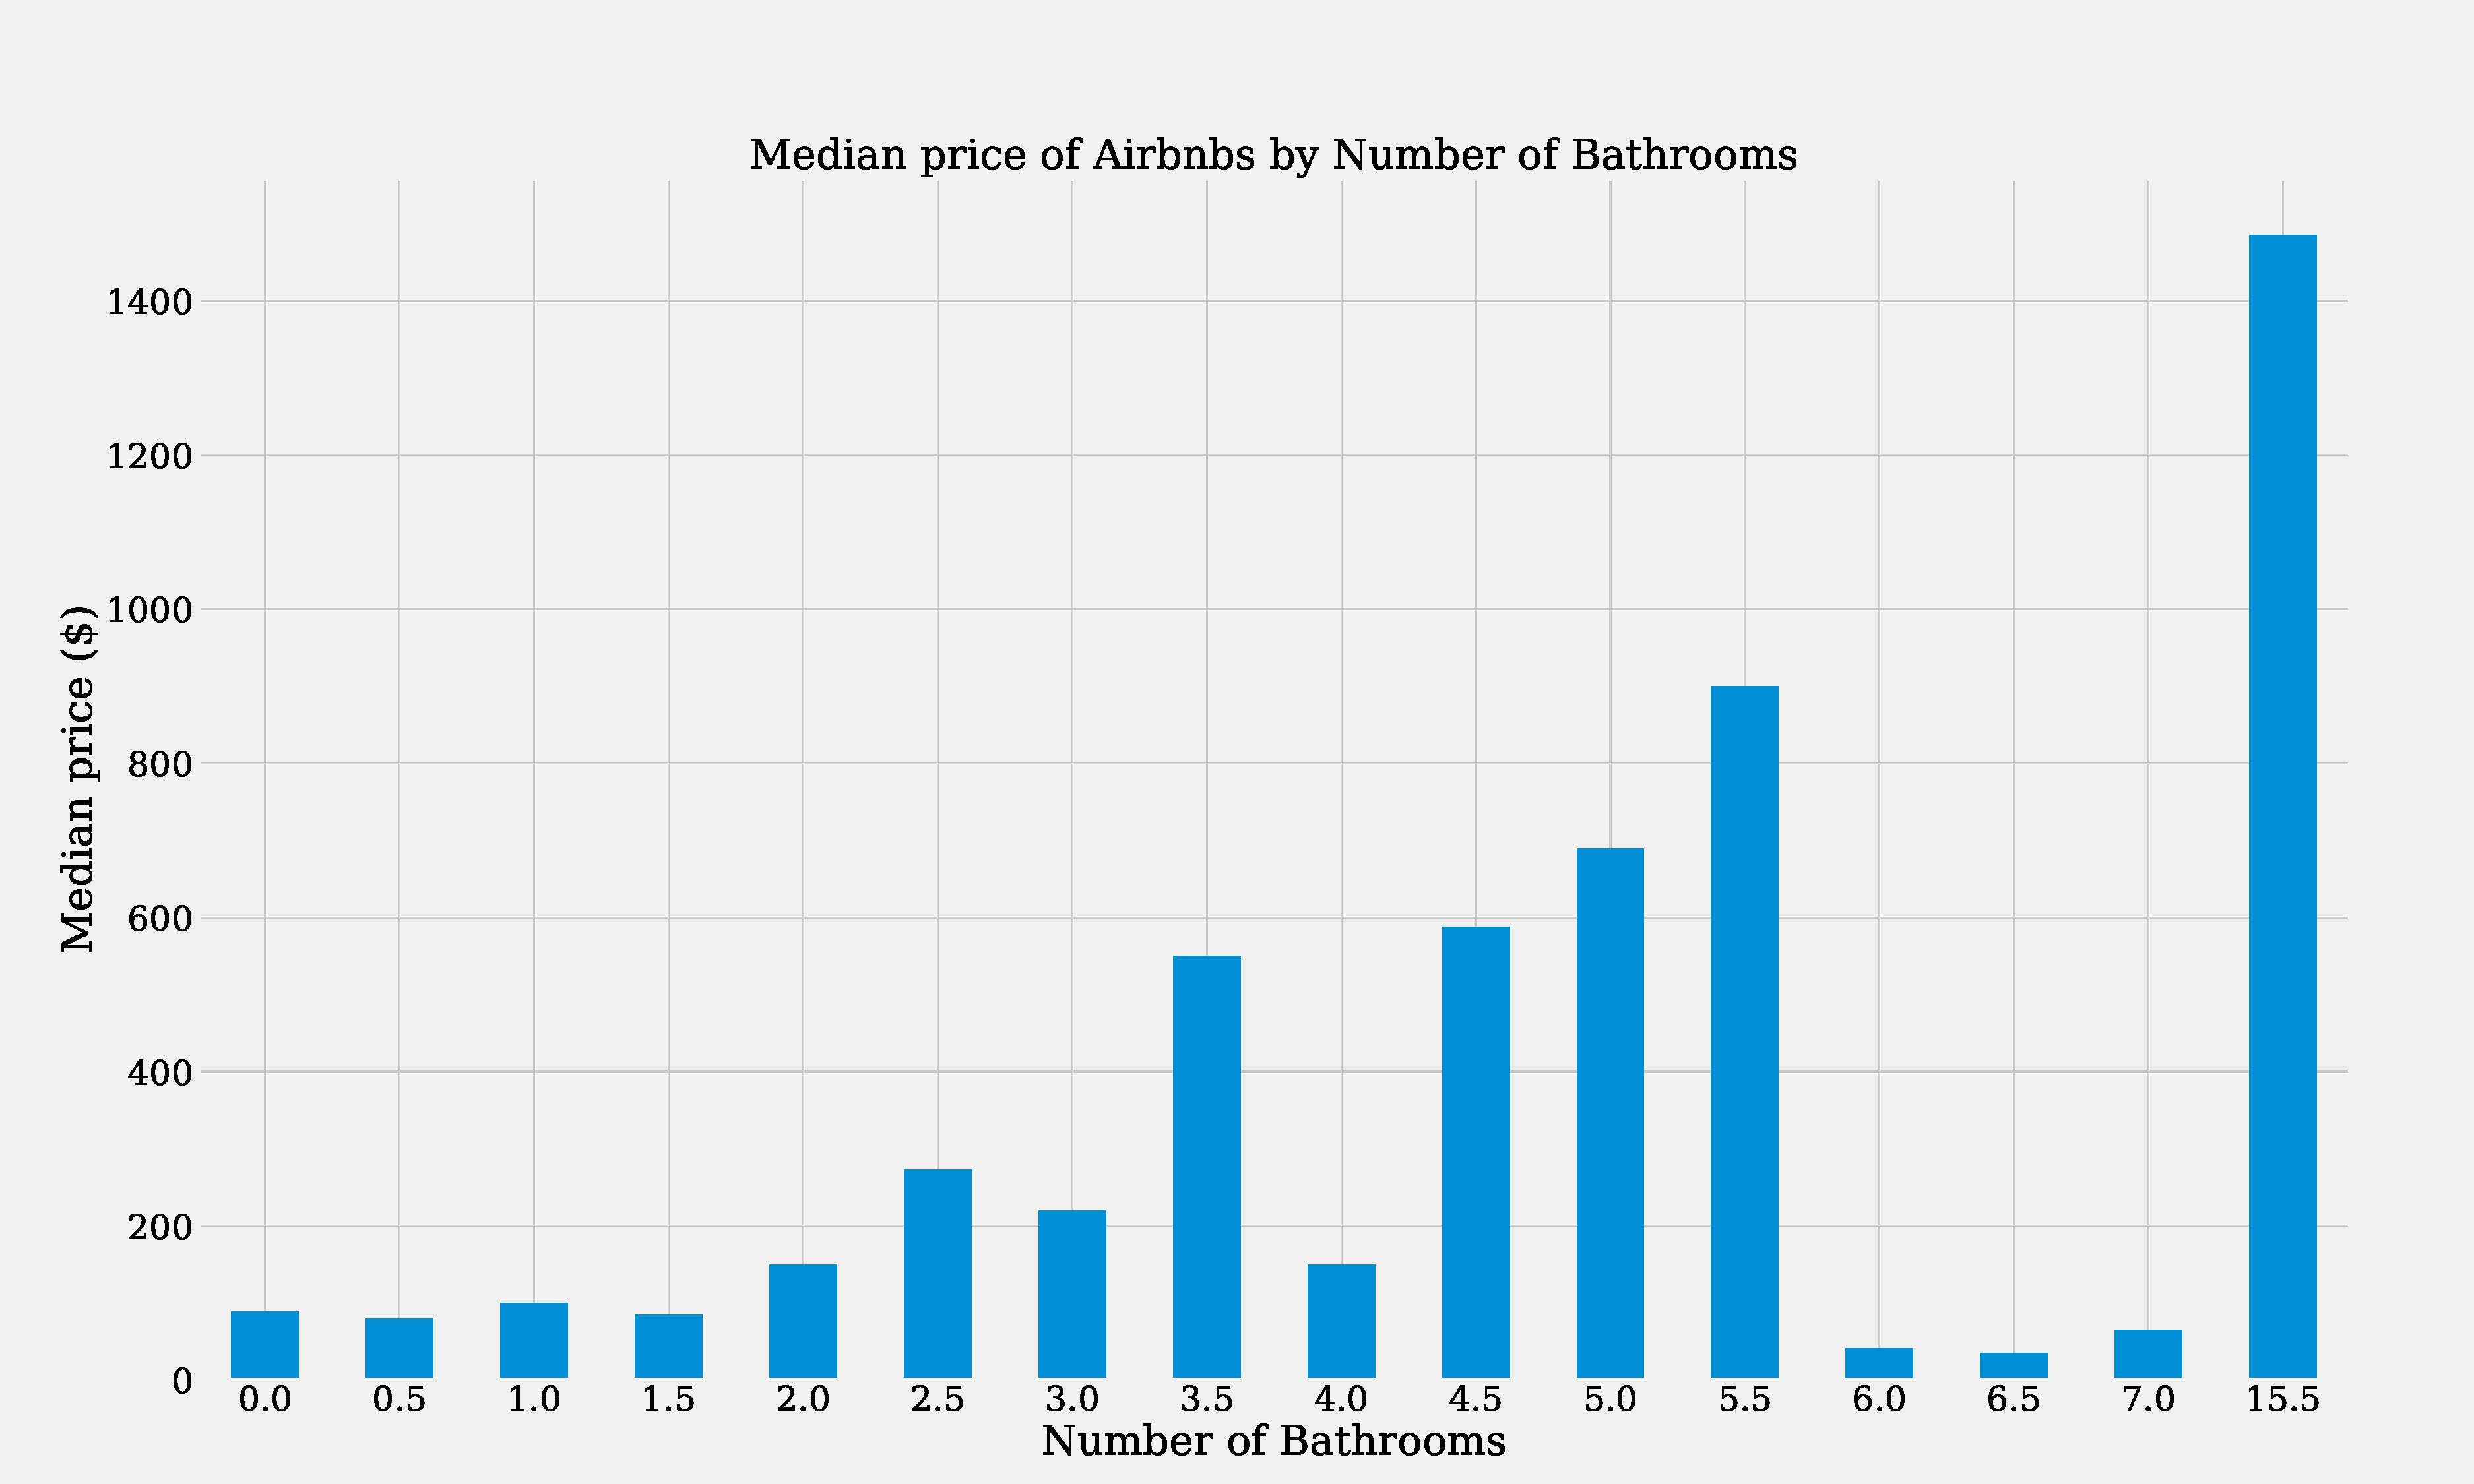
\includegraphics[width=\textwidth]{median-price-by-bathrooms.pdf}
    \caption{Median Price By  Number of Bathrooms }
    \label{fig:median-price-by-bathrooms}
\end{figure}

\begin{figure}[H] \centering
    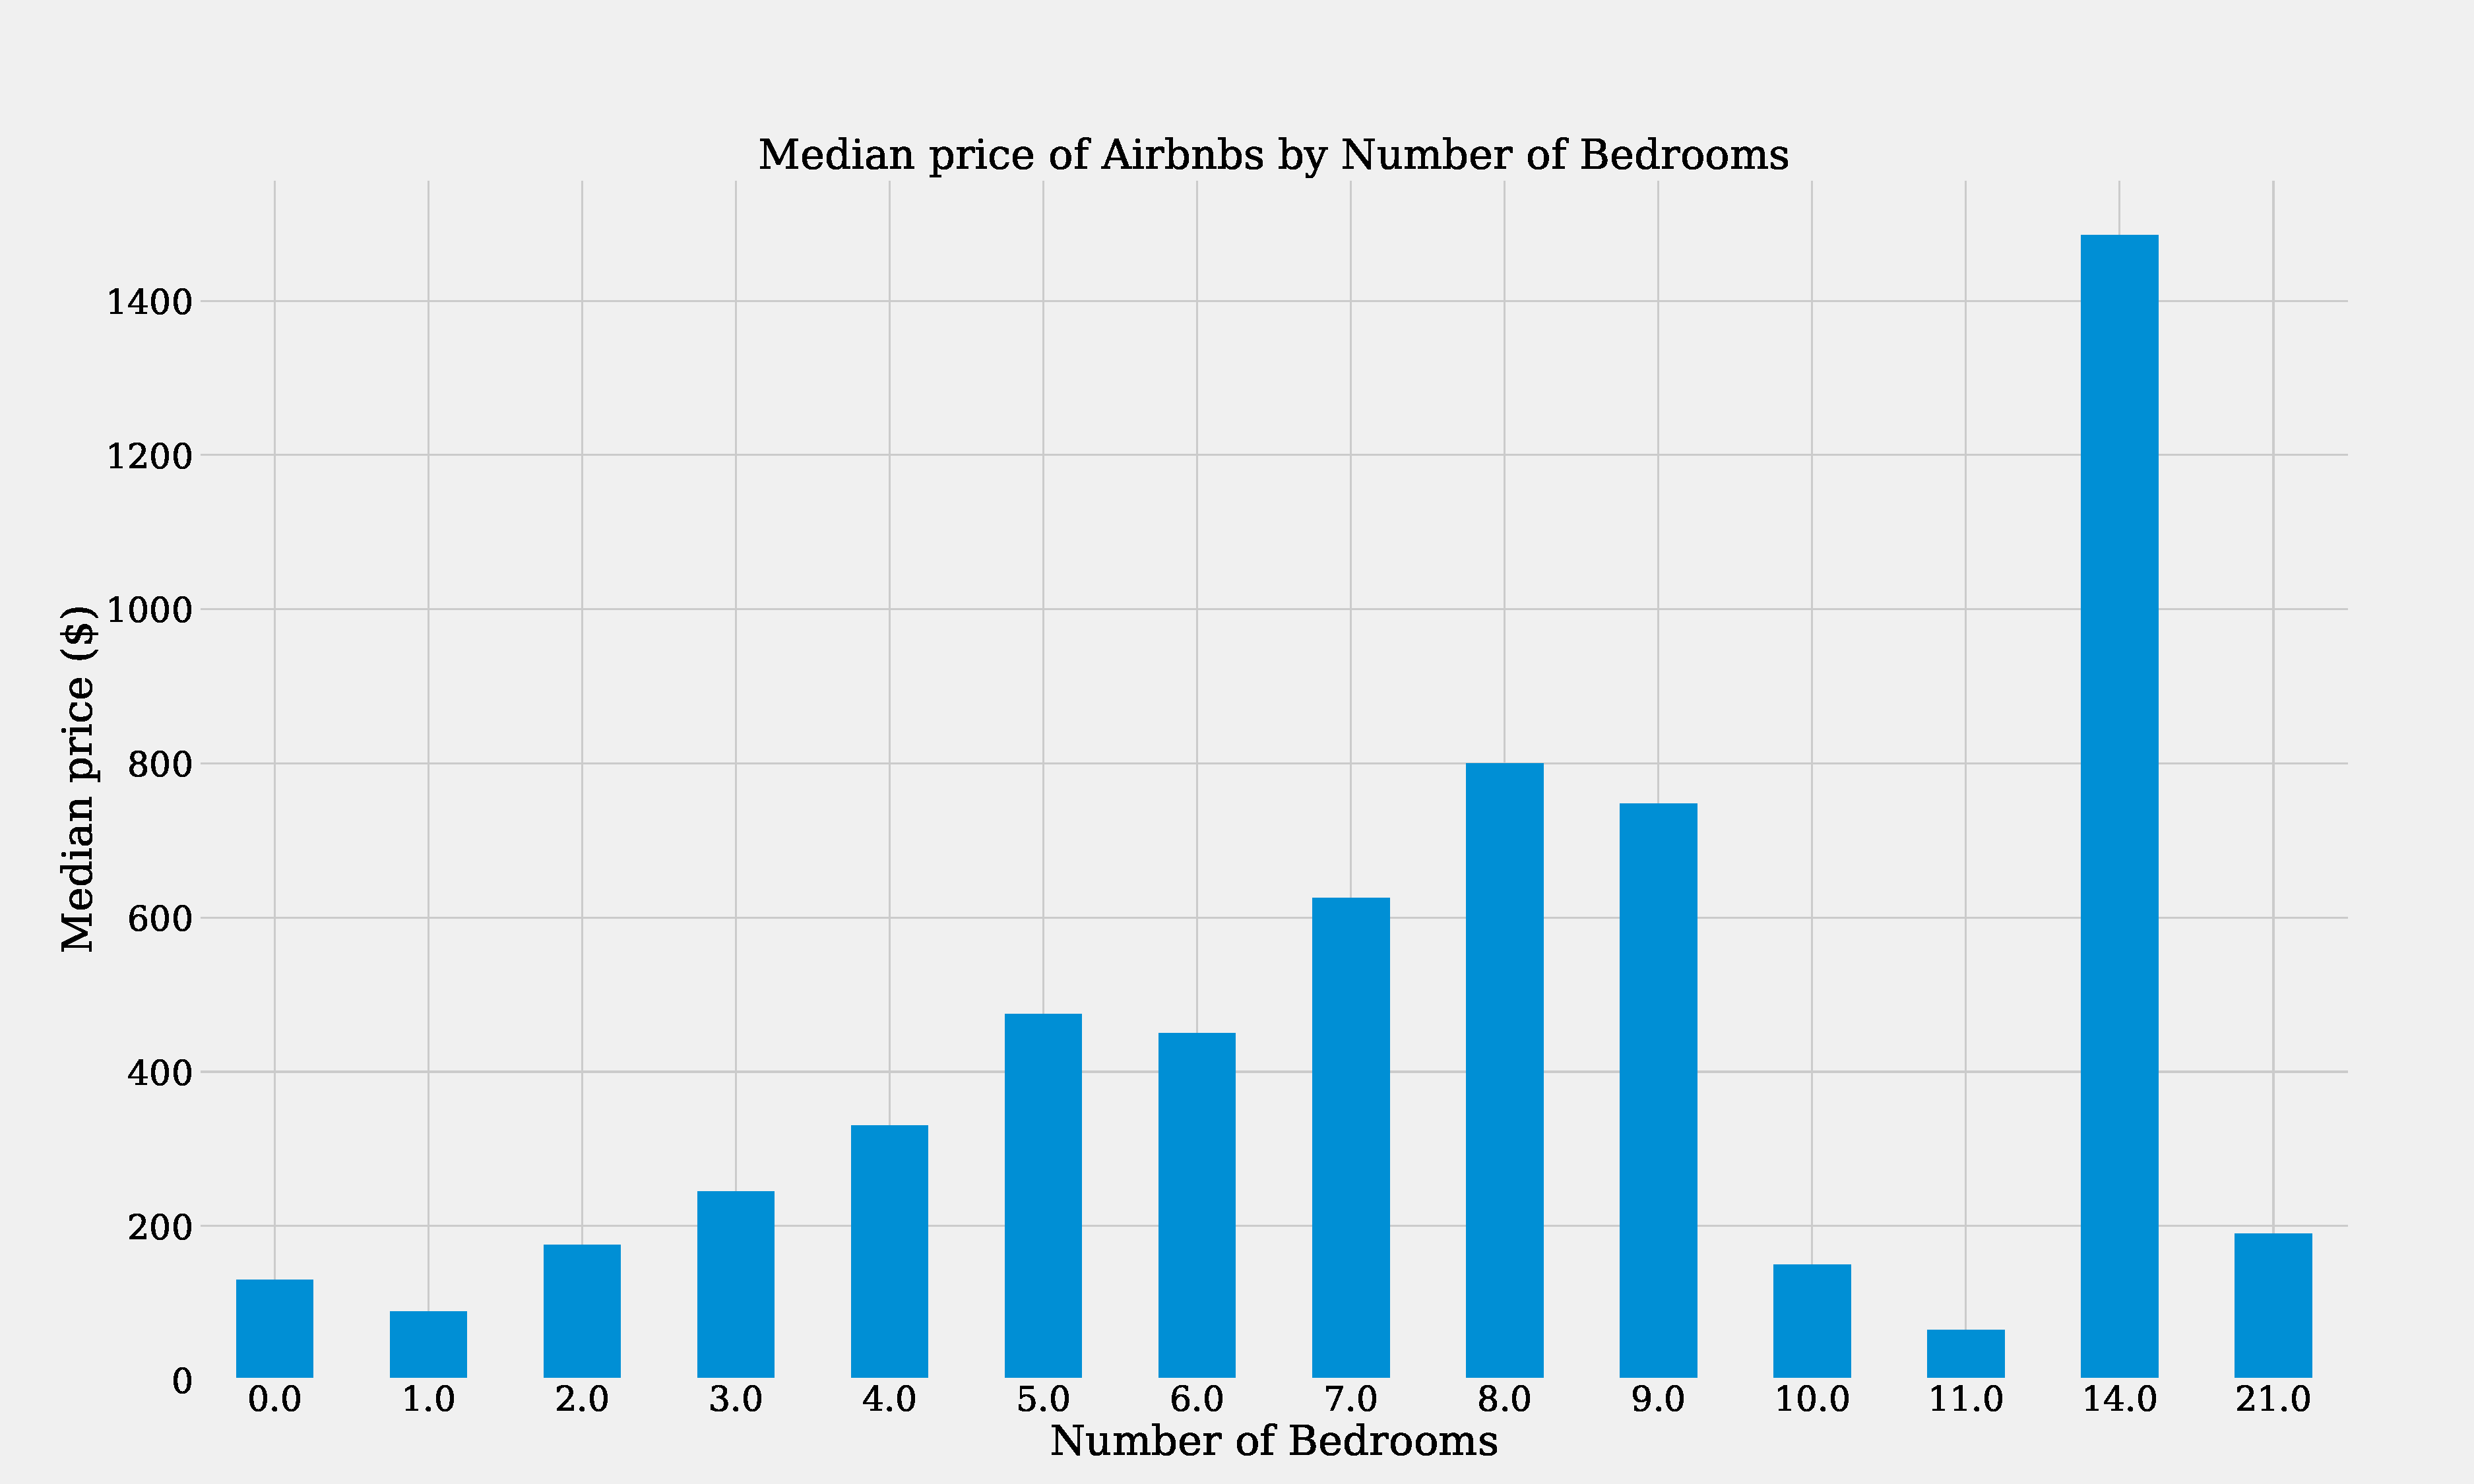
\includegraphics[width=\textwidth]{median-price-by-bedrooms.pdf}
    \caption{Median Price By Number of Bedrooms}
    \label{fig:median-price-by-bedrooms}
\end{figure}


\begin{figure}[H] \centering
    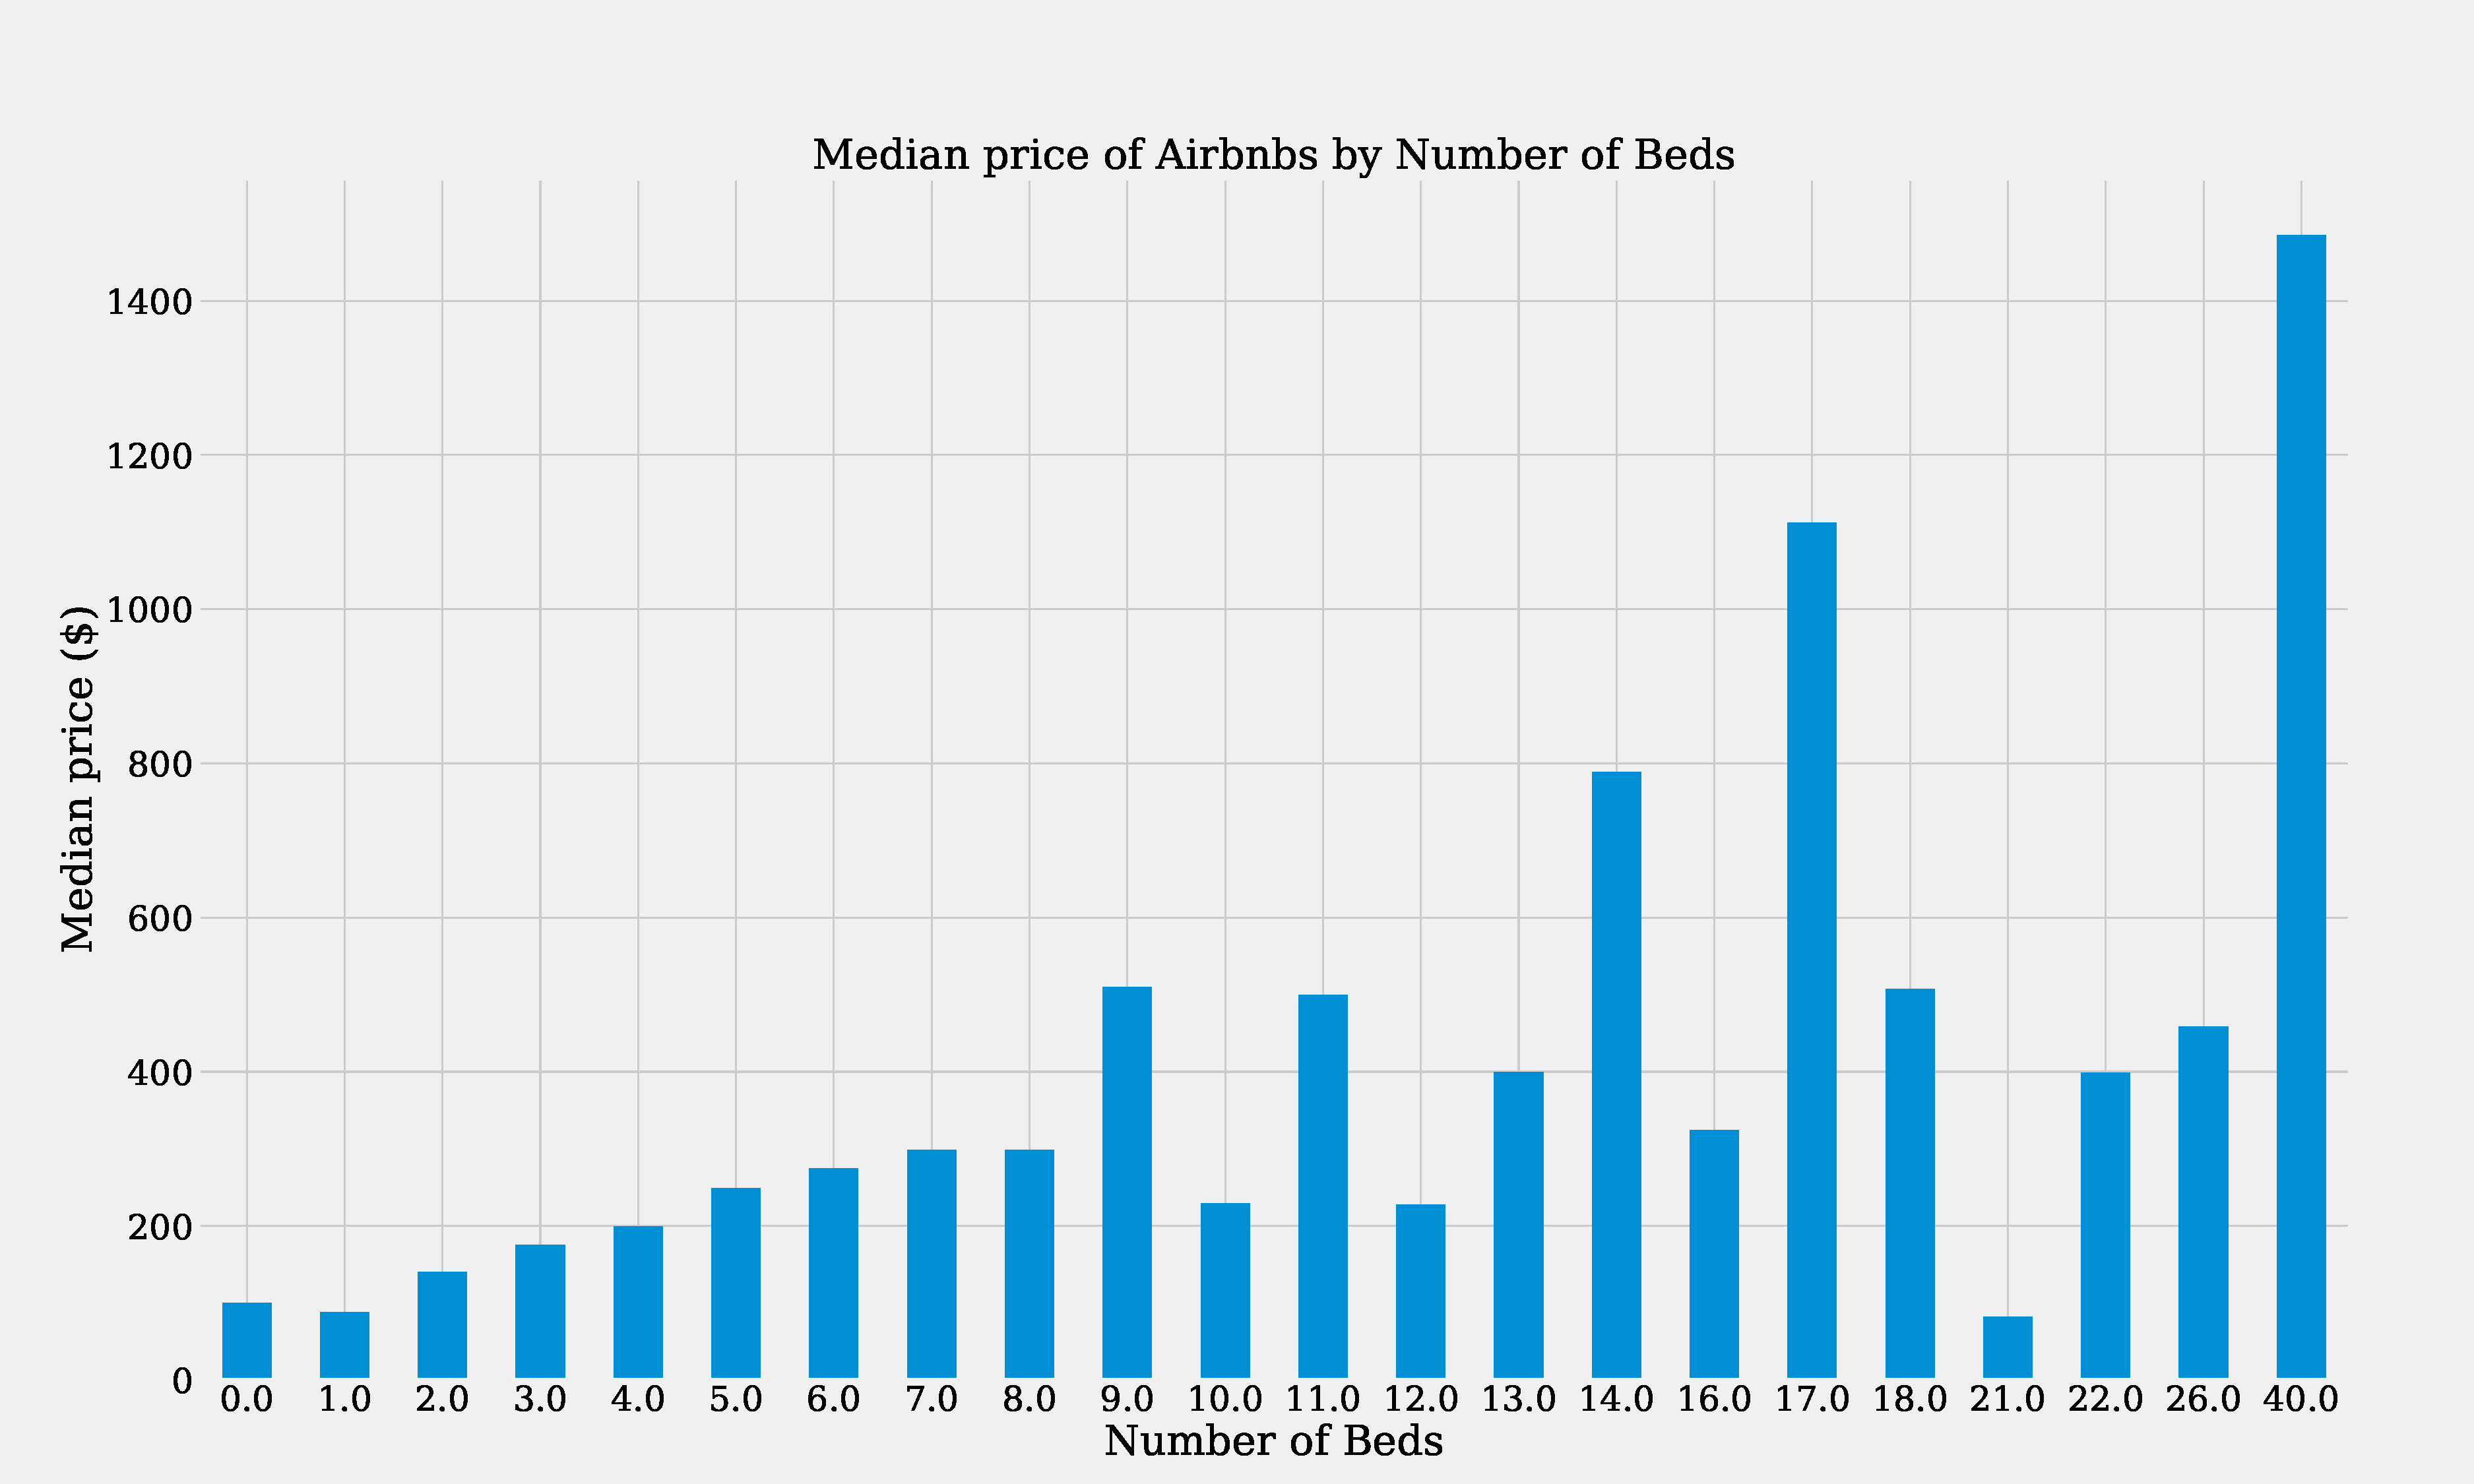
\includegraphics[width=\textwidth]{median-price-by-beds.pdf}
    \caption{Median Price By Number of Beds}
    \label{fig:median-price-by-beds}
\end{figure}

% ------------------------------

% Amenity Group 1
\begin{figure}[H]
\centering
    \caption{Elevator and Bed Linen}
    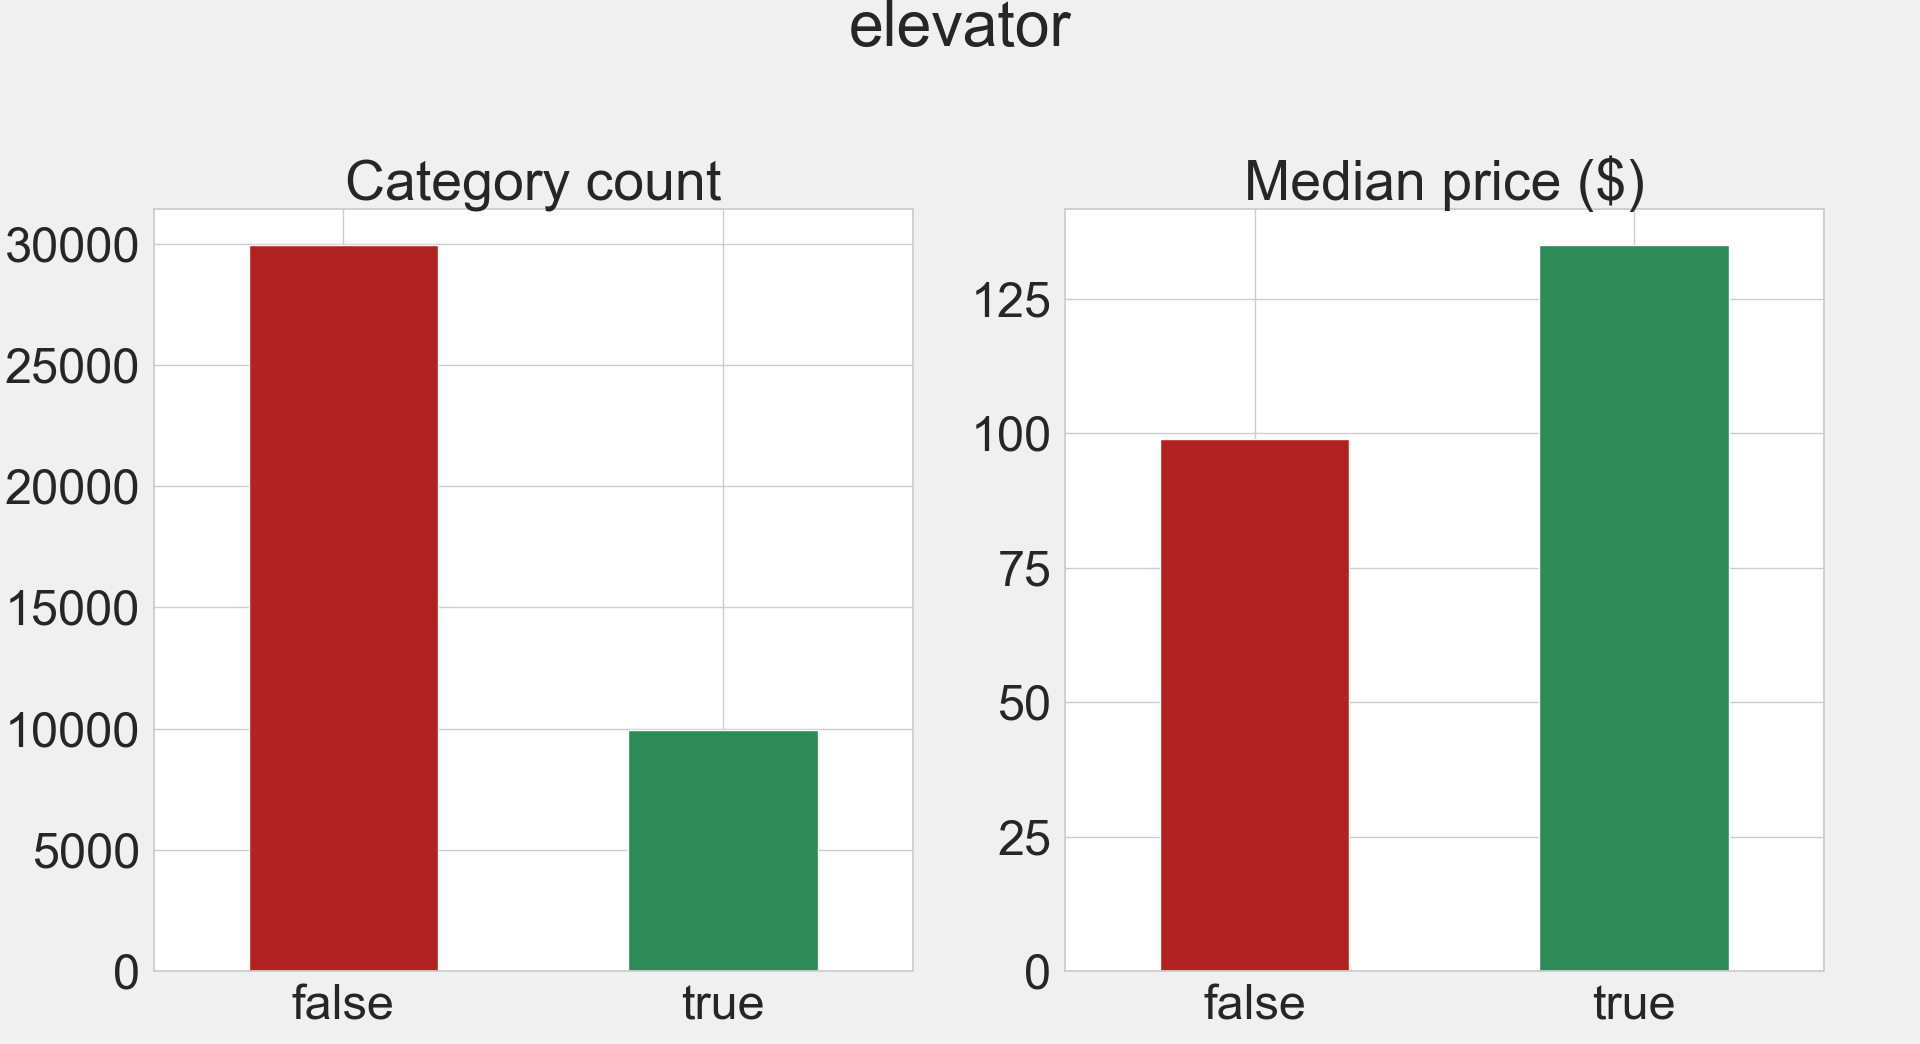
\includegraphics[width=\linewidth]{figures/amenities/group1/elevator.png}
    %\caption{Caption 1}
    \vspace{0.3cm}
    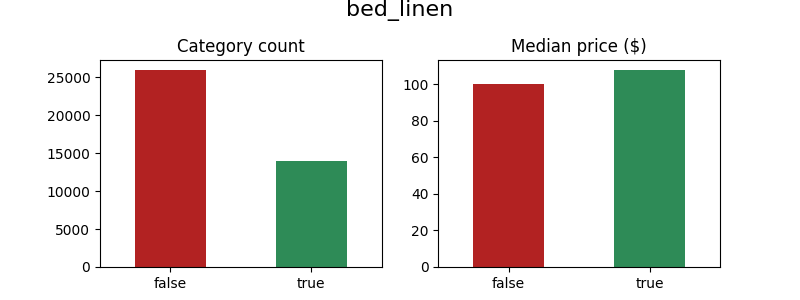
\includegraphics[width=\linewidth]{figures/amenities/group1/bed_linen.png}
    %\caption{Caption 2}
    \label{fig:elevator-and-bed-linen}
\end{figure}


\begin{figure}[H]
\centering
\caption{White Goods and Pets Allowed}
    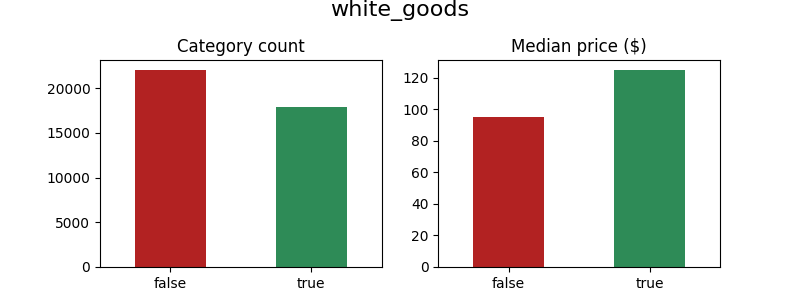
\includegraphics[width=\linewidth]{figures/amenities/group1/white_goods.png}
    %\caption{Caption 1}
    \vspace{0.5cm}
    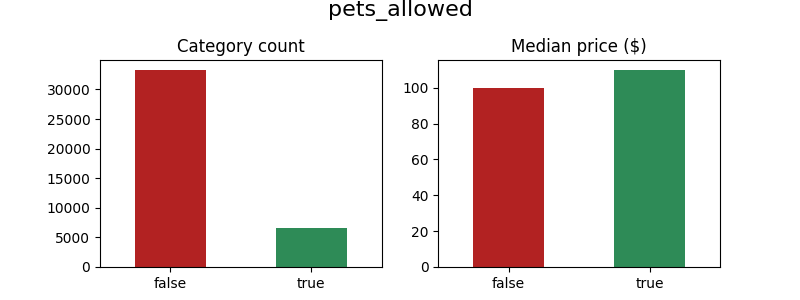
\includegraphics[width=\linewidth]{figures/amenities/group1/pets_allowed.png}
    %\caption{Caption 2}
    \label{fig:white-goods-and-pets-allowed}
    \
\end{figure}

\begin{figure}[H]
\centering
\caption{Self Check In and Coffee Machine}
    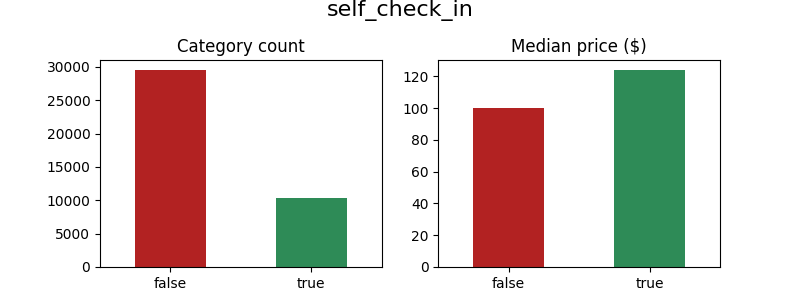
\includegraphics[width=\linewidth]{figures/amenities/group1/self_checkin.png}
    %\caption{Caption 1}
    \vspace{0.5cm}
    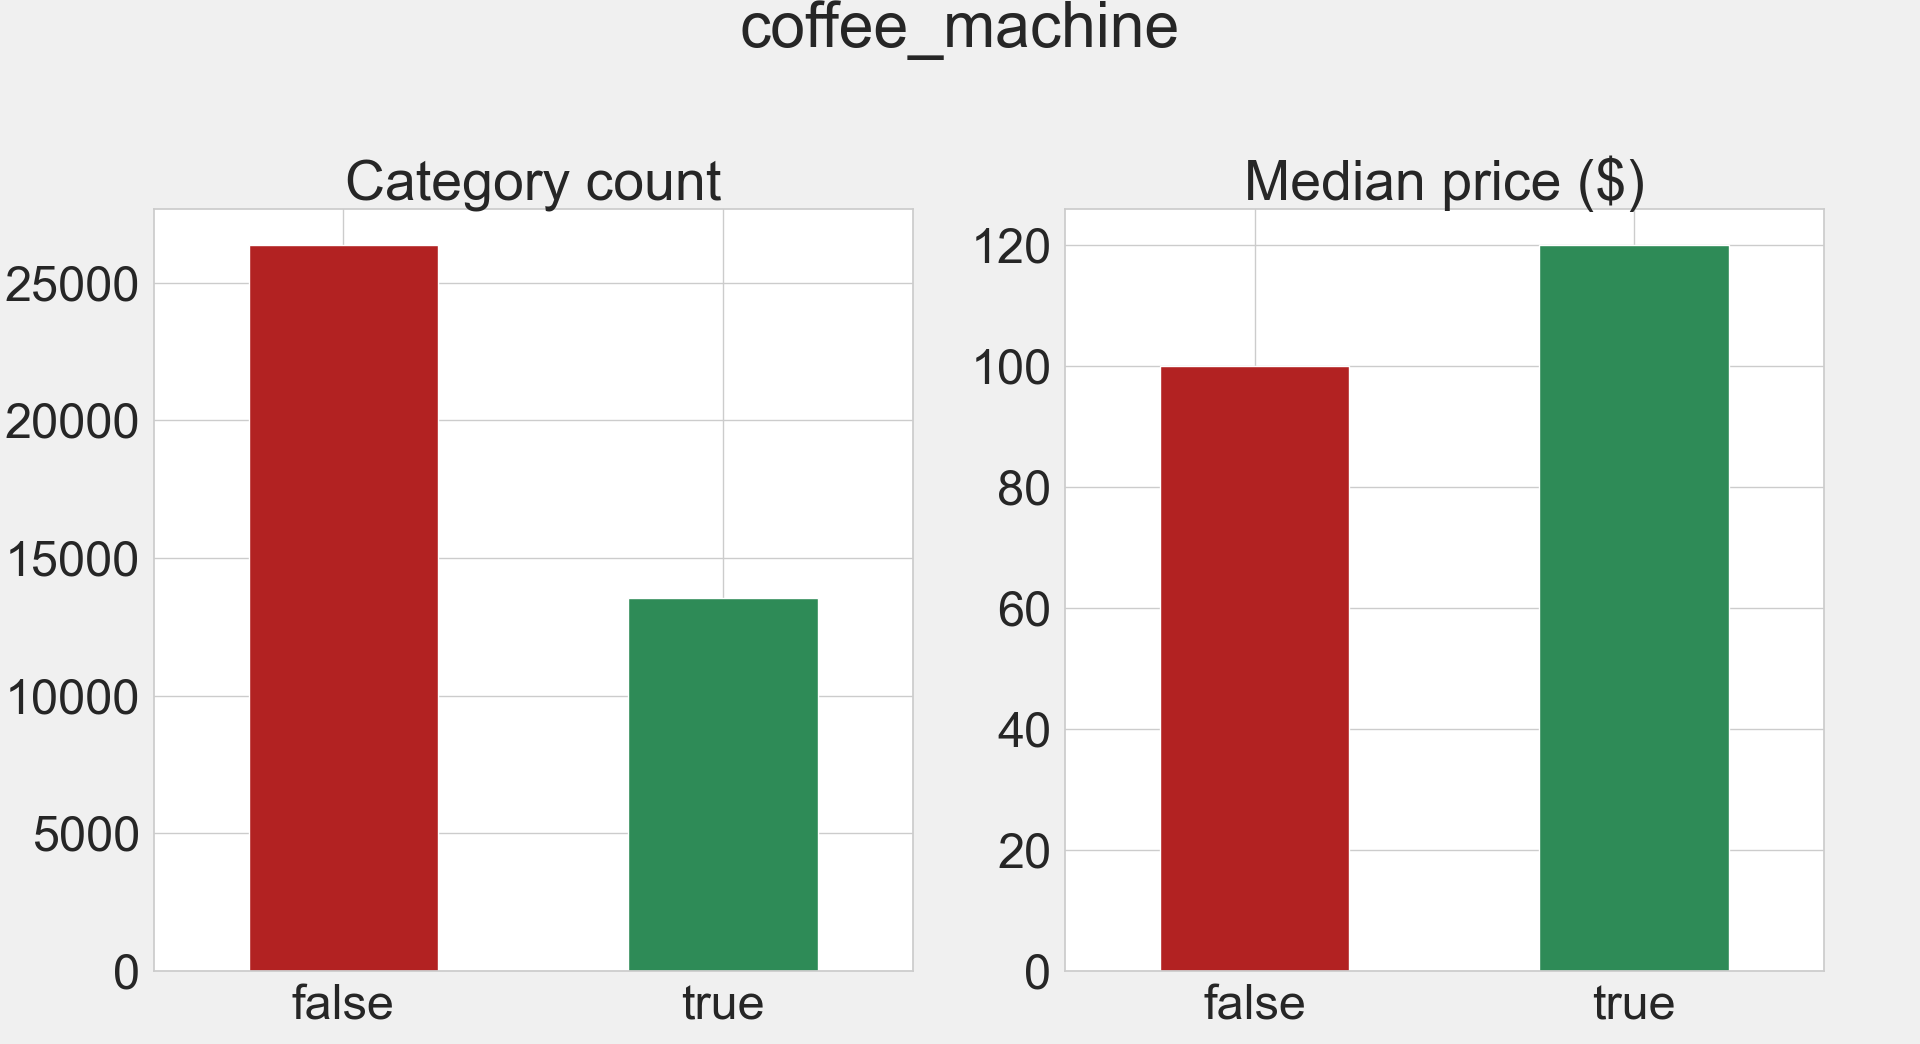
\includegraphics[width=\linewidth]{figures/amenities/group1/coffee_machine.png}
    %\caption{Caption 2}
    \label{fig:self-checkin-and-coffee-machine}
\end{figure}

\begin{figure}[H]
    \centering
    \caption{Long Term Stays and Child Friendly}
    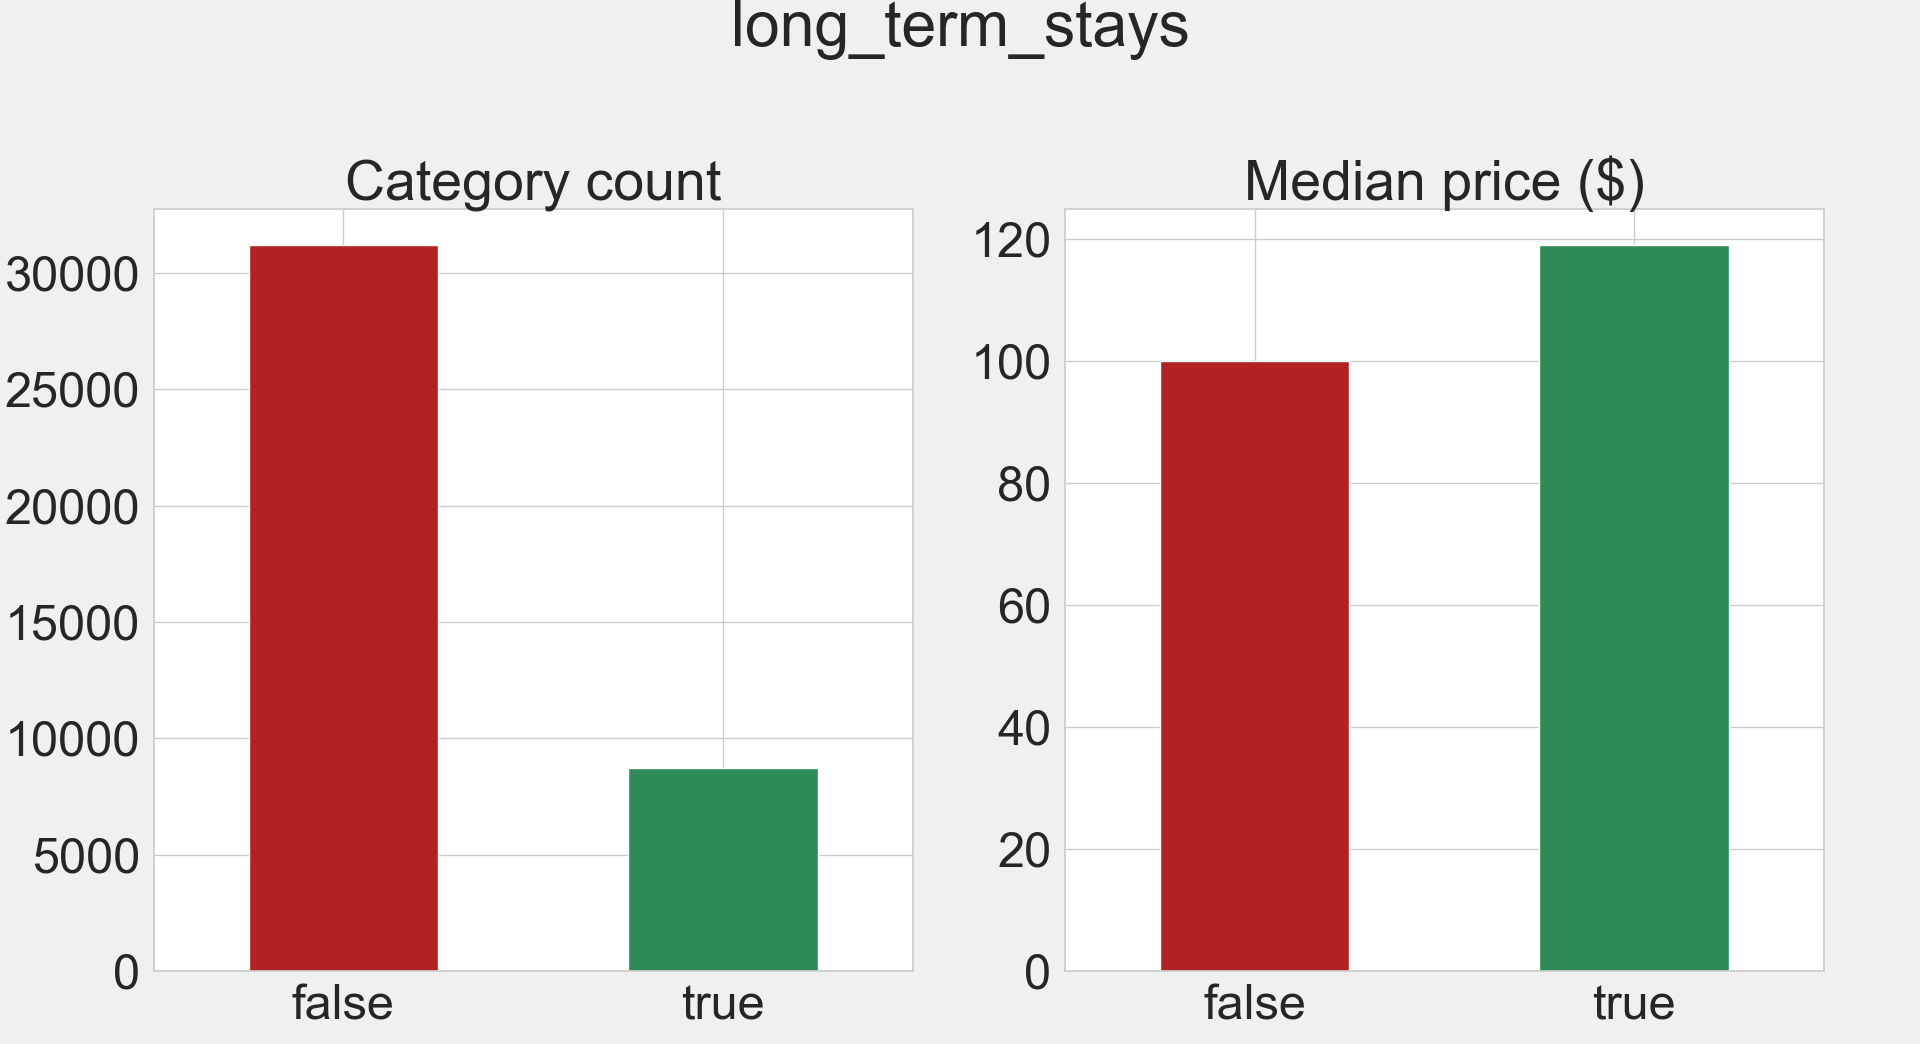
\includegraphics[width=\linewidth]{figures/amenities/group1/long_term_stays.png}
    %\caption{Caption 1}
    \vspace{0.5cm}
    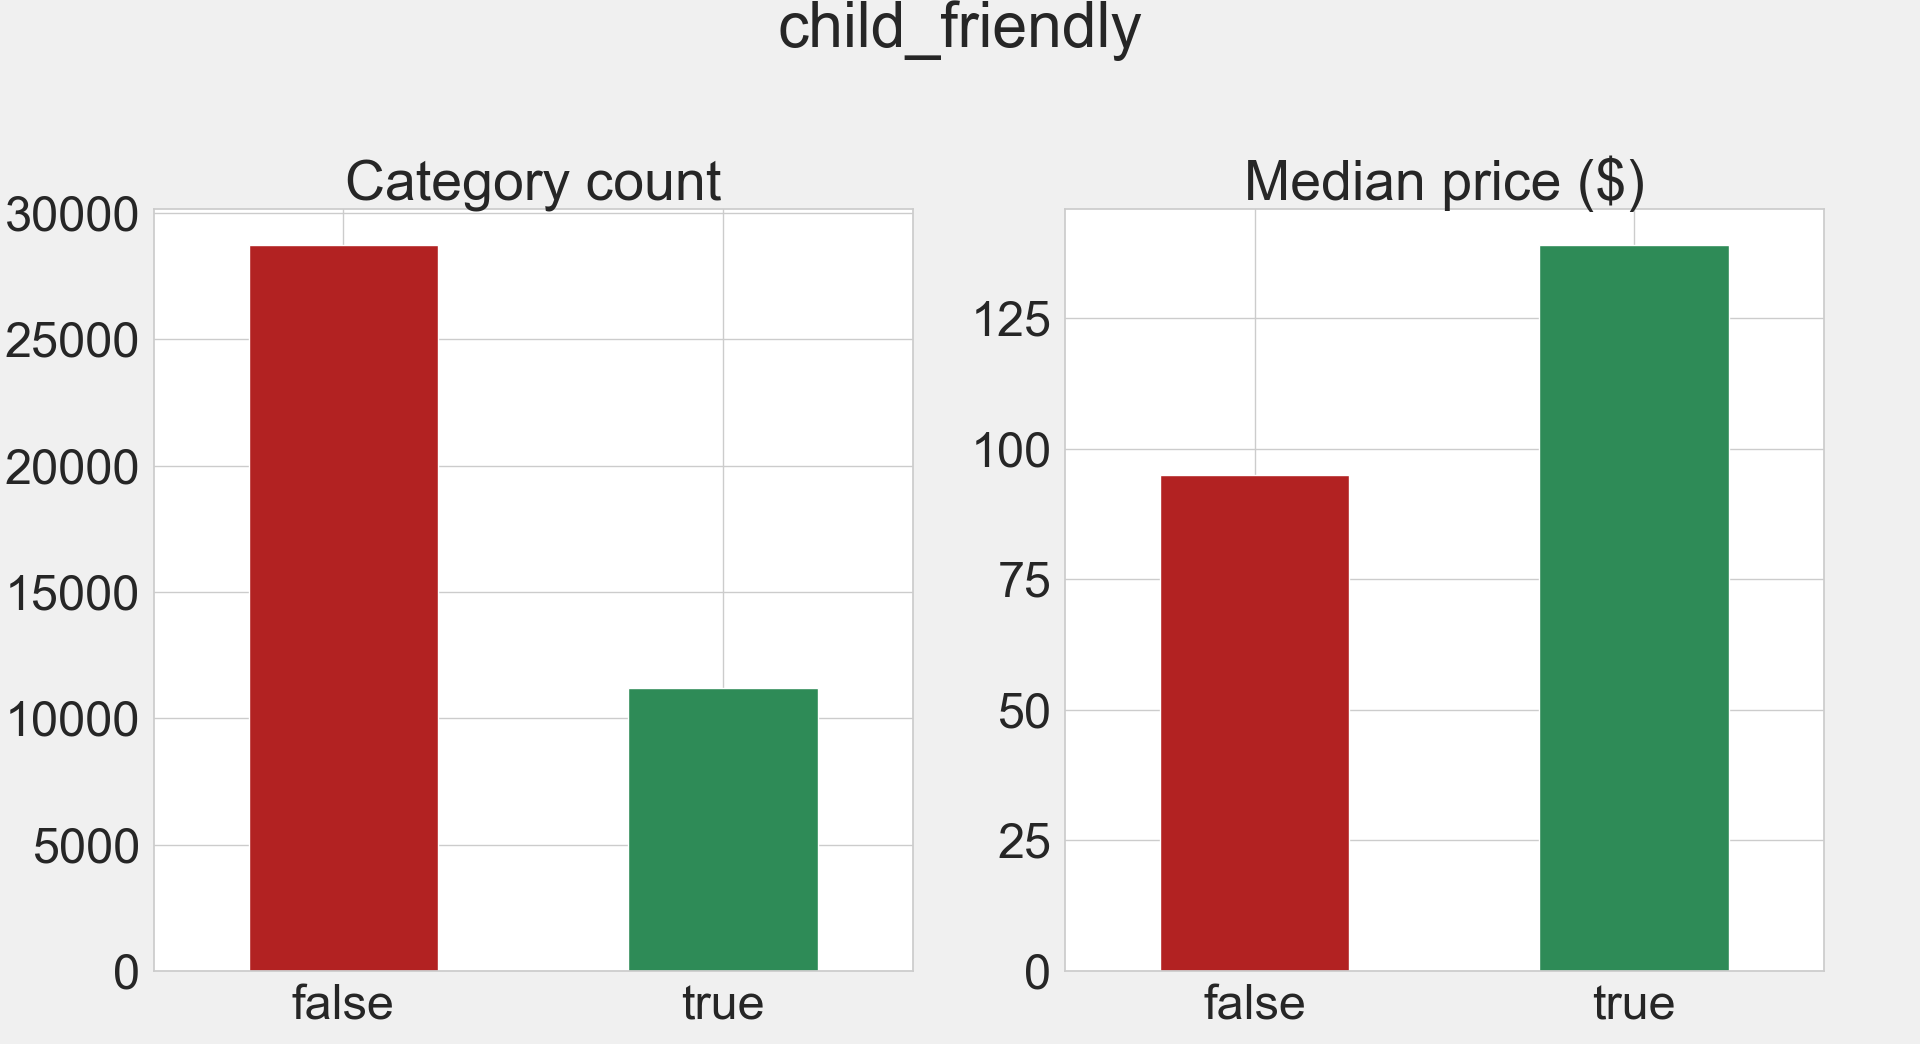
\includegraphics[width=\linewidth]{figures/amenities/group1/child_friendly.png}
    %\caption{Caption 2}
    \label{fig:long-term-stays-and-child-friendly}
\end{figure}

\begin{figure}[H]
\centering
\caption{Private Entrance and Cooking Basics}
    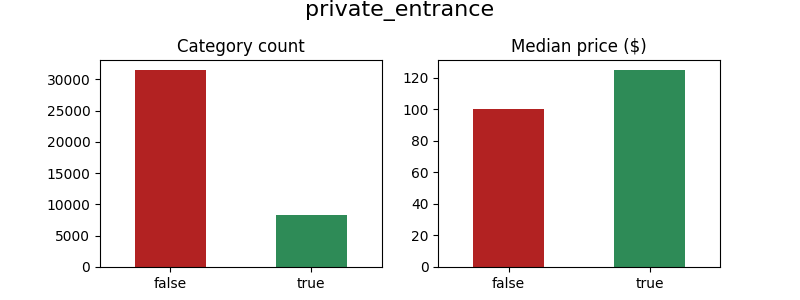
\includegraphics[width=\linewidth]{figures/amenities/group1/private_entrance.png}
    %\caption{Caption 1}
    \vspace{0.5cm}
    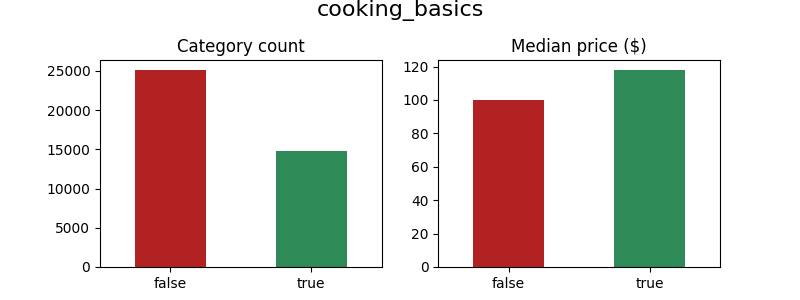
\includegraphics[width=\linewidth]{figures/amenities/group1/cooking_basics.png}
    %\caption{Caption 2}
    \label{fig:private-entrance-and-cooking-basics}
\end{figure}


% Amenity Group 2
\begin{figure}[H]
\centering
\caption{TV and Internet}
    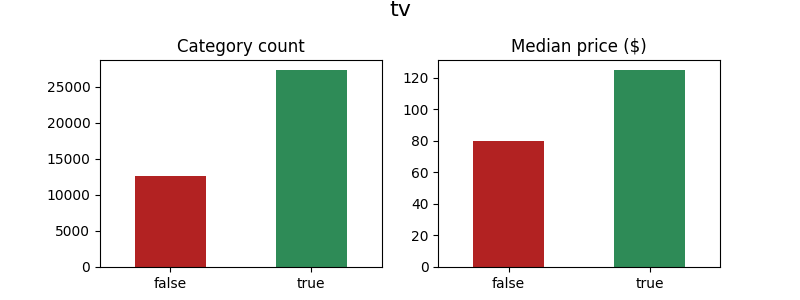
\includegraphics[width=\linewidth]{figures/amenities/group2/tv.png}
    %\caption{Caption 1}
    \vspace{0.5cm}
    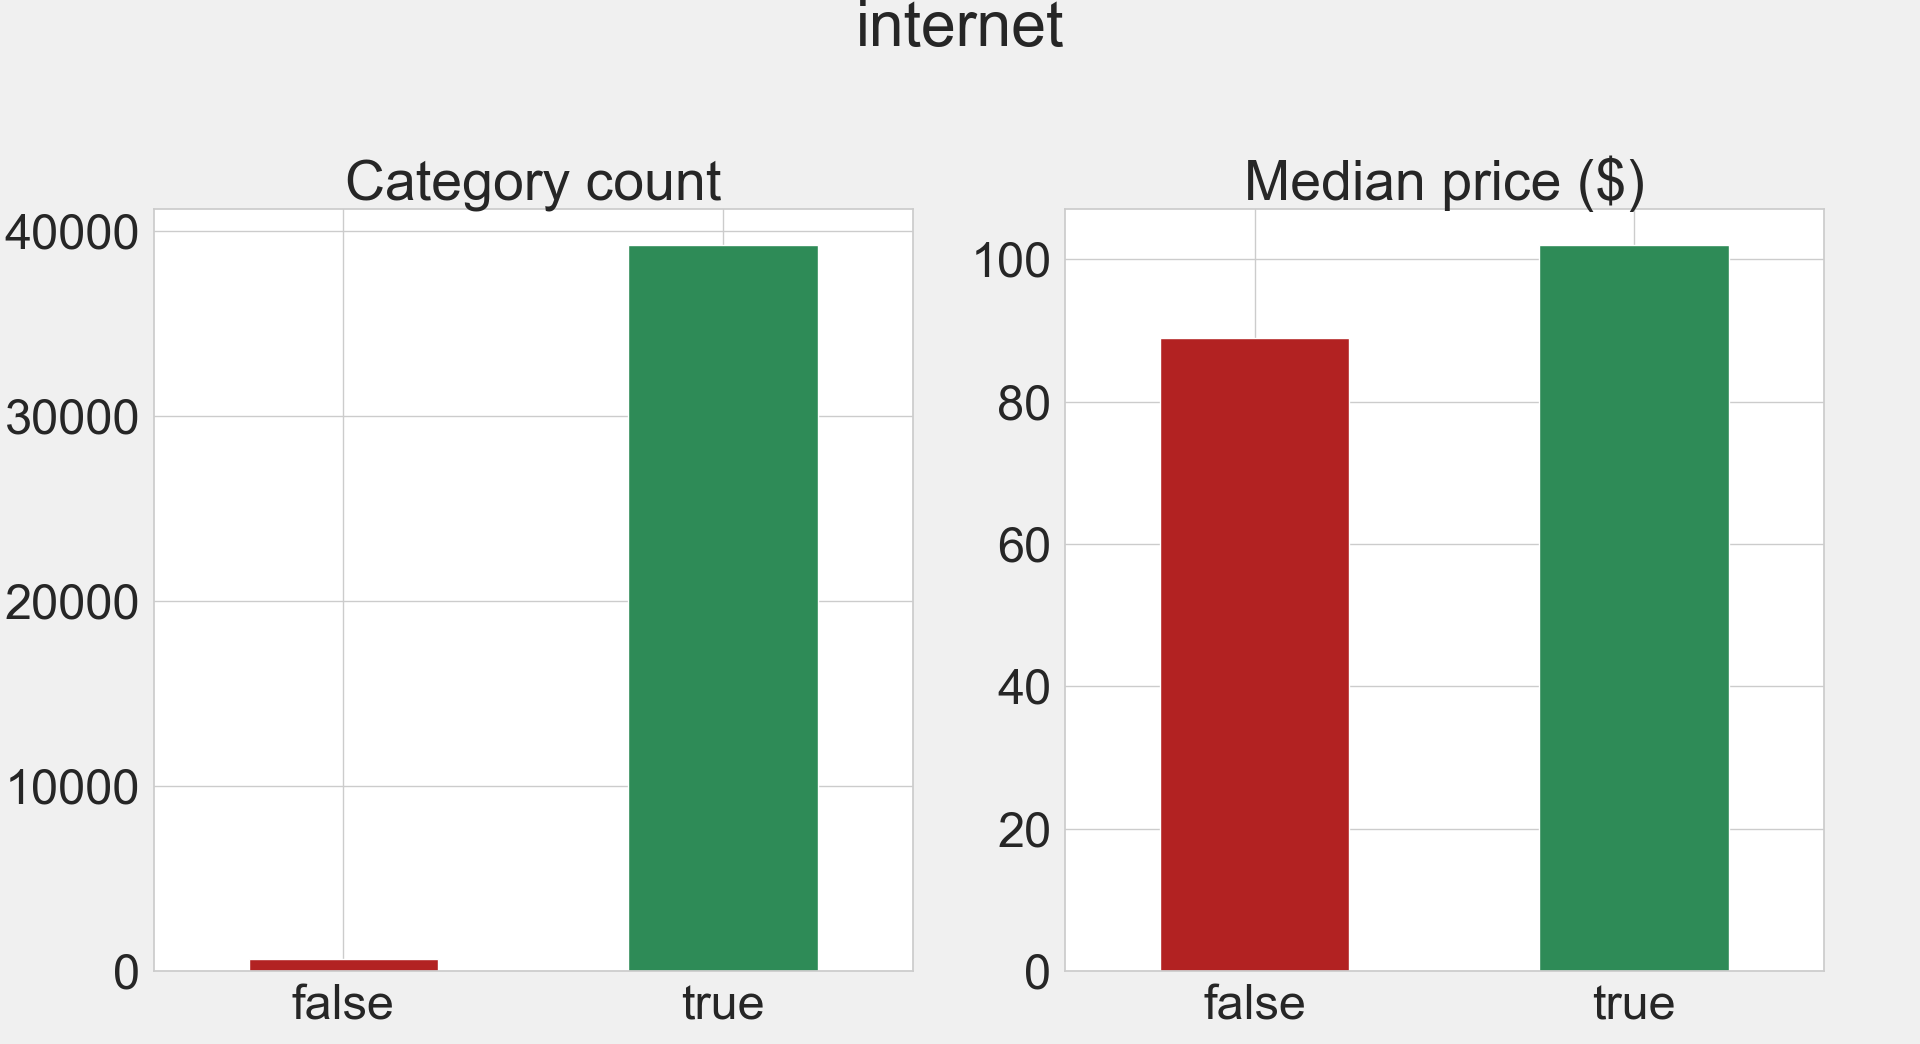
\includegraphics[width=\linewidth]{figures/amenities/group2/internet.png}
    %\caption{Caption 2}
    \label{fig:tv-and-internet}
\end{figure}

\begin{figure}[H]
\centering
    \caption{Air Conditioner}
    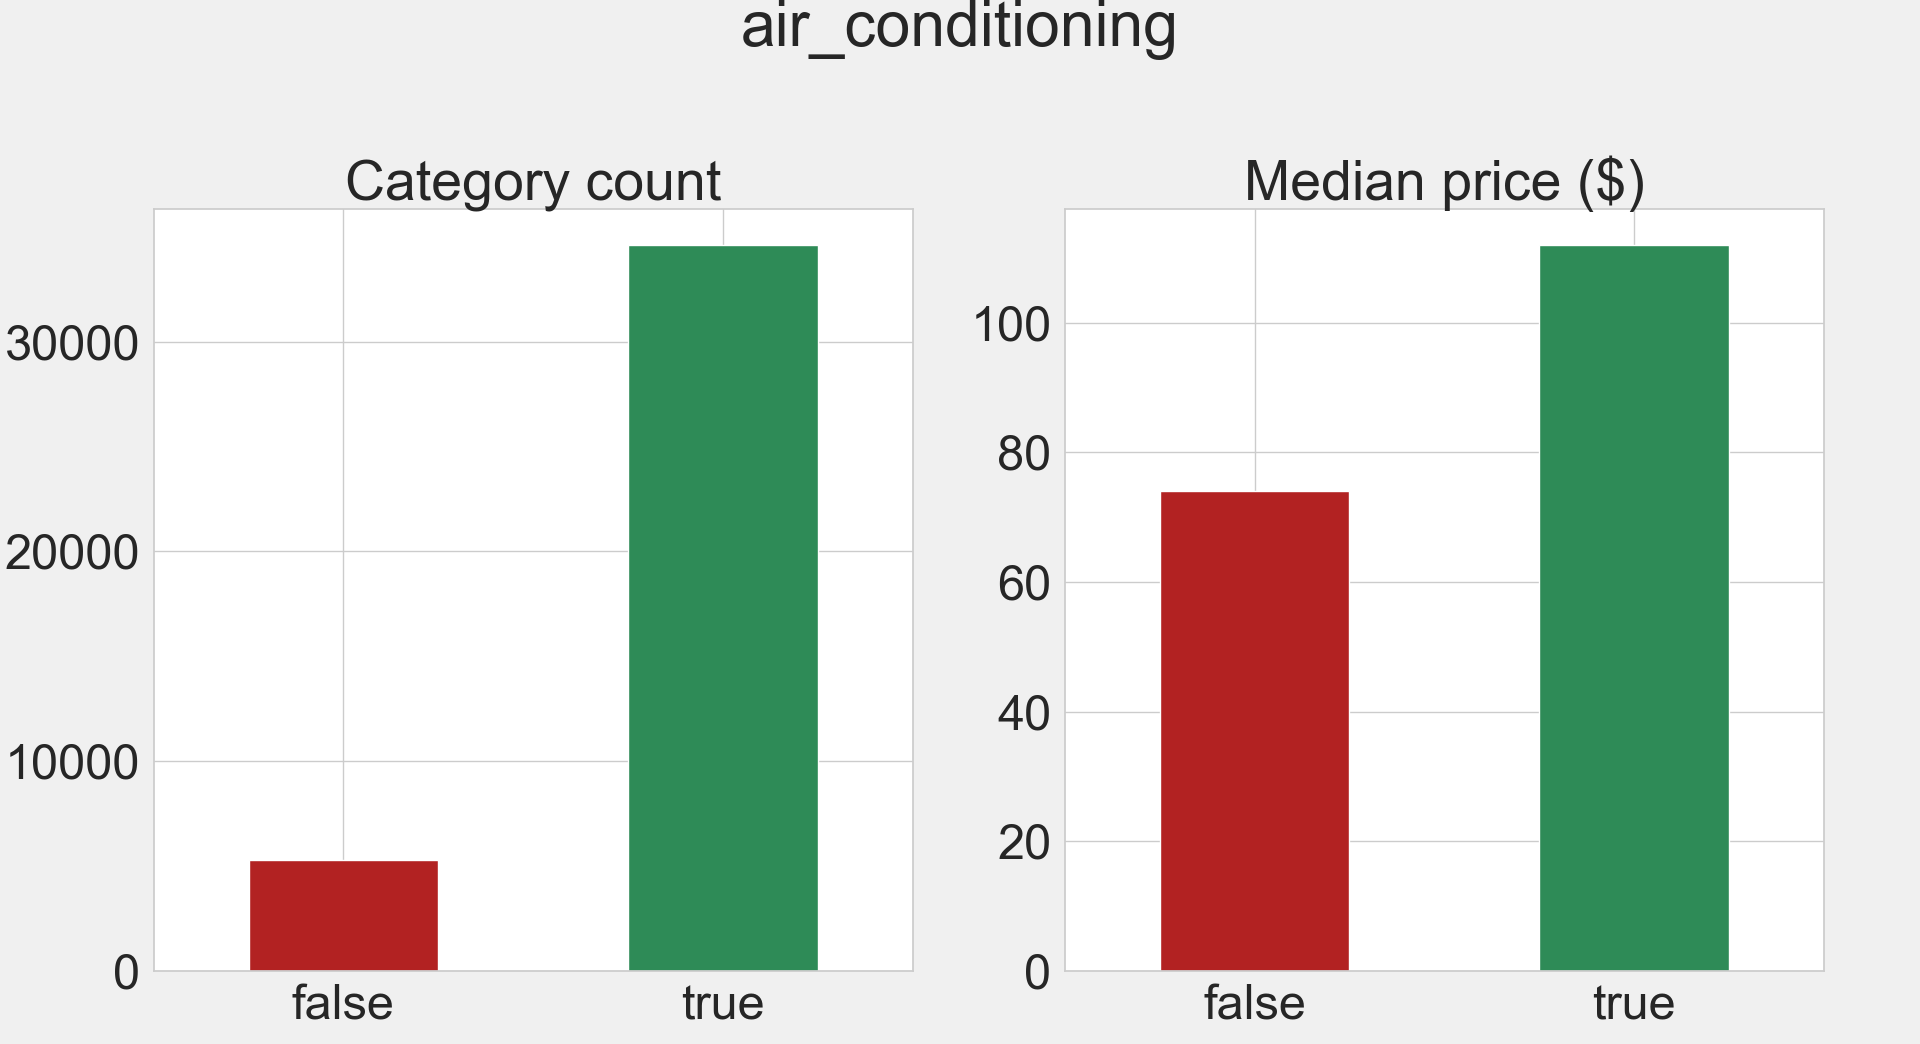
\includegraphics[width=\linewidth]{figures/amenities/group2/air_conditioning.png}
    \label{fig:air-conditioner}
\end{figure}

% Amenity Group 3
\begin{figure}[H]
\centering
    \caption{Parking and Host Greeting}
    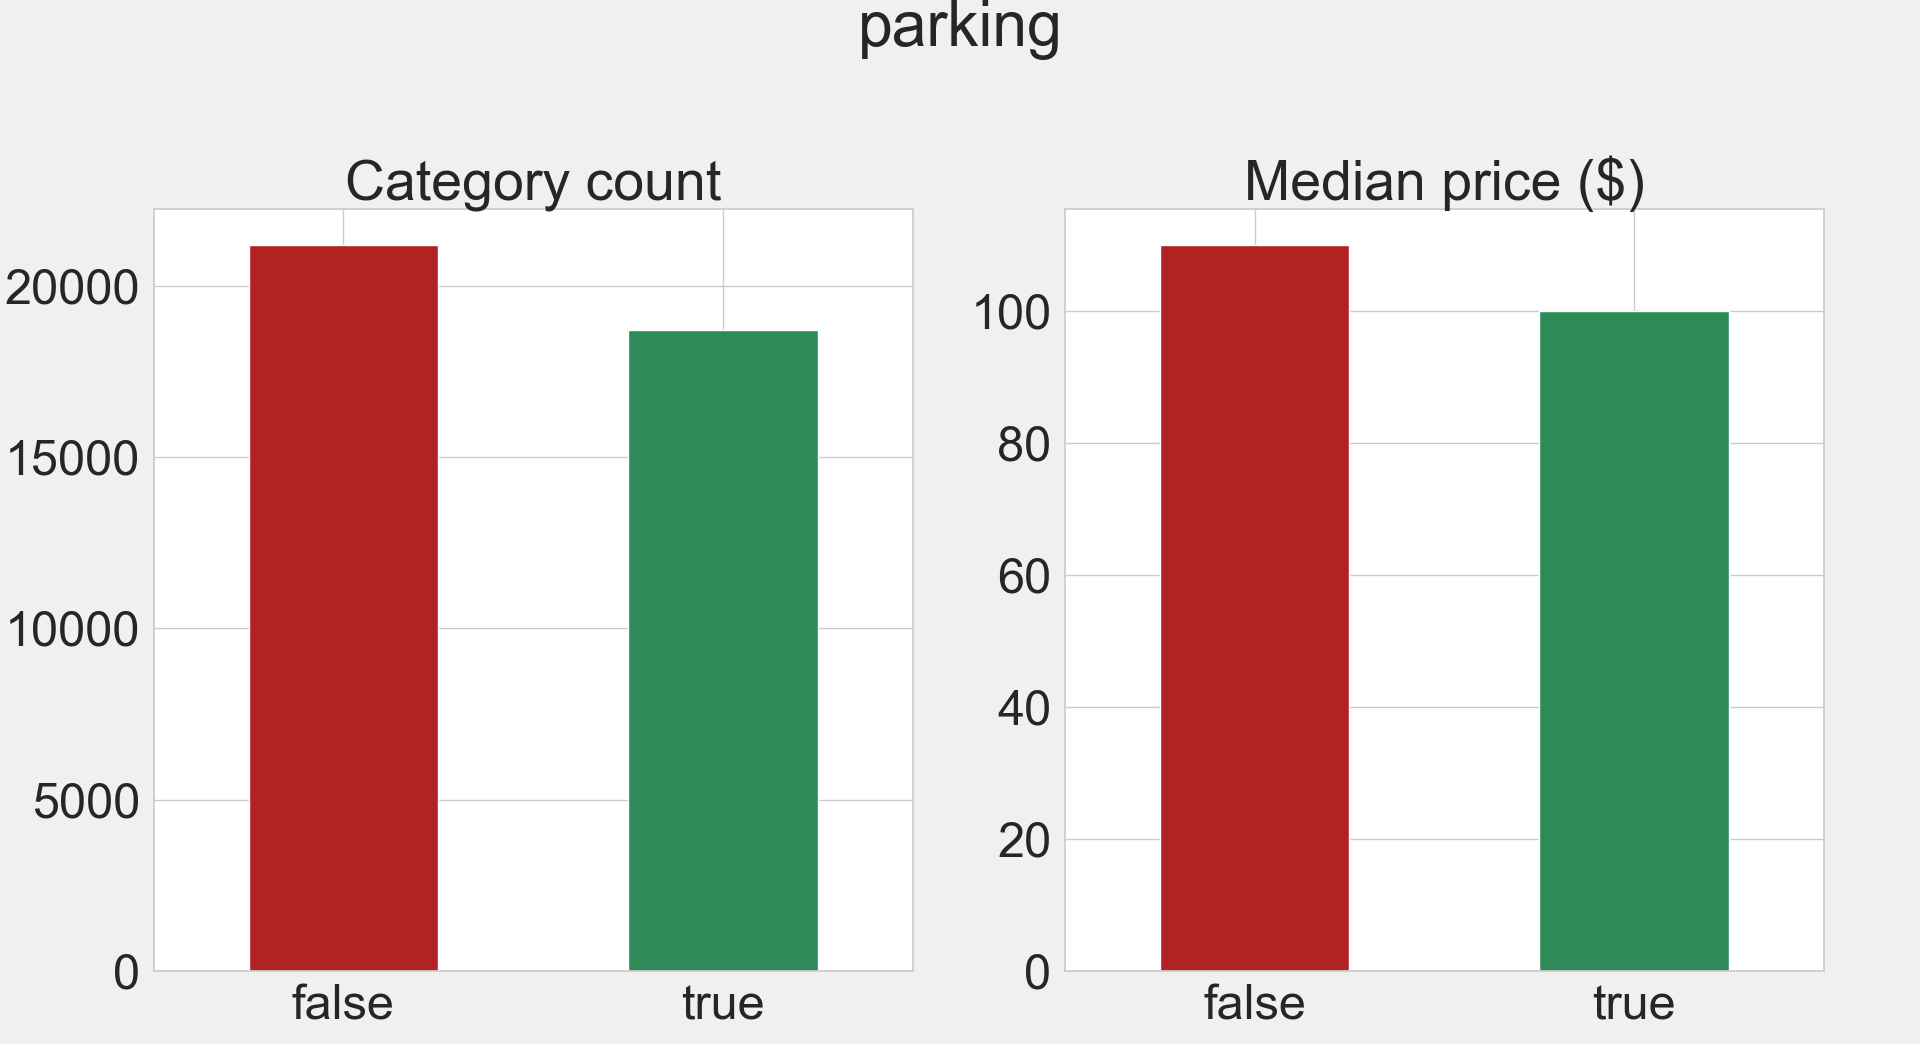
\includegraphics[width=\linewidth]{figures/amenities/group3/parking.png}
    \vspace{0.5cm}
    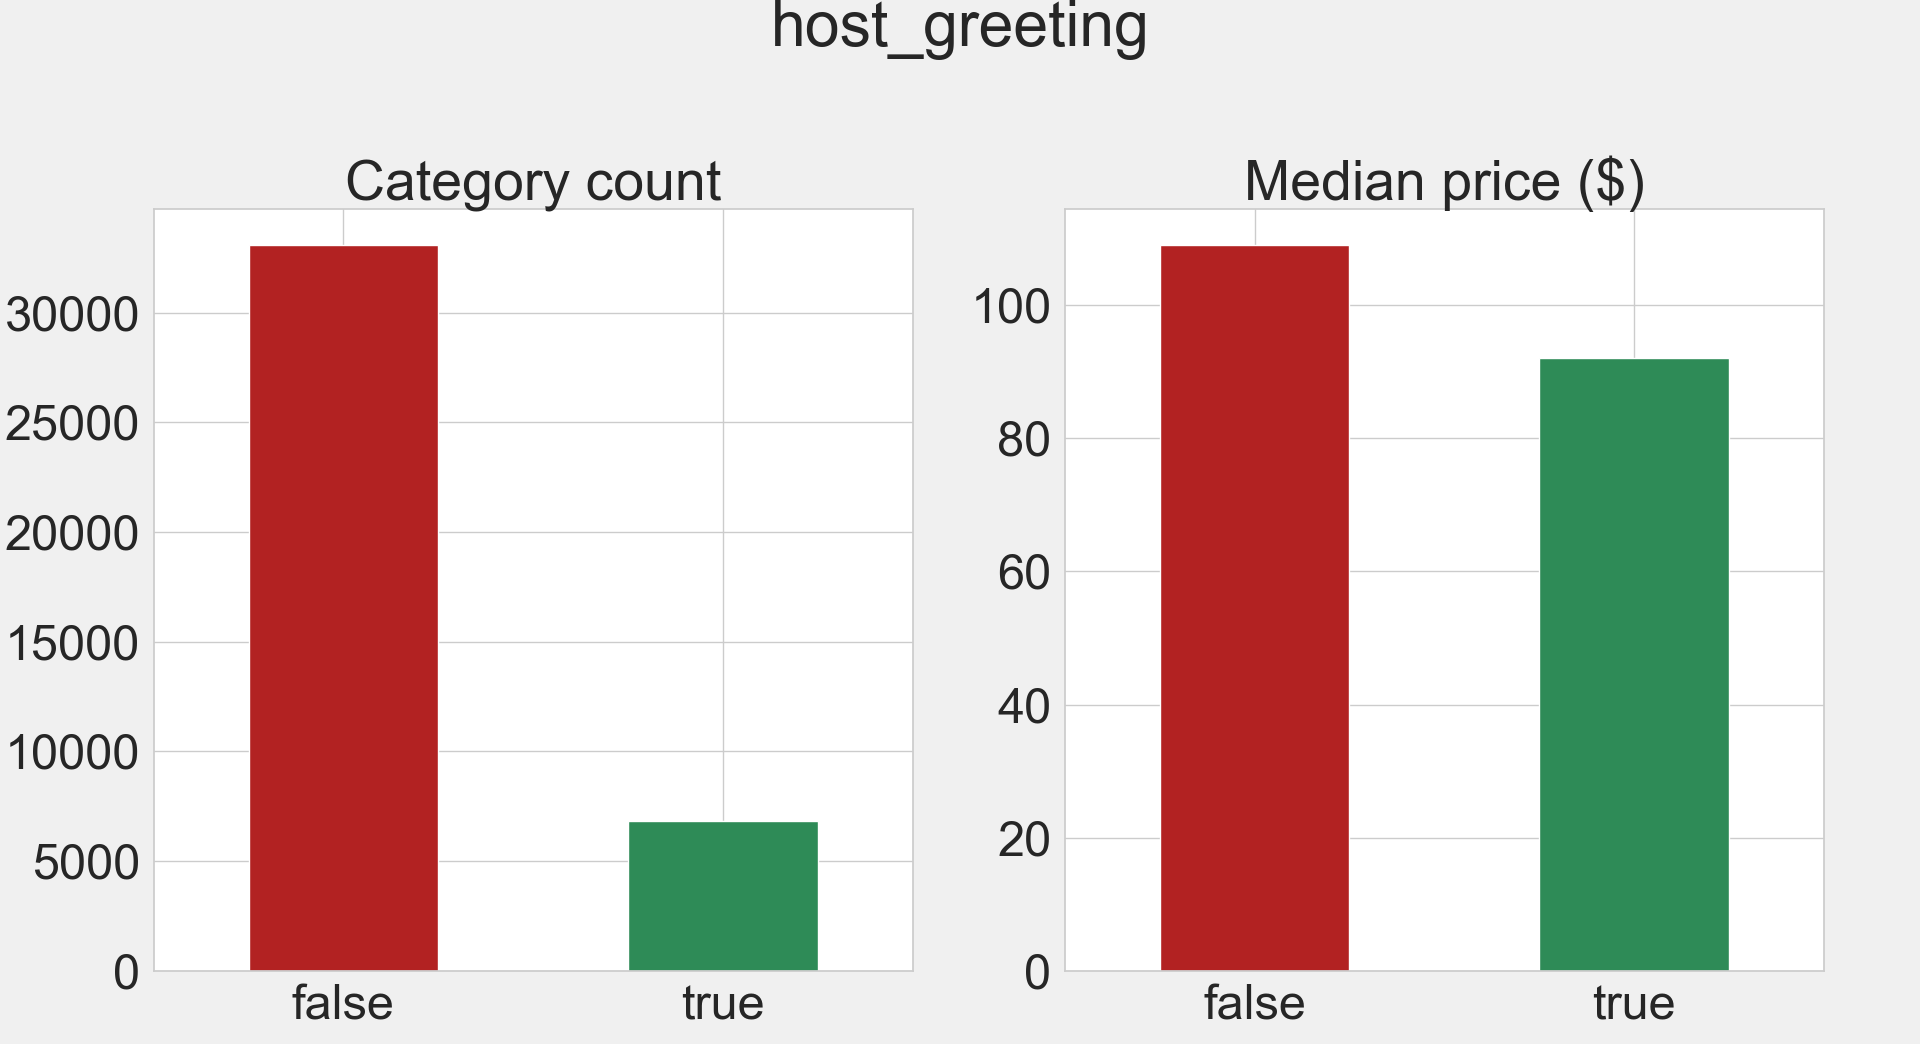
\includegraphics[width=\linewidth]{figures/amenities/group3/host_greetings.png}
    \label{fig:parking-and-host-greeting}
\end{figure}


\begin{figure}[H] \centering
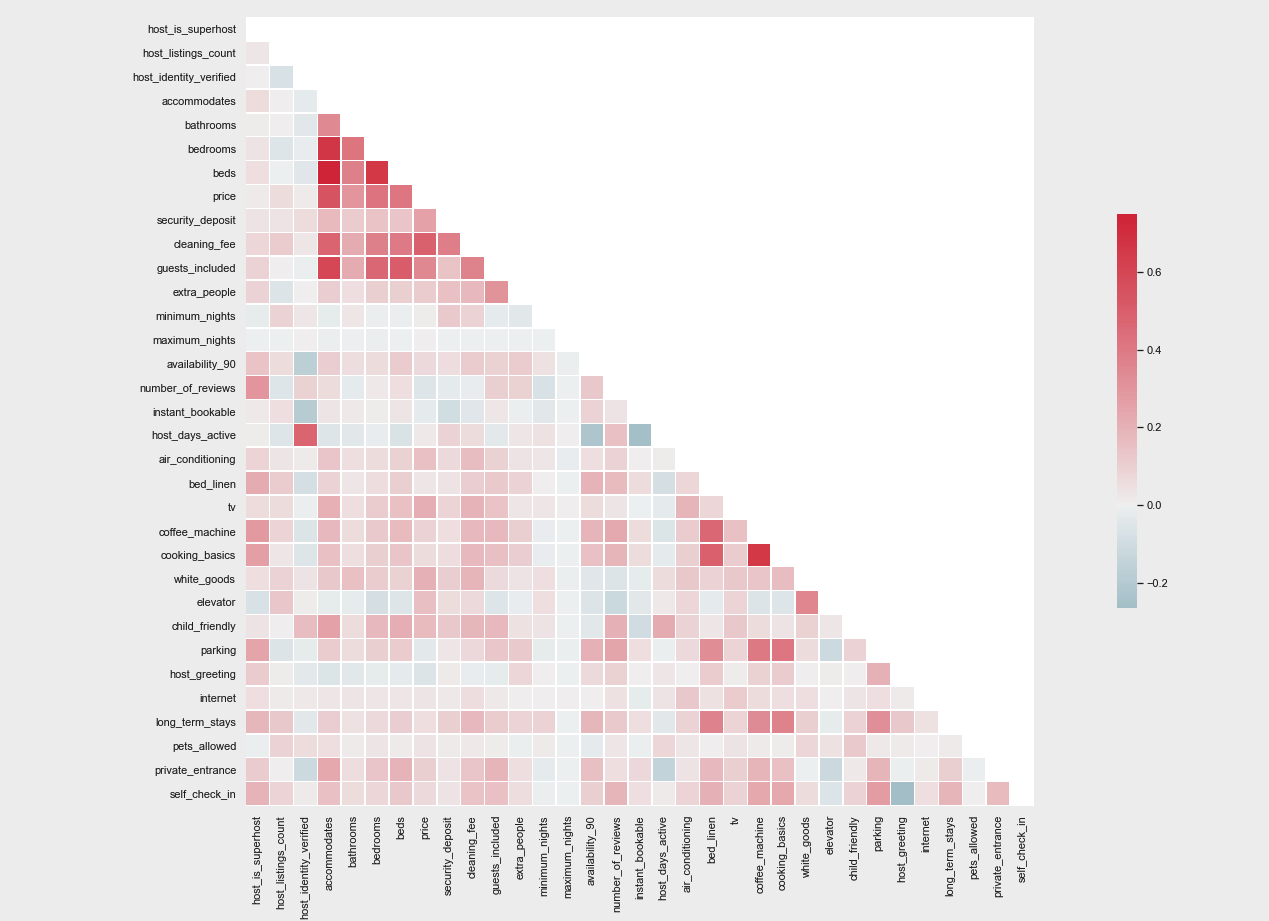
\includegraphics[width=\textwidth,keepaspectratio]{correlation-matrix.png}
\caption{Correlation Matrix}
\label{fig:correlation-matrix}
\end{figure}

\begin{figure}[H] \centering
\caption{Histogram of Feature Distribution}
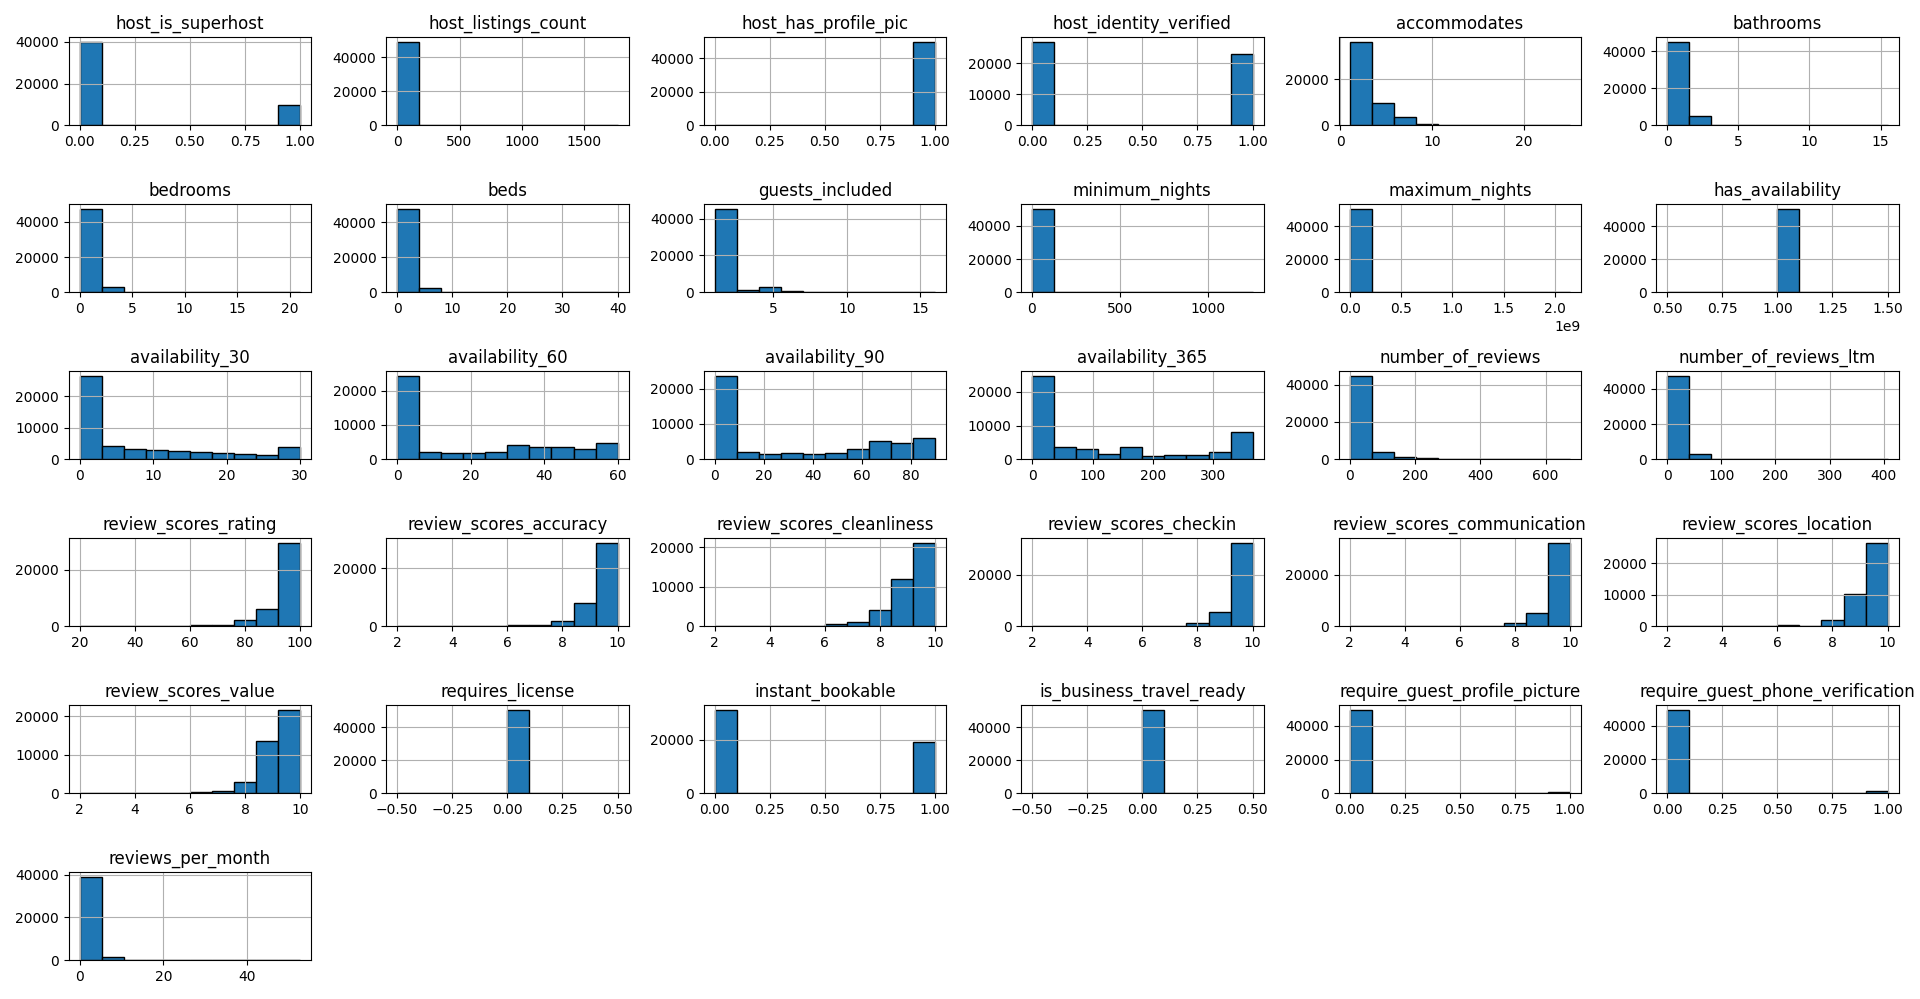
\includegraphics[width=\textwidth]{Figure_0_histogram.png}
\label{fig:histogram-feature-distribution}
\end{figure}

% from pre_processing.py
%Other than availability_90 and host_days_active, the remaining numerical
%features are all postively skewed and could benefit from log transformation.
\begin{figure}[H] \centering
\caption{Histogram of Numerical Feature Distribution Before Log Transform }
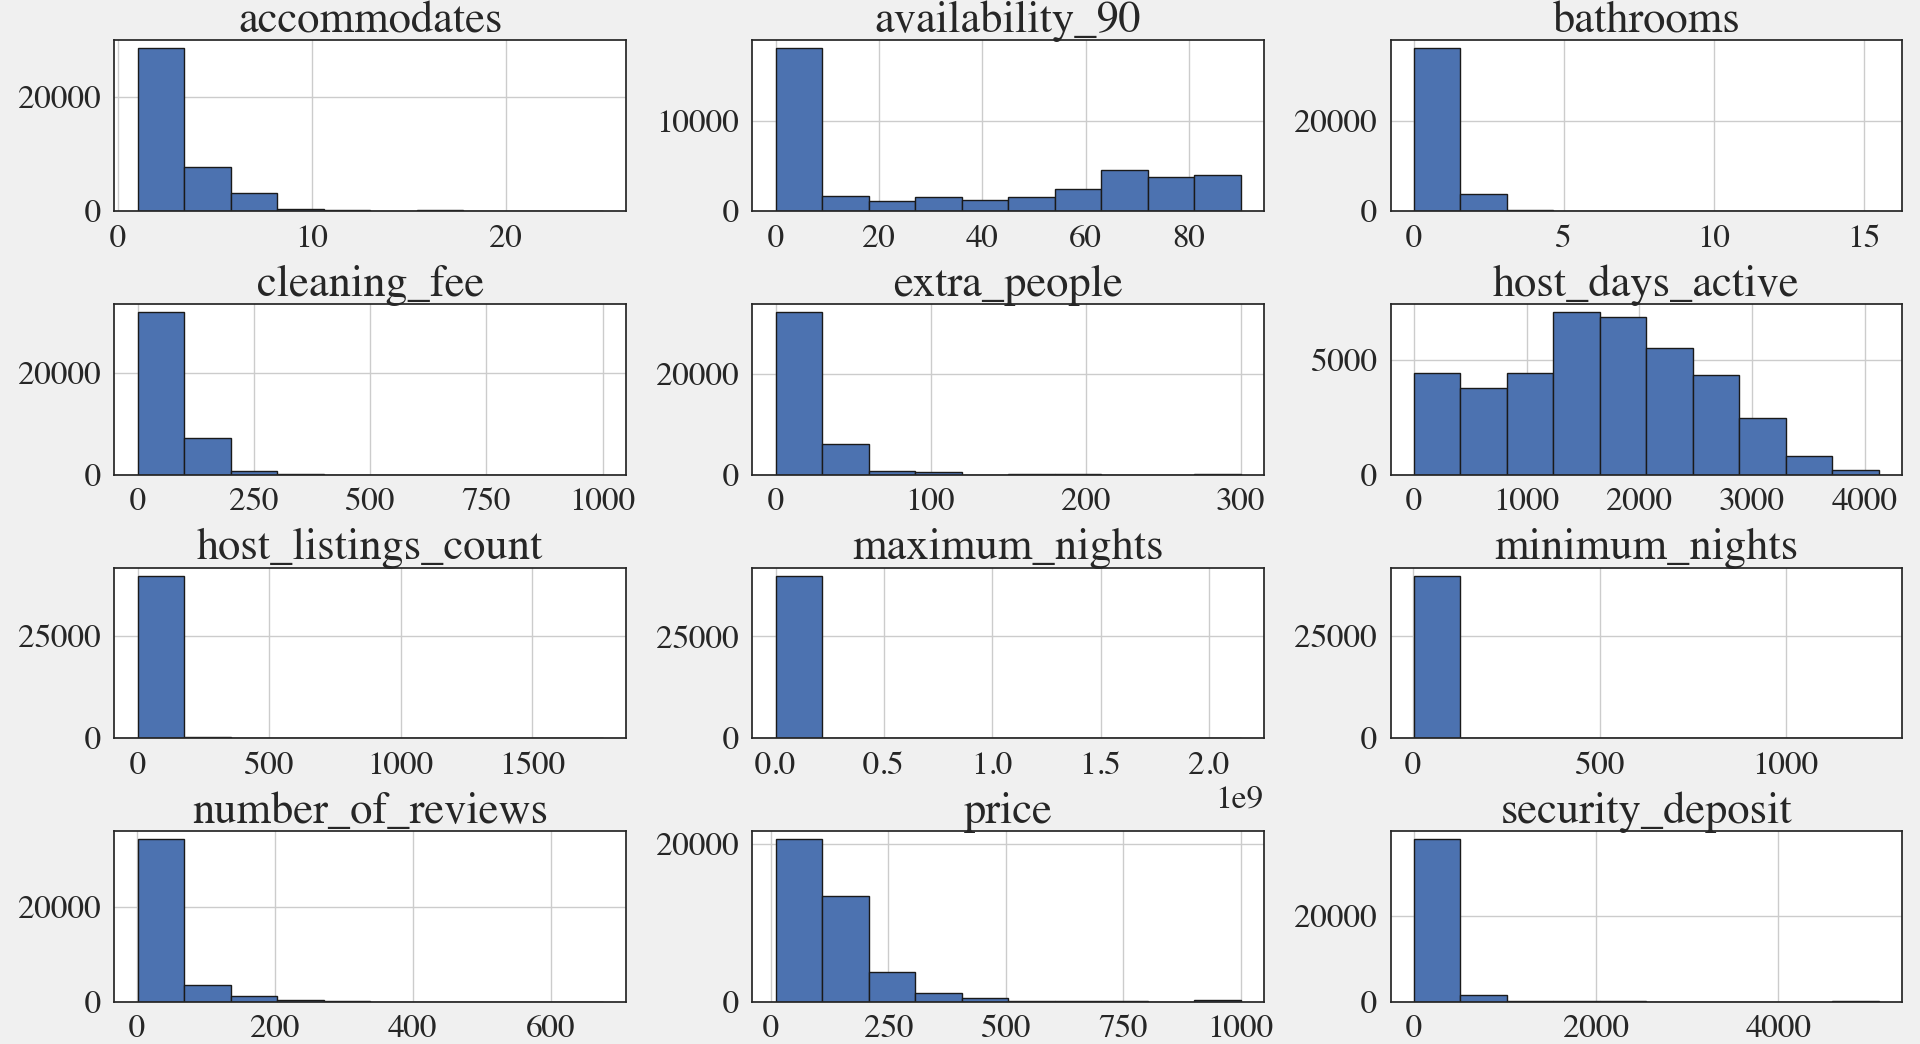
\includegraphics[width=\textwidth]{before-log.png}
\label{fig:histogram-before-transform}
\end{figure}

% from pre_processing.py
\begin{figure}[H] \centering
\caption{Histogram of Numerical Feature Distribution After Log Transform }
\includegraphics[width=\textwidth]{after-log.png}
\label{fig:histogram-after-transform}
\end{figure}



\clearpage
	\fancyhf{}
	\rhead{\thepage}
	\lhead{\textbf{ \nouppercase{\leftmark}} }
\phantomsection
\addcontentsline{toc}{chapter}{Bibliography}
\printbibliography

\end{onehalfspace}
\end{document}
